\documentclass{kththesis}
\usepackage{csquotes} % Recommended by biblatex
\usepackage[style=numeric,sorting=none,backend=biber]{biblatex}
\usepackage{amssymb}
\usepackage{hyperref}
\usepackage{amsthm}
\usepackage{amsmath}
\usepackage{mathtools}
\usepackage{listings}
\usepackage{minted}
\usepackage{tcolorbox}
\usepackage{color}
\usepackage{mips}
\usepackage{etoolbox}
\usepackage[framemethod=TikZ]{mdframed}
\usepackage{stackengine}
\usepackage{array}
\usepackage{makecell}
\usepackage{pxfonts}

%\DeclareFieldFormat{urldate}{
%    (Accessed \thefield{urlyear}-\thefield{urlmonth}-\thefield{urlday}\isdot)}

\newtheorem*{definition}{Definition}
\newcolumntype{?}{!{\vrule width 1pt}}

%Set up toc links
\hypersetup{
    linktoc=all,     %set to all if you want both sections and subsections linked
    linkcolor=black,  %choose some color if you want links to stand out
}

\addbibresource{references.bib} % The file containing our references, in BibTeX format

\title{Alternating Control Flow Graph Reconstruction by Combining Constant Propagation and Strided Intervals with Directed Symbolic Execution}
\alttitle{Alternaterande kontrollflödesgrafsrekonstruktion genom att kombinera propagerande av konstanter och klivande intervaller med riktad symbolisk exekvering }
\author{Thomas Peterson}
\email{thpeter@kth.se}
\supervisor{Roberto Guanciale} 
\examiner{Mads Dam}
\programme{Master in Computer Science}
\school{School of Electrical Engineering and Computer Science}
\date{\today}

%-----Custom Commands-----
\newcommand{\MONTH}{%
  \ifcase\the\month
  \or January % 1
  \or February % 2
  \or March % 3
  \or April % 4
  \or May % 5
  \or June % 6
  \or July % 7
  \or August % 8
  \or September % 9
  \or October % 10
  \or November % 11
  \or December % 12
  \fi}

%Used for the righsquigyarrow in the psuedo-codes   
%https://tex.stackexchange.com/questions/123219/writing-above-and-below-a-symbol-simultaneously
\newcommand\stackrqarrow[1]{%
    \mathrel{\stackon[2pt]{$\rightsquigarrow$}{$\scriptscriptstyle#1$}}}

%Feedback 
\newcommand{\fbcomment}[1]{{#1}}  
%Uncomment next line to remove comments
\renewcommand{\fbcomment}[1]{}  

\renewcommand{\it}[1]{\textit{#1}}

\renewcommand\fcolorbox[4][]{\textcolor{cyan}{\strut#4}} %Remove minted error boxes

\lstdefinestyle{frame}{
        columns=fullflexible,
        frame=single,
        mathescape=true,
        tabsize=4,
}

\lstdefinestyle{abstractInt}{
        aboveskip=1.4em,
        basicstyle=\linespread{2}\ttfamily\small,
        belowskip=0em,
        columns=fullflexible,
        frame=single,
        mathescape=true,
        tabsize=4,
}

\lstdefinestyle{algorithmOLD}{
    basicstyle=\linespread{1.2}\small,
    columns=fullflexible,
    emph={Input,Output,if,else,foreach,for,while,return},
    emphstyle=\textbf,
    frame=single,
    mathescape=true,
    numbers=left,
    tabsize=4,
    framexleftmargin=2em, %To have line numbers inside frame
    xleftmargin=2em, %Move the frame to the right
}

\lstdefinestyle{algorithm}{
    basicstyle=\linespread{1.1}\small,
    columns=fullflexible,
    emph={Input,Output,if,else,foreach,for,while,return},
    emphstyle=\textbf,
    mathescape=true,
    numbers=left,
    tabsize=4,
    framexleftmargin=2em, %To have line numbers inside frame
    xleftmargin=2em, %Move the frame to the right
}

\lstdefinestyle{top}{
  abovecaptionskip=-1pt
  float=tp,
  floatplacement=tbp,
}

\mdfdefinestyle{algorithmFrame}{
    outerlinewidth=0.25pt,
    outerlinecolor=black,
    innerleftmargin=2pt,
    innerrightmargin=2pt,
    innertopmargin=-5pt,
    innerbottommargin=-5pt,
    skipbelow=-5pt,%Decrease the space between the frame and the figure caption
}
%   Studies
\newmdenv[style=algorithmFrame]{algorithmFrame}

% Uncomment the next line to include cover generated at https://intra.kth.se/kth-cover?l=en
% \kthcover{kth-cover.pdf}


%---Notes---
%A conscientiously written scientific report in Swedish or English where the problem is introduced, different methods for the solution are discussed, the method chosen is presented, the solution and the results are described and the results are analyzed

%---Before Handing in the Report--
%Check if roman numbering should include list of tables/figures
%Ensure that figure footnote of figure 3.2 (CPA+ of jakstab) is on right page..

%Content checklist: https://www.kth.se/social/group/examensarbete-vid-cs/page/degree-project-checklist/

%Formalitiees checklist: https://www.kth.se/social/group/examensarbete-vid-cs/page/formalities-checklist/

%Read the opposition documents: https://www.kth.se/social/group/examensarbete-vid-cs/page/public-discussion-and-examination/

%Check that all sources look good! And try to double check correctness!
%---------------------------------
%---TODO---
%Ensure abbreviations(like CFG) are introduced with the first occurrence of the notion
%Ensure consistent usage of intel or AT&T x86 syntax
%Different fonts for headers and content?(See toc)
%Avoid using "we"
%Ensure all github links are correct
%---------------------------------

\begin{document}

% Frontmatter includes the titlepage, abstracts and table-of-contents
\frontmatter

\titlepage

\begin{abstract}
In this thesis we address the problem of control flow reconstruction in the presence of indirect jumps. We introduce an alternating approach which combines both over and under-approximation to increase the precision of the reconstructed control flow automaton compared to pure over-approximation. More specifically, the abstract interpretation based tool, Jakstab, from earlier work by Kinder, is used for the over-approximation. Furthermore, directed symbolic execution is used for under-approximating successors of instructions when these can not be over-approximated precisely. The results of our experiments show that strided interval analysis suffers in performance when encountering particularly challenging loops in the control flow automaton. Additionally, they suggest that our approach consumes a large amount of memory since it needs to extract and store a large number of possible paths to the unresolved locations. 
%\\ \\
%\textbf{Keywords}\\
%Binary analysis, Control flow reconstruction, concolic execution
\end{abstract}


\begin{otherlanguage}{swedish}
  \begin{abstract}
  I detta examensarbete studeras hur rekonstruction av kontrollflöde kan utföras i närvaro av indirekta jump instruktioner. I examensarbetet introduceras ett alternerande tillvägagångssätt som kombinerar både över och underapproximation för att öka precisionen av den rekonstruerade kontrollflödesautomaten jämfört med endast överapproximation. Mer specifikt används det abstrakta tolknings-baserade verktyget, Jakstab, från tidigare arbete av Kinder, för överapproximation. Vidare används riktad symbolisk exekvering för att under-approximera efterträdare till instruktioner när dessa inte kunnat överapproximeras med hög precision. Resultaten av våra experiment visar att analyser baserade på klivande intervaller tappar i prestanda när de möter en vis typ av loopar i kontrollflödesautomaten. Dessutom antyder resultaten att vårat tillvägangångssätt kan fordra en stor mängd minne då det kräver extraktion och tillfällig lagring av ett stort antal möjliga vandringar från programmets ingång till de olösta programpositioner.
  \end{abstract}
\end{otherlanguage}
%\clearpage
%\section*{Acknowledgement}
%I would like to thank my supervisor Roberto Guanciale, for his feedback and guiding throughout the research and writing of this report. 
%\\ \\
%Thank you! 
%\\ \\ \\ \\
%Stockholm, \MONTH \the\year
%\\ \\
%\it{Thomas Peterson}

\tableofcontents
\thispagestyle{empty}

\clearpage
\thispagestyle{empty}
\section*{Abbreviations}
%\textbf{AF:} Adjust Flag\\
\textbf{BBG:} Basic Block Graph\\
\textbf{BSS:} Basic Service Set\\
\textbf{COTS:} Commercial Off-The-Shelf\\
%\textbf{CF:} Carry Flag\\
\textbf{CFA:} Control Flow Automaton\\
\textbf{CFG:} Control Flow Graph\\
\textbf{CNF:} Conjunctive Normal Form\\
\textbf{CPA:} CPA Configurable Program Analysis \\
\textbf{DSE:} Directed Symbolic Execution\\
\textbf{IR:} Intermediate Representation\\
\textbf{IP:} Instruction Pointer\\
\textbf{Jakstab:} \textbf{Ja}va Tool\textbf{k}it for \textbf{Sta}tic Analysis of \textbf{B}inaries\\
%\textbf{OF:} Overflow Flag\\
%\textbf{PF:} Parity Flag\\
%\textbf{SF:} Sign Flag\\
\textbf{RAM:} Random Access Memory\\
\textbf{Stdout:} Standard Output\\
\textbf{SAT:} Boolean Satisfiability Problem\\
\textbf{SMT:} Satisfiability Modulo Theories\\
%\textbf{ZF:} Zero Flag\\

\clearpage
\thispagestyle{empty}
\section*{Glossary}
\textbf{CFG:} A BBG or a CFA.\\
\textbf{Conditional Jump:} A jump instruction which only performs a jump if a certain condition holds.\\
\textbf{Direct Jump:} A jump instruction which jumps to an explicit address.\\
\textbf{Double Word:} 4 bytes.\\
\textbf{Indirect Jump:} A jump instruction which jumps to an address located in a register or a memory location.\\
\textbf{Jump table:} A data structure which sometimes results from switch cases and leads to indirect jumps. \\
\textbf{Jakstab} A static analysis platform for x86 binaries. \\
\textbf{Unconditional Jump:} A jump instruction which performs a jump independently of the FLAGS register.\\
\textbf{Word:} 2 bytes.\\
%\textbf{Transpilation:} The act of translating a binary program into its equivalent IL program\\

\listoffigures
\thispagestyle{empty}
 
\listoftables
\thispagestyle{empty}

% Mainmatter is where the actual contents of the thesis goes
\mainmatter
\cleardoublepage
\pagenumbering{arabic}

%---INFO ABOUT CITATIONS---
%We use the \emph{biblatex} package to handle our references.  We therefore use the command \texttt{parencite} to get a reference in parenthesis, like this \parencite{heisenberg2015}.  It is also possible to include the author as part of the sentence using \texttt{textcite}, like talking about the work of \textcite{einstein2016}.

\chapter{Introduction}
%X The question is easy to identify, the project's purpose and objective are clear.
%X The problem (and the student's contribution) has defined limits, its relevance is justified and put in context
%
%Explain why we want to study the binary instead of the source code. Use example in WYSINWYX where memset was removed by compiler?
\fbcomment{\color{red}Goal: Introduce the reader to why the topic is relevant, what the problem statement is and the outline of the thesis}
Software is normally not developed directly in machine code but indirectly in a higher-level programming language such as C. Before a program can be used, its code must be compiled into architecture-dependent machine code. However, the compilation process can vary depending on many factors such as, for example, the type of compiler and the optimization level. Thus, software written in a non-assembly language might have multiple binary representations, some of which might even be erroneous\cite{preciseCFG}. As such, when analysing software, it might be incorrect to expect properties which hold in the source code to hold in the compiled binary. A prime example of this is the malicious copies of installers for the Xcode\cite{XcodeBook} framework that began circulating in 2015\cite{XcodeGhost}.
\\ \\ 
These installers appeared to behave identically to the legitimate installers but would install a corrupted version of the framework. Subsequently, during compile time, the corrupted framework would inject malware into the application. Thus, development with the infected framework would result in infected applications. Consequently, source-code level analysis would not have been able to find anything wrong with the produced applications. As such, this example clearly motivates why binary-level analysis is paramount. In addition to corrupted compilation processes, another incentive to binary-level analysis is that source code often is unavailable as many commercial off-the-shelf (COTS) software and third-party libraries are distributed only in binary form\cite{preciseCFG}.
\\ \\
As binary code is more verbose than high-level code, it is infeasible to manually analyze large binaries. Consequently, many binary analysis platforms have been created to automate binary analyses\cite{BitBlaze}\cite{BAP}\cite{TrABin}\cite{CodeSurfer}. Binary analysis has thus become a broad field with many different applications. It might, for example, be used for program verification\cite{TrABin}, exploit generation\cite{angr} or detection of memory management errors\cite{valgrind}. Further, binary analysis can be useful even in situations where the source code is available. Such situations can, for example, occur when the compiler is not part of the trusted computing base and one would like to empirically establish that properties of the source code still holds in the corresponding binary.
\section{Problem Statement}
%Falsify: DSE can not alternatingly be used to increase precision of abstract interpretation approahes.
%Problem statement: To what extent can DSE be used to increase precision of abstract interpretation based approaches?
%https://en.wikipedia.org/wiki/Reachability_problem
One fundamental obstacle when performing binary analysis is the lack of precise control flow information. There are already many existing approaches to control flow reconstruction. These can be categorized as static or dynamic techniques. Static techniques study a binary without performing concrete executions. Instead, they reason about the binary in an abstract manner. Dynamic techniques, on the other hand, concretely execute the binary with different inputs with the intention of triggering different control flow paths. 
\\ \\ 
Static analysis often suffers from problems stemming from indirect jump instructions. These are jump instructions where the processor is instructed to jump to a value stored in a register or memory location rather than an explicit address encoded in the instruction. As it is expensive to keep track of all memory and register content for all possible states of a program, it is expensive to calculate the target location of such jumps. Consequently, many static analysis tools resort to approximations which might not always result in an optimal control flow reconstruction.
\\ \\
The main objective of this thesis is to study how the precision of control flow reconstruction can be improved in the context of alternating over/under-approximation approaches. More specifically, it is studied how indirect jump resolution can be improved by using under-approximation when over-approximation can not deduce a finite set of possible successors to an instruction. The thesis is limited to 32-bit x86 binaries and targets binaries without additional source code information.
\\ \\
In this thesis, an approach based on alternating over/under-approximation inspired from previous work\cite{alternating} is investigated. Furthermore, the constant propagation and strided intervals used for over-approximation are based on previous work by Kinder et al\cite{Jakstab}. Finally, the under-approximation is performed through the usage of directed symbolic execution and an SMT solver. 
%"The automatic test generation will be conducted through white-box fuzzing and the over-approximation will use constant propagation as it scales well to large binaries\cite{Jakstab}. The goal will be to study to what extent precision and coverage can be improved if one were to use white-box fuzzing techniques instead of random fuzzing techniques in the context of over/under-approximation approaches. The algorithm will resort to under-approximation only when the over-approximation can not determine a finite amount of possible jump targets. In the case where both the under and over-approximation can not determine the targets, the branch will be assumed to be non-feasible. This has the benefit of avoiding to create a degenerate CFG by adding an edge from the branch location to every possibile location in the program."

\section{Outline}
\fbcomment{\color{red}Goal: Introduce the outline of the report (Will probably be a bit more specific in the final version of the report)}
The outline of the thesis is as follows. In chapter \ref{chap:background}, a theoretical background is provided. This background serves as a foundation for understanding the remaining parts of the thesis. In chapter \ref{chap:methodlogy}, the degree project methodology is presented and in chapter \ref{chap:results} the results are illustrated and described. Thereafter, in chapter \ref{chap:discussionAndConclusions}, a summary of the thesis and discussions concerning possible future work, are provided.
 
\chapter{Theoretical Background}\label{chap:background}
%X The student displays knowledge of theoretical background and previous related work (significant literature is mentioned and relevant material is used).
%X The background is coherent and relevant.
\fbcomment{\color{red}Goal: Provide enough background information to understand the concepts of the thesis and give the thesis context.}
This chapter provides a theoretical background explaining the theory needed to understand the remaining parts of the thesis. The chapter starts with a brief introduction to control flow in the x86 architecture followed by an explanation of different types of control flow graphs. Therafter, the advantages and disadvantages of static and dynamic analysis techniques are presented. 
\\ \\
Afterwards, abstract interpretation is introduced and the fundamentals of dataflow analysis are explained. Then, the theory behind the over-approximation tool Jakstab and the abstract domains that are used in this tool are described. Finally, we discuss related work and how they differ from what has been conducted in this thesis.
\\ \\
Throughout the thesis, a set of hand-made example binaries will be presented to illustrate the pros and cons of different approaches to control flow reconstruction. These binaries will be referred to as synthetic binaries. Furthermore, these binaries will be used for the synthetic evaluation of our approach presented in setion \ref{sec:synEval}.

%http://ee.usc.edu/~redekopp/cs356/slides/CS356Unit5_x86_Control.pdf
%Good reference: https://software.intel.com/sites/default/files/managed/39/c5/325462-sdm-vol-1-2abcd-3abcd.pdf 
\clearpage
\section{Control Flow in the x86 Architecture}\label{sec:controlFlowInX86}
\fbcomment{\color{red}Goal: Give the reader an understanding of what assembly instructions affect control flow and how}
Assembly instructions can be categorized into three possible control flow transitions\cite{CFGFromPowerPC}. The first type is fall-through instructions. These instructions are instructions which, after being executed, simply increments the Instruction Pointer (IP) with the size of the instruction. Consequently, the execution continues with the instruction immediately after the fall-through instruction. Instructions which do not classify as fall-through instructions are denoted as jump instructions. 
\\ \\
The last two types are direct and indirect jumps. Jumps are instructions which transfers the flow of execution by changing the IP register by a specified value. The difference between a direct and and indirect jump is that a direct jump is a jump to an explicit address whereas an indirect jump is a jump to an address stored in a register or a location in RAM. 
\\ \\
Furthermore, jumps can also be categorized into conditional and unconditional jumps. Conditional jumps are jump instructions that only perform a jump to a specified location if a certain condition holds. Otherwise, the IP is simply incremented by the instruction size to instruct the CPU to execute the next instruction. Conversely, unconditional jumps are jump instructions that always results in a jump to a specified location
\\ \\
The table below provides example instructions in x86, illustrating the difference between conditional and unconditional jump instructions as as well as direct and indirect jump instructions. Generally, x86 instructions are represented using either Intel or AT\&T syntax. In this thesis, x86 examples will be written using the Intel syntax.
\begin{table}[ht]
\centering
\begin{tabular}{lllll}
\cline{1-3}
\multicolumn{1}{|l|}{\textbf{}}              & \multicolumn{1}{l|}{\textbf{Direct}} & \multicolumn{1}{l|}{\textbf{Indirect}} &  &  \\ \cline{1-3}
\multicolumn{1}{|l|}{\textbf{Unconditional}} & \multicolumn{1}{l|}{jmp 0x00401078}    & \multicolumn{1}{l|}{jmp eax}           &  &  \\ \cline{1-3}
\multicolumn{1}{|l|}{\textbf{Conditional}}   & \multicolumn{1}{l|}{je 0x00401078}     & \multicolumn{1}{l|}{je eax}            &  &  \\ \cline{1-3}
                                             &                                      &                                        &  &
\end{tabular}
%\caption[A table illustrating the difference between unconditional and conditional jump instructions as well as direct and indirect jump instructions.]{A table illustrating the difference between unconditional and conditional jump instructions as well as direct and indirect jump instructions.}
\label{tab:jumps}
\end{table}
\noindent
\\
The instruction \textit{jmp 0x00401078} is an example of an direct and unconditional jump instruction. It is unconditional since it uses the \textit{jmp} instruction which instructs the CPU to jump to the specified address unconditionally. Furthermore, it is direct since the address \textit{0x00401078} is specified explicitly. Note that the address \textit{0x00401078} is arbitrary chosen for the sake of illustration and does not have any special meaning.
\\ \\
The \textit{jmp eax} instruction is an example of an indirect and unconditional jump instruction. It is indirect since the jump is performed to the address located in the register \textit{eax}. The \textit{je 0x00401078} and \textit{je 0x00401078} instructions are examples of conditional jump instructions. These are instructions that execute a jump only if a specific condition is satisfied, in this case, if and only if the last pair of previously compared registers were equal. 
\\ \\
%SF - 1 if MSB (aka sign bit) of result = 1 OK
%PF - 1 if Parity of Least significant byte is even OK
%CF - 1 if unsigned op2 > unsigned op1 (Only when sub borrows bit since cmp performs subtraction) OK
%OF - 1 if sign bit of OP1 != sign bit of result and sign(OP1) != sign(OP2) OK
%AF - 1 if Carry in the low nibble of result OK
Before a conditional jump is executed, the CPU normally executes an instruction to compare different register values. In x86, it is common to use the \textit{cmp} instruction which takes two arguments. It subtracts the second argument from the first and sets a set of register flags according to the result of the subtraction. %More specifically, the \textit{cmp} instruction modifies the \textit{SF}, \textit{ZF}, \textit{PF}, \textit{CF}, \textit{OF} and \textit{AF} flags. 
%The \textit{SF} flag is set if the difference is negative and the \textit{ZF} flag is set if the difference is exactly 0.
\\ \\
%Furthermore, the \textit{PF} flag is set if the difference has an even number of set bits in the least significant byte and the \textit{CF} flag is set if the second argument would be greater than the first in an unsigned comparison. Further, the \textit{OF} flag is set if the sign bit of the first argument is different from the sign bit of the second argument and the sign bit of the result. Finally, the \textit{AF} flag is set if the four least significant bits of the results did not result in a carry. When executing one of the \textit{je} instruction in the above examples, the CPU would check that the \textit{ZF} flag is set before performing a jump to the specified location since the \textit{je} instruction only jumps on equality.
%\\ \\
Apart from explicit jump instructions, there are also \textit{call} instructions which can alter the control flow of a program. Normally, \textit{call} instructions are used to invoke a procedure. Initially, the program pushes it's arguments to the stack (Or alternatively puts them in registers). Thereafter, the program executes the call instruction, which is a push of a return address to the stack and an unconditional jump to the start of the procedure. At the end of the proceddure, there is usually a return instruction \textit{ret}. The \textit{ret} instruction pops the stack to obtain the return address that was pushed by the call instruction. Then, it instructs the CPU to perform and unconditional jump to the obtained return address. 
\\ \\ 
In this work, the theoretical framework of the over-approximation treats a \textit{call} instruction as an unconditional \textit{jmp} instruction which pushes the address of the subsequent instruction to the stack. Furthermore, a \textit{ret} instruction is treated as unconditional indirect jump whose target is the topmost value of the stack.

%Control flow graph have one entry node but might have multiple exit nodes. Can also have multiple input nodes if one only looks at part of the program. For example, if one would like to reconstruct the CFG of a function, this function might be called from multiple positions in the program.
%"They explain that indirect jumps have five major sources: switch-statements implemented with a table lookup and indirect jump, exception handling, goto statements to pointer assigned labels and use of procedure pointers and dynamic method invocation in object oriented languages." lit stud
%Background of cfg, why use them
%\\ \\
%Chicken and egg problem between Data flow analysis and control flow graph reconstruction.
%\\ \\
%
%intra-procedural
%inter-procedural
%\\ \\

%See page 119 in jakstab thesis for pros and cons with cfa vs bbg
\section{Control Flow Graphs}
\fbcomment{\color{red}Goal: Introduce the concept of CFG, BBG and CFA as well as describing the diference between them. Additionally, explain when a generalised CFA isn't equivalent to the common CFA.}
The control flow of a program is defined as what instructions are executed in what order. A Control Flow Graph (CFG) is a directed graph which illustrates the control flow of a program. This graph is usually represented by either a Basic Block Graph (BBG) or a Control Flow Automaton (CFA). Consequently, when it is not important whether the graph is represented by a BBG or a CFA, the notion CFG will be used. 
\\ \\
A Basic Block Graph(BBG) is defined as a directed graph G = (V,E) where V is a set of nodes representing blocks of instructions, called basic blocks, and E is a set of edges representing all the possible transitions between the basic blocks. Each basic block consists of a set of fall-through instructions and at most one jump instruction at the end the block. 
\\ \\
As all fall-through instruction are contained in basic blocks, each edge in the CFG normally corresponds to either a direct or an indirect jump. However, there is an exception when there is a jump whose targets lies inside a basic block. For this exception case, the targeted basic block has to be split in two, resulting in an edge between the fall-through instruction located immediately before the targeted instruction of the jump and the location of the targeted instruction. 
\\ \\ 
A Control Flow Automaton(CFA), as originally defined by Henzinger et al\cite{lazyAbstraction}, is a graph where nodes represent states and edges correspond to statements representing control flow transitions between states. In our context, the CFA definition by Kinder\cite{Jakstab} is used. More formally, let $Stmt$ denote the set of abstract statements and $L$ the set of potential values of the IP. Then, a CFA for an intermediate language is defined as a tuple $<T,V,start,E>$, where $T \subseteq L$ is a set of program locations, $V$ is the set of registers\footnote{In essence, $V$ is the set of free names. It should be noted that this set is architecture specific and thus does not vary between x86 binaries. The set is part of the definition since the free names are used in the set of abstract statements.}, $start$ is an initial location such that $start \in T$ and $E$ is an edge relation $E \subseteq T \times Stmt \times T$. 
\clearpage
\noindent
When a CFA is depicted as a graph, the nodes represent program locations and edges correspond to statements in the relation $E$. In other words, a CFA is essentially a BBG where instructions labels the edges rather than the nodes. Consequently, CFA:s have the same level of expressiveness as BBG:s. However, unlike BBG:s, CFA:s can be generalized to have more expressiveness. More specifically, a generalized CFA is a CFA where nodes are groups of states based on some criterion. 
\\ \\
The conventional CFA is thus a special case of the generalized CFA where the only condition imposed on the nodes is the value of the IP register. An advantage of generalized CFA:s over BBG:s and CFA:s is that their nodes can naturally correspond to program states and the edges to state transformations. Consequently, as conventional BBG:s and CFA:s can only represent connections between instructions, generalized CFA:s can more accurately represent the control flow of binaries.
\begin{figure}[!t]
    \centering
\begin{tcolorbox}
\begin{minted}[xleftmargin=5pt,linenos,fontsize=\footnotesize]{nasm}
SECTION .data
msg     db      'Hello World!', 0x0A

SECTION .text
start:
        mov edi,10      ; Set the edi register to 10
compare:
        cmp edi,0       ; Compare edi with 0
        je quit         ; Jump to quit if edi=0
print:
        dec edi         ; Decrement edi by 1
        mov edx, 13     ; Set edx to the length of msg
        mov ecx, msg    ; Set ecx to the address of msg
        mov ebx, 1      ; Set ebx to standard out
        mov eax, 4      ; Set eax to the opcode of write
        int 0x80        ; Perform the syscall
        jmp compare     ; Jump to compare
quit:
        mov ebx, 0      ; Set ebx to 0
        mov eax, 1      ; Set eax to the opcode of exit
        int 0x80        ; Perform the syscall
\end{minted}
\end{tcolorbox}
\caption[Assembly code of the example BBG and CFA graphs.]{Assembly code of the example BBG and CFA graphs.}
    \label{fig:assembly}
\end{figure}
\clearpage
\noindent
To better understand this, consider the assembly code in Figure \ref{fig:assembly}. The string "Hello World!" is stored in the data section of the binary and the text section contains the code for writing "Hello World!" to stdout ten times. The code contains the labels start, compare, print and quit as these can be used as jump targets for the jump instructions. Initially, the program sets the value of edi to 10 as this register is used to count how many times the string has been printed to stdout.
\\ \\
The program then compares $edi$ to 0 and jumps to \it{quit} if this holds. Otherwise, it decrements $edi$ by 1 and fills the registers with values for performing a system call to write the string 'Hello World!' to stdout. The register $edx$ is set to the length of the string, $ecx$ to the address of the string, $ebx$ to the file descriptor of stdout and $eax$ to the opcode of the write instruction. After performing the write, the execution performs a jump back to the compare instruction to check if $edi$ is still more than 0.
\begin{figure}[!t]
    \centering
    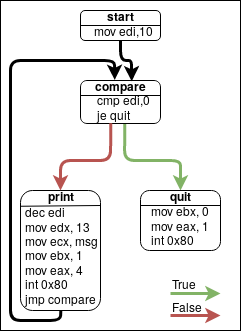
\includegraphics[scale=0.6]{Images/BBGExample.png}
    \caption[The BBG of the "Hello World!" Program.]{The BBG of the "Hello World!" Program. True and false branch conditions are illustrated with green and red arrows respectively.}
    \label{fig:HelloBBG}
\end{figure}
\noindent
\begin{figure}[!t]
    \centering
    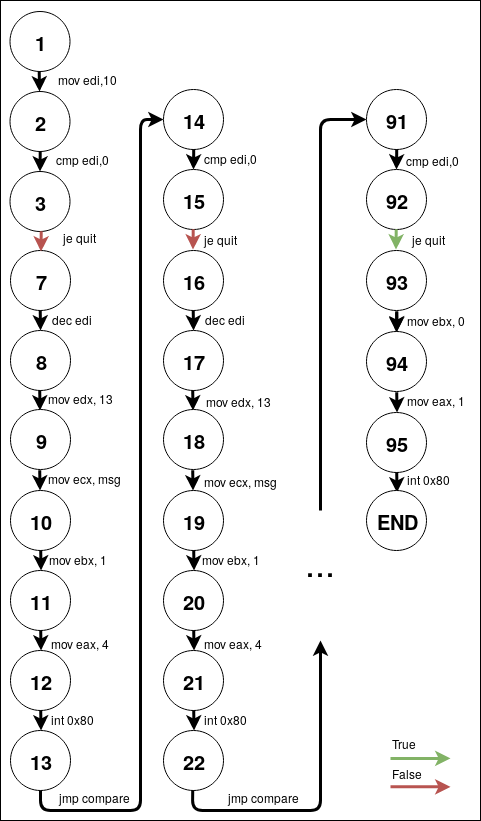
\includegraphics[scale=0.4]{Images/CFA.png}
    \caption[The generalized CFA of the "Hello World!" Program where nodes encompasses all register and memory information.]{The generalized CFA of the "Hello World!" Program where nodes encompasses all register and memory information. True and false branch conditions are illustrated with green and red arrows respectively.}
    \label{fig:HelloCFA}
\end{figure}
\clearpage
\noindent
The BBG of the hello-world program is illustrated in Figure \ref{fig:HelloBBG}. There are multiple problems with this BBG. Firstly, from the BBG, it appears that a possible path could be \it{start}, \it{compare} and \it{quit}. However, this path is not possible in practice. Furthermore, it is also not possible to tell if the program will ever terminate without studying the assembly code. This is because it appears that the program could execute \it{start} and then get stuck in an infinite loop between \it{compare} and \it{print}.
\\ \\
Assume that the criterion of the nodes of the generalized CFA is based on the complete register and memory content. Then, the generalized CFA of the hello-world program, depicted in Figure \ref{fig:HelloCFA}, only contains one possible path. This is because a node is no longer a group of instructions but rather a set of register values and a set representing memory content, thus accurately representing a concrete state. 
\\ \\
Consequently, state 2, 14 and 91 are distinct as they differ in the $edi$ value. More specifically, in this example, state 2, 14 and 91 correspond to $edi=10$, $edi=9$ and $edi=0$ respectively. Note, that the conditional jump instruction \it{je quit} does not have to correspond to two possible edges as the condition can be fully determined by the state.
%Add assumptions for figure 2.3(CFA of helloworld, i.e abs dom models all reg and mem content  note no socket, random numbers or file reads!)
%Add example depicting a bad abstraction that does not have deterministic state transitions. (?)
%CFA with loop terminates but CFA without loop we don't know if it terminates
\\ \\
A problem with the usage of BBG:s when representing control flow is when conducting control flow integrity enforcement\cite{CFIEnforcement}. When Control flow integrity enforcement is performed, the auditing software performing this enforcement uses information about what instructions can transfer control flow to which locations. It then audits executing programs to verify that all control flow transfers are performed according to these targets. If, however, a BBG is used, an attacker could enter a basic block from one edge and exit from an edge that shouldn't be feasible in practice when the entry edge was used. 
\\ \\
For example, if an attacker could manipulate the control flow of the hello world program so that it executed start, check and quit, this would be undetected by the control flow integrity enforcement. This problem is not solved by simply converting the BBG to a CFA representation of the control flow. Rather, one would need to generate and use a sufficiently accurate generalized CFA as this represenation would be able to distinguish between different concrete states at the same location.
%Mention example of control flow integrity(A CFG overapproximates double function calls, thus, using control flow hijacking it is possible to jump somewhere it shouldn't be possible)
% Soundess + accuracy example in graph + Cascading loss of precision
\begin{figure}[th]
    \centering
    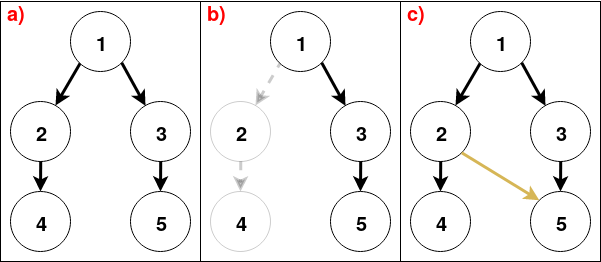
\includegraphics[scale=0.6]{Images/SoundAccurateGraph.png}
    \caption[An example of soundness and accuracy in CFG:s.]{An example of soundness and accuracy in CFG:s. Graph a is the ideal CFG, graph b is an accurate approximation of the ideal CFG and graph c is a sound approximation of the ideal CFG. The transparent nodes and arrows denote unidentified parts of the graph. Yellow arrows denote falsely identified edges.}
    \label{fig:SoundAccurateGraph}
\end{figure}
\\ \\
Two desirable properties of CFG:s are soundness and completeness, introduced by Shoshitaishvili et al\cite{angr}. Soundness is defined as the extent to which the CFG contains the correct control flow transitions. Thus a CFG is said to be sound if and only if, it contains all the possible control flow transitions. 
\\ \\
Similarly, completeness of a CFG is the extent to which the CFG only contains possible control flow transitions. Consequently, a CFG is said to be accurate if and only if, it only contains possible control flow transfers. In this work, completeness and the property of being complete will be referred to as accuracy and the property of being accurate respectively as we believe these terms are more intuitive.
\\ \\
In Figure \ref{fig:SoundAccurateGraph} the ideal CFG, an accurate under-approximation of the ideal CFG and a sound over-approximation of the CFG for some fictional binary program, is presented. Graph b is accurate since it contains all edges of the ideal graph. However, during reconstruction of graph b, the edge between node 1 and 2 was missed. Consequently, all nodes after node 2 were missed as well. One could imagine that there could be more instructions after node 2 that could only be reached through the edge between node 1 and 2. Thus, missing one edge during the control flow graph reconstruction can lead to a cascading loss of precision.
\\ \\
Graph c is a sound over-approximation of the ideal CFG. The problem with graph c is that the edge between node 2 and 5 has been added. This might, at first glance, not seem very problematic. However, it can, for example, be a security risk during control flow integrity enforcement. Furthermore, if there are a large amount of falsely identified nodes or edges the reconstruction time and memory usage can be significantly affected. In other words, over-approximation can consume significantly more time and memory resources than under-approximation since it has to explore more nodes and edges\cite{alternating}.
\\ \\
As there are currently no known polynomial time algorithms for creating the optimal CFG of an arbitrary binary, several researchers have resorted to under and/or over-approximation approaches\cite{preciseCFGBoolean}\cite{preciseCFG}\cite{CFGFromPowerPC}\cite{angr}. As purely over-approximating approaches, by definition, does not miss any edges of the ideal CFG, they are sound. Conversely, as under-approximation approaches never include superfluous edges, they are accurate. In this thesis, however, the primarily desire is to the maximize the precision.
\\ \\
The preciseness of a CFG can informally be thought of as the difference in the amount of edges and nodes of the subject CFG and the ideal CFG. Thus, an accurate CFG with 10 superflous edges is more precise than an accurate CFG with 20 superflous edges. A formal definition of preciseness of a CFG is provided in section \ref{sec:metrics}.
\\ \\
Unresolved control flow transitions primarily stems from the difficulty in resolving indirect jumps. Resolving indirect jumps requires data flow analysis which requires a CFG. However, CFG reconstruction requires resolving indirect jumps. Thus, there is a circular dependency. In the context of static analysis, this circular dependency is referred to as the "chicken and egg" problem\cite{Jakstab}.
%\\ \\
%In this work we do not distinguish between intra and inter-procedural branch instructions. Consequently, we do not use intra-procedural and inter-procedural CFG:s.

%-(Precise Control Flow Reconstruction Using Boolean Logic)-
%"Apart from switch-case statements, compilers generate indirect jumps/calls for function pointers or virtual methods."
%"Indirect control poses a so-called chicken-and-egg problem: In order to reconstruct the control flow graph from binary code, it is necessary to infer invariants that describe those registers which affect the target of an indirect jump/call."
%"the lack of a precise control flow graph often implies a drastic loss in terms of precision for any subsequent verification effort"
%
%Delay slots? 
%"Fortunately most compilers generate indirect jumps only in special cases" (Generic CFG)
%
%"Detecting the basic blocks of a binary program for a RISC-architecture is straightforward"(On the static analysis.. src 'Compilers, principles, techniques and tools')
%
%-(BitBlaze a New Approach...)-
%"Resolving indirect jumps usually requires program analyses that require a CFG"
%"Most normal analyses will first run an indirect jump resolution analysis in order to build a more precise CFG that resolves indirect jumps to a list of possible jump targets."
%VLIW makes things complicated because IP can jump in the middle of an instruction
%Explain why a very precise CFG reconstruction is important(Cascading loss of precision else-way).
%In this work we work with a CFA since these are better than CFG for expansions towards more analysis(since they are context sensitive and thus more expressive)
%CFA has distinct states for same instructions. This is similar to software model checking.

%Maybe mention that the generalized CFA can depict loop unrollment.

%Jakstab: "Call strings, however, are tied to the concept of procedures (which is unreliable in x86 assembly) and assume the existence of a separate call stack. This issue lead to the design of the path sensitive analysis presented in this dissertation."(Comparing jakstab with codesurfer)

\section{Static and Dynamic Analysis}
\fbcomment{\color{red}Goal: Explain challenges of static analysis. Also, pros and cons of using static and dynamic analysis}
%https://www.cs.cmu.edu/~aldrich/courses/654-sp08/slides/11-dataflow.pdf "static analysis can find mechanical errors" p7
%Binary Analysis platforms. Microsoft Boogie, Valgrind, LLVM and Mayhem.
%see "static Disassembly and Code Analysis"
%Techniques such as abstract interpretation, constraint solving, and type systems may be used for control-flow analysis.
The goal of static and dynamic analysis techniques are to determine properties and
functions of a program\cite{staticOfInd}. Static analysis is an umbrella term for all methods of program analysis which are conducted by examining a program without subjecting it to any concrete executions. Conversely, dynamic analysis comprises all of the program analysis techniques which are based on concrete executions of the studied program. %Furthermore, when the two types of techniques are mixed together, they are sometimes referred to as glass-box testing techniques\cite{DefinitionStaticAnal}.
\\ \\
Binary analysis platforms which leverage Static analysis techniques usually constitute of a hardware-independent representation, a mechanism to translate architecture dependent binaries to this representation as well as several architecture independent analyses that processes the hardware-independent representation\cite{TrABin}. Formally, the intermediate representation is normally represented using abstract interpretation\cite{Jakstab}. Abstract interpretation will be further described in section \ref{sec:AbsInt}.
%In this work, both static and dynamic analysis techniques are used to reconstruct a precise CFA from a given binary. Static analysis is used to over-approximate the CFA while dynamic analysis is used to under-approximate targets of unresolved jumps. The over-approximation is conducted using abstract domains which correspond to over-approximations of possible values for various registers and memory locations. 
%Furthermore, directed symbolic execution leveraged to symbolically execute specific sequences of instructions that end at unresolved locations. This results in a symbolic state which contains a symbolic expression for the next IP value. Then, an SMT solver is used to generate concrete IP values given the symbolic expression. A more detailed description of our approach is provided in chapter \ref{chap:methodlogy}.
\subsection{Disassembly in Static Analysis}
A core issue related to the analysis of programs is the problem of distinguishing code from data\cite{ABinaryRewriting}. As a consequence, static analysis techniques require some way to identify what bytes of a binary should be disassembled. These techniques are referred to as disassembly techniques. Disassembly techniques can, in general, be categorized as either being based on a linear sweep approach or a recursive traversal approach\cite{DisassemblyOfExecutable}. It should, however, be noted that none of these two approach are 100\% precise\cite{ABinaryRewriting}. Furthermore, there are also disassembly techniques which can not be categorized into these two categories such as speculative disassembly\cite{preciseCFG} or on-demand disassembly as performed in Jakstab\cite{Jakstab}.
\\ \\
Linear sweep approaches starts by disassembling the first byte at the start of the code section and then simply disassemble one byte after the other until an illegal instruction is encountered\cite{ABinaryRewriting}. This makes linear sweep based disassemblers easy to thwart as an attacker can simply place a jump in front of some malformed instructions. This would make the control flow follow the jump instruction to pass the malformed code but could stop linear sweep disassemblers as they would be unable to disassemble the malformed instructions\cite{ABinaryRewriting}. Some examples of linear disassembly tools are objdump, WinDbg and SoftICE\cite{ReversingSecretsofReverseEngineering}.
\\ \\ 
Recursive traversal approaches starts at the beginning of the code section as linear sweep approaches. However, instead of treating branch instructions as fall-through edges, recursive traversal approaches proceed by following each branch instruction encountered in a depth-first or breadth-first manner. Some examples of popular tools that use recursive disassembly are IDA Pro, OllyDbg and PEBrowse Professional\cite{ReversingSecretsofReverseEngineering}.
%See jakstab section 1.2
%Add jakstabs way of disassembling
%symbols + lack of types + no fixed procedure layout ? 
%For example, Giovanni Vigna introduced a disassembly technique which can deal with obfuscated binaries by using ..\cite{StaticDisAndCodeAnal}. 
%"Thus, robust techniques are required that can deliver reliable results even when exposed to binaries which do not follow conventions"
\subsection{Challenges of Static Analysis}
\fbcomment{\color{red}Goal: Describe what makes static analysis difficult(For example, instructions of varying sizes).}
Apart from the difficulties related to disassembly, static analysis also faces other challenges. One such challenge is the number of instructions in CISC architectures, such as x86, as these architectures normally have a very large amount of instructions and contains many specialized instructions for various specific tasks\cite{intelX86Manual}. For example, there are over 300 SIMD instructions in x86 for performing fast vector operators on multiple bytes or words at once\cite{vectorInstructions}. A static analysis which aims to over-approximate control flow can not simply ignore instructions but has to over-approximate all possible instructions on at least a coarse level. 
\\ \\
In addition to the large amount of instructions, some architectures, such as x86, allows for instruction of varying lengths. As such, instructions does not have to be aligned and overlapping instructions may thus exist. For example, if a 4 byte instruction exists at address x, a 3 byte instruction could possibly be hidden at address x+1. This is challenging for recursive and linear disassemblers but can be handled easier using on-demand disassembly as performed by Jakstab which we use for the over-approximations in this thesis. 
\\ \\
Static analysis can be further complicated when analyzing malware as malware can use techniques that obfuscate the binary representation of a program\cite{StaticDisAndCodeAnal}. As malware does not have to comply to calling conventions, they can abuse calls and returns to complicate attempts of reverse engineering. For example, a jump instruction such as \it{jmp eax} can be expressed as a push to the stack \it{push eax} followed by a return instruction \it{ret}. Additionally, malware sometimes leverages self-modification techniques where the instructions are modified on the fly. As such, all instructions do not exist in the binary file but are synthesised during execution, making this part of the execution troublesome to analyze.
\\ \\
Finally, a last challenge is analyzing instructions which use data stored in registers or memory whose content is unknown. These type of instructions are normally memory updates using pointer dereferences or indirect jump instructions which was described in section \ref{sec:controlFlowInX86}\cite{Jakstab}. Memory updates to unknown locations are particularly bad as they imply that an over-approximation has to assume that any location in memory might have been modified. As such, all known memory content has to be discarded if the approximation is to be kept sound.

\subsection{Dynamic Analysis}
%\fbcomment{\color{red}Goal: Describe pros and cons of dynamic analysis.}
\fbcomment{\color{red}Goal: Describe different alternatives to directed symbolic execution and why directed symbolic execution was selected(For example, the example of "if(x=2)")}
An approach to under-approximating the control flow of a binary is to use dynamic analysis. This can be performed by executing the binary with some carefully generated input and adding the execution trace to the CFA. To craft this input, it is possible to use fuzzing techniques.
\\ \\
Fuzzing techniques are in general categorized as black-box, gray-box or white-box techniques\cite{fuzzingSurvey}. Black-box techniques are techniques which treats the binary as a black box. Thus, black-box techniques only observes the input and output of the binary. Conversely, white-box techniques are techniques which exploit knowledge of the internals of the binary. Furthermore, Gray-box techniques are techniques which can not be categorized as purely white or black-box as they uses a mixture of the two techniques. As black box fuzzing typically exhibits low coverage, black-box techniques are typically not of interest in the context of CFG reconstruction\cite{fuzzingSurvey}.
\\ \\
A popular gray-box technique is mutation-based fuzzing. Mutation based fuzzers takes an initial seed which is an initial well-formed input. Thereafter, the seed is given to the binary and some information from the execution is obtained. This information is then used to create new seeds by mutating existing ones. Common mutation techniques are bit-flipping, arithmetic mutation, block-based mutation and semantic mutation\cite{fuzzingSurvey}.
\\ \\ 
White-box techniques are usually some sort of guided fuzzing, mutation or concolic execution\cite{fuzzingSurvey}. Guided fuzzing encompasses all techniques which leverage static or dynamic program analysis techniques for enhancing the effectiveness of the fuzzing process. Mutation includes techniques which modify the binary in a way that benefits the generated input seeds. For example, mutation can be used to remove a checksum check to ensure that all input pass the check\cite{fuzzingSurvey}.
\\ \\
During concolic execution, which is also known as dynamic symbolic execution, the program is initially executed with an initial concrete input. The input is then given to the binary in what is denoted as a concrete execution. During the concrete execution, symbolic expressions are recorded for the passed branches. Thereafter, an SMT solver can be given a variation of the obtained constraints to create a set of inputs that would take a specific path in the binary. This technique has the advantage of being more likely to generate inputs that improve coverage than random inputs\cite{fuzzingSurvey}. On the other hand, a disadvantage of using whitebox techniques, in general, is that they are often slower than gray or black-box techniques\cite{fuzzingSurvey}.
\\ \\
Constraint-based fuzzing techniques, such as concolic execution, focus on solving constraints to create inputs that take different paths in the binary. Consequently, this types of approaches could potentially be a more attractive technique than mutation based fuzzing when one wants to reconstruct the control flow of a binary as they make it is easier to analyze narrow input ranges.
\clearpage
\begin{figure}[!t]
    \centering
\begin{algorithmFrame}
\begin{lstlisting}[escapeinside={(*}{*)},style=algorithm]
void check(int x):
    if x == 25:
        printf("x is 25\n");
    else:
        printf("x is not 25\n");
\end{lstlisting}
\end{algorithmFrame}
\caption{An example where random black-box fuzzing will have a low probability of exploring all possible branches.}
    \label{fig:if25}
\end{figure}
\noindent
For example, consider the c code in Figure \ref{fig:if25}. This figure contains an if statement which is only taken if the value of the input x equals 25. Assume that x is supplied directly from standrad input as the first 4 bytes. Then, for random black-box testing, assuming 32-bit integers, there would be a probability of $\frac{1}{2^{32}}$ that $x$ would be $25$ and the first print statement would be executed. However, if white-box fuzzing was used, this probability could be increased dramatically by examining the internals of the program.
\\ \\
In this thesis, Directed Symbolic Execution is applied to obtain successors of indirect jumps who could not be determined using abstract interpretation. The difference between DSE and conventional symbolic execution is that DSE guides the symbolic execution along a set of paths. For example, in the example above, a path to the check function and if statement could be followed to recover a symbolic state at the if statement. Then, the symbolic constraints for the next value of the IP could be sent to an SMT solver which would return a set of solutions to the constrains corresponding to successor locations.

%-(Precise Control Flow Reconstruction Using Boolean Logic)-
%Traditional static techniques disassemble a program’s
%binary image statically and build the control flow graph (CFG) from
%the assembly-level representation of the program. They are limited
%in precision because of difficulty in statically resolving indirect
%branches. Dynamic techniques, on the other hand, suffer from poor
%coverage and scalability. Hybrid techniques based on combined
%dynamic and symbolic path exploration can improve code coverage,
%but still suffer from poor coverage and scalability because they rely
%on expensive constraint solving to generate alternative inputs to
%explore different control flow paths.

\section{Abstract Interpretation}\label{sec:AbsInt}
%See summary of https://www.youtube.com/watch?v=EF_6QaQ_M-s&t=20s
\fbcomment{\color{red}Goal: Give the reader a basic understanding of abstract interpretation.}
Abstract interpretation is a technique where concrete objects are represented as abstract objects. In general, there is a function, denoted by $\alpha$, converting a concrete element into its corresponding abstract representation. This function is usually referred to as the abstraction or representation function. Conversely, there is a function, denoted by $\gamma$, converting an abstract object into its corresponding concrete object. This function is referred to as the concretization function
\\ \\%Is this rice's theorem? 
The reason for not carrying out analysis directly using concrete semantics is that this results in a state explosion as analysing a program in all of its possible execution environments is an undecidable problem\parencite{FRPatrick}. Consequently, all non-trivial questions about the concrete semantics of a program are undecidable. However, if one uses abstraction to only analyze properties which are of interest to the analysis, it can be possible to analyze the selected properties in finite time.
\\ \\
To be able to understand abstract interpretation, we introduce partially ordered sets\parencite{EoMPoset} and Galois connections\cite{galoisConnections}. A partially ordered set(poset) consists of a set and a binary relation such that the binary relation, given two elements, indicate which of the elements should precede the other or that neither of them precedes the other. Additionally, the binary relation must be reflexive, anti-symmetric and transitive. The difference between partially and totally ordered sets is that the former allows elements in the set to be incomparable while the latter requires every pair of elements, belonging to the set, to be comparable.
\\ \\
A Galois connection is a binary relation between two partially ordered sets. There are two types of Galois connections: monotone and antitone. This thesis uses monotone Galois connections. Consequently, when a Galois connection is mentioned, it refers to a monotone Galois connection.
\begin{definition} \textbf{Galois connection}\\
Let $(A, \sqsupseteq_A)$ and $(B, \sqsupseteq_B)$ be two partially ordered sets. Furthermore, let $\gamma$ and $\alpha$ be monotone functions such that  $\gamma : A \rightarrow B$ and $\alpha : B \rightarrow A$. Then, ${(A, \sqsupseteq_A)}$, (B, $\sqsupseteq_B$), $\gamma$ and $\alpha$ form a Galois connection if for all $a \in A$ and $b \in B$:
\makebox[\linewidth]{$\gamma(a) \sqsupseteq_B b$ if and only if $a \sqsupseteq_A \alpha(b)$}
\end{definition}
\noindent
In abstract interpretation, a Galois connection is established between a concrete and an abstract domain. The concretization function $\gamma$ and the abstraction function $\alpha$ used to map elements in the abstract domain with elements in the concrete domain and vice versa. Furthermore, the two posets in the definition correspond to the abstract and concrete domain. In abstract interpretation, these posets are typically bounded lattices.
\clearpage
\noindent
%\\ \\%https://en.wikipedia.org/wiki/Lattice_(order)
A lattice is a poset where every pair of elements have a unique least upper bound and a unique greatest lower bound. The least upper bound is also known as the supremum or join. Similarly, the greatest lower bound is also known as the infimum or meet. Furthermore, if a poset only satisfies the requirement that each pair of elements have a unique least upper bound it is a join-semilattice.
\\ \\
Similarly, if a poset only satisfies the requirement that each pair of elements have a unique greatest lower bound it is a meet-semilattice. Thus, a lattice could also be defined as a poset which is both a join-semilattice and a meet-semilattice. A bounded lattice is a lattice which has a top element $\top$ and a bottom element $\bot$ such that, for each lattice element x, $\bot \leq x \leq \top$. Equivalently, a lattice is a bounded lattice if and only if every finite set of elements has a join and a meet. In this work, the posets of the abstract domains are join semi-lattices. 
\\ \\
In this thesis, we form a Galois connection between a concrete and abstract domain. Each element of the poset for the concrete domain corresponds to a set of concrete states, where a concrete state is an actual state of the CPU and its execution environment. More formally, each element of the poset for the concrete domain is an element of $\mathcal{P}(S)$ where $S$ is the set of all possible concrete states and $\mathcal{P}$ is the powerset of S. Furthermore, the binary relation for the concrete domain is set inclusion. 
\\ \\
Each element in the poset of the abstract domain is an abstraction of a set of concrete states. The binary relation of the abstract domain indicates if one abstract domain element is subsumed by another. The semantics of this binary relation is dependent on what abstract domain is used. In this work, the abstract domains that were used were based on constant propagation and strided intervals which will be explained in further details in section \ref{sec:absDom}.

% Mention transfer function maybe....... 
%widenings and narrowings
%Complete lattice?
%Ascending chain condition
%Abstract semantics are a superset of the concrete semantics (https://www.di.ens.fr/~cousot/AI/IntroAbsInt.html#Cousot81-1)
%We say that an abstraction is sound (or correct) if the abstract semantics covers all possible cases of the concrete semantics. All formal methods are required to use sound abstractions: if a potential error is not signaled that it should be definitely impossible. Contrary to testing/debugging formal methods provide full coverage.(https://www.di.ens.fr/~cousot/AI/IntroAbsInt.html#Cousot81-1)

%To be a partial order, a binary relation must be reflexive (each element is comparable to itself), antisymmetric (no two different elements precede each other), and transitive (the start of a chain of precedence relations must precede the end of the chain). 

%"Intervals are better than exact sets because with exact sets algorithms used can be guaranted to finish in finite time."(powerpc?) 
%Rice's theorem

%"If the number of assumptions about the code is to be minimized, it is necessary to use an abstract domain for the analysis that is able to precisely represent target addresses." (jakstab)

% The concrete semantics of a program is an "infinite" mathematical object which is not computable: it is not possible to write a program able to represent and to compute all possible executions of any program in all its possible execution environments. Hence, all non trivial questions about the concrete semantics of a program are undecidable: it is not possible to write a program able to answer any question about the possible executions of any program (since the concrete semantics of this program would have to be computable). https://www.di.ens.fr/~cousot/AI/IntroAbsInt.html

%The join and meet of a subset S are respectively the supremum (least upper bound) of S, denoted ⋁S, and infimum
%A partially ordered set that is both a join-semilattice and a meet-semilattice is a lattice.
%https://en.wikipedia.org/wiki/Join_and_meet

%\section{Under-Approximation Approaches}

%https://homepages.dcc.ufmg.br/~fernando/classes/dcc888/ementa/slides/WorkList.pdf Worklist algo
%https://www.cs.cmu.edu/afs/cs/academic/class/15745-s03/public/lectures/L4_handouts.pdf
\clearpage
\section{Dataflow Analysis}
\fbcomment{\color{red}Goal: Give the reader an understanding of the context of the CPA algorithm(The core worklist algorithm which which is based on theory from dataflow analysis)}
Dataflow analysis is the problem of, for each program location, assigning a lattice element which over-approximates the possible concrete states at that program location\cite{cpaAlgo}. Usually dataflow analysis uses the program's BBG to determine to which parts of the program, values of variables might propagate. The most precise over-approximation can be determined by finding the least fixpoint. This can be performed by applying the transfer relation to abstract states and join the result with previous result at the corresponding program location. To determine whether the fixpoint has been reached or not, it is common to use a worklist which stores dataflow facts\cite{cpaAlgo}.
\\ \\
Techniques for dataflow analysis can be categorized into two categories; forward flow and backward flow analysis. In forward flow analysis, each exit node of a basic block is expressed as a function of the entry node of the basic block. Conversely, in backward flow analysis, entry nodes are expressed as functions of exit nodes of the corresponding basic blocks. This function is referred to as the transfer function.
\\ \\
The semantics of the transfer function is defined by the semantics of the instructions inside the basic blocks. Forward analysis typically requires an initial entry state to be defined. This entry state is used as the starting point of the propagation of dataflow information and can, for example, contain the fact that no variables have any known values. Similarly, backward flow analysis requires an initial exit state to be specified. Examples of forward and backward flow analysis techniques are reaching definitions and liveness analysis respectively.
\\ \\
It is possible to conduct dataflow analysis techniques on a different granularity than basic blocks. For example, they can be applied on the instruction level by using a relation between the entry node and exit node of each instruction. This is normally referred to as local analysis\cite{carneigeDataFlow}. However, it is more common to work at the basic block level and then use local analysis inside basic blocks when instruction-level dataflow information is desired\cite{carneigeDataFlow}. In this thesis, we do not reconstruct a BBG. Rather, we aim to reconstruct a precise CFA. As such, the transfer function of our abstract domain is defined by semantics at the instruction level. 
%http://web.cs.iastate.edu/~weile/cs641/5.DataFlowAnalysis.pdf
\clearpage
\begin{figure}[t]
    \centering
\begin{algorithmFrame}
\begin{lstlisting}[escapeinside={(*}{*)},style=algorithm]
in[$B_s$] := $X_0$
for each basic block $B$
    out[$B$] := $\bot$
    
$worklist$ := {$B$: $\forall$ basic blocks $B$}
while($worklist \neq \emptyset$)
    $B$ := remove($worklist$)
    in[$B$] := $\sqcup$ {out[$B^{\prime}$]: $B^{\prime}$ $\in$ pred($B$)}
    
    if out[$B$] $\neq$  $F_B($in[$B$]$)$
        $worklist$ := $worklist$ $\cup$ succ($B$)
        out[$B$] := $F_B($in[$B$]$)$
\end{lstlisting}
\end{algorithmFrame}
\caption[Example of a forward flow analysis worklist algorithm.]{Example of a forward flow analysis worklist algorithm.}
    \label{fig:WorklistAlgo}
\end{figure}
\noindent
An example of a worklist algorithm for a forward flow analysis is provided in Figure \ref{fig:WorklistAlgo}. This algorithm assumes that a BBG is available to determine the predecessors pred($B$) and successors succ($B$) of a basic block $B$. Furthermore, the information of the entry and exit of a basic block $B$ is denoted by in[$B$] and out[$B$] respectively. Initially, the input information of the starting block $B_s$ is set to a specific pre-defined value $X_0$. For each basic block, the exit information is then set to the empty lattice element $\bot$, signifying that no information is known. The worklist is then initially filled with all basic blocks of the BBG and the while-loop is entered.
\\ \\
In the while loop, a random basic block $B$ is removed from the worklist. The entry information of this block is then recalculated depending on the information of its predecessors using the join operator. Given a set of lattice element, the join operator creates a lattice element which subsumes every lattice element in the given set. Thus, the resulting element is an over-approximation of the possible data flow facts at the basic block $B$. Then, the algorithm checks if the new output of $B$, obtained by applying the transfer function $F_B$ to the input information of $B$, is different from the previous output information of $B$. If this is the case, the output information of $B$ is updated with the new generated information and all successors of $B$ are re-added to the worklist as their input information is dependent on the output information of $B$.
\\ \\
Eventually, the join won't result in any new information for the in[$B$] of a basic block $B$. Consequently, the output of the basic block is unchanged and no blocks are added to the worklist. When this has happened to all basic blocks and the worklist is empty, a fixpoint has been reached. This means that for each basic block $B$, out[$B$] over-approximates the possible dataflow facts outputted from $B$.
\\ \\
As dataflow requires the BBG whose reconstruction is dependent of dataflow facts, it is not trivial how one would reconstruct one without the other. However, Kinder\cite{Jakstab} devised an algorithm that can perform CFA reconstruction and deductions of dataflow facts simultaneously. In this thesis, this algorithm is used for the over-approximation part of the alternating approach presented in chapter \ref{chap:methodlogy}.
%Dataflow analysis can for example be used for code optimization by avoiding redundant or superflous computations. Furthermore, it can also be used for code validation through invariant generation\cite{BordeauxSoftwareVerification}.


%Worklist algorithm: https://en.wikipedia.org/wiki/Reaching_definition
%\section{Application Binary Interface}
%An Application binary interface(ABI) defines the rules of communication between a binary and the underlying operating system.
%\section{ELF structure}

\section{Over-Approximation with Jakstab}
\fbcomment{\color{red}Goal: give the reader an overview of jakstab and enough understanding of the notation in the phd thesis of Jakstab(So that this can be used in later sections such for example as the section about CPA modifications). Also, introduce concepts such as tops and bottoms in the context of the Jakstab tool}
Jakstab\cite{Jakstab} is an abstract interpretation based static analysis framework which combines control flow and data flow analysis to solve the chicken and egg problem of control flow reconstruction. It uses on-demand disassembly and an intermediate language to over-approximate the CFA of a binary. Contrary to conventional disassemblers, the on-demand disassembly makes it possible for jakstab to disassemble overlapping instructions. 
\\ \\
To abstract the details of assembly language while still capturing its relevant branching behaviour, Jakstab uses and intermediate language(IL). The author of the platform defines a set of abstract statements denoted by \it{Stmt}. Assume that $e_1,e_2 \in Exp$ where $Exp$ is the set of possible expressions. Then, the set \it{Stmt} consists of b-bit memory assignments $m_b[e_1] := e_2$ to a location $e_1$, conditional indirect jumps $if\;e_1\;jmp\;e_2$ where the $IP$ is set to $e_2$ if $e_1$ evaluates to true, assume statements $assume\;e1$ and a halt statement $halt$. As the intermediate language is free from side-effects, each assembly instruction of the binary is mapped to one or more abstract statements. As such, each abstract statement can be identified by an address of a concrete location and an index. 
\clearpage
\noindent
The only data type of the IL are integers. Consequently, booleans are represented by $0$ and $1$ corresponding to false and true respectively. Furthermore, the finite set of program locations is denoted by $L \subseteq \mathbb{N}$. This set contains all addresses of the program. A program is denoted as $<\ell_0,P>$ where $\ell_0$ is the starting location and $P$ is a finite mapping from program locations to statements and successors, More formally, $P$ is defined as $P:: L \rightarrow (Stmt \times L)$. Furthermore, the statement stmt at location $\ell \in L$ with successor $\ell^{'}$ is denoted by $[stmt]^{\ell}_{\ell^{'}}$. 
\\ \\
The assume statements results from various types of jump instructions. For example, they can result from a \it{jeq} instruction which succeeds a \it{cmp} instruction comparing \it{eax} to the value $2$. This would create two possible transitions, one where \it{eax} is equal to $2$ and the jump is taken as well as one where \it{eax} is not equal to $2$ and the jump is not taken. If the location of the \it{jeq} is denoted by $\ell$, the location of the immediately following instruction by $\ell^{'}_{2}$ and the target of the jump by $\ell^{'}_{2}$, the two resulting statements can be written as $[assume\;eax \neq 2]^{\ell}_{\ell^{'}_{1}}$ and $[assume\;eax = 2]^{\ell}_{\ell^{'}_{2}}$.
\\ \\
In some cases, Jakstab might not be able to resolve one or more successors for a location $\ell \in L$. This can occur when the statement stmt is an indirect jump for which the target could not be over-approximated. When this happens, Jakstab warns the user that the analysis will be unsound and continues exploring the binary at other locations where the analysis has yet to reach a fixpoint. Additionally, the unresolved location $\ell$ is marked to have the successor $\top$, which signifies that the successor location $\ell^{'}$ can be any location in the program, in essence that $\ell^{'} \in L$. The $\top$ symbol is used as it subsumes any possible lattice element in the location domain, which will briefly be introduced in section \ref{sec:absDomLoc}. 
%Add cpa algorithm?
%\\ \\ 
%Note that there is nothing such as a top node in the ideal graph since a top node, by definition, is a node whose successors are unknown and the ideal graph does not contain any nodes with unkown successors.

%Assume statements stem from guarded jumps
%Definition jak 3.2?
%Abstract reachability tree

%Resolve operator(jak 3.4.1)
%Statment map
%Transformer factory
%The il language + Overview of how jakstab works (Disasembling instructions on the fly)

%Jakstab: Pesimisitc vs optimistic vs semi-optimistic. Increase coverage?
%Strong vs weak updates? 


\section{Abstract Domains}\label{sec:absDom}
%See jakstab 3.4
%Add definition of abstract domain i.e: (post,eval,U,...)
\fbcomment{\color{red}Goal: Describe the abstract domains of Jakstab and what pros and cons come with each of them.}
%Widening operator
In this section the abstract domains used for the over-approximation are briefly and informally introduced. All of the abstract domains have a corresponding formal definition in Kinder's dissertation\cite{Jakstab}. First, the location analysis domain is briefly described in section \ref{sec:absDomLoc}. Thereafter, the constant propagation domain is explained in section \ref{sec:absDomCon}. Finally, the strided interval analysis is detailed in section \ref{sec:absDomInt}. These sections will contain assembly examples to illustrate when they are useful. For these and other assembly code examples, each line of code will be paired with a comment to help readers unfamiliar with x86 assembly.

\subsection{Location Analysis}\label{sec:absDomLoc}

The location analysis domain allows to omit location information from other abstract domains\footnote{For more information, see previous work by Kinder\cite{Jakstab}.}. It contains a label of an intermediate level instruction, which is an address to a concrete instruction and an index as each concrete instruction can correspond to multiple intermediate level instructions. The location Analysis is never used on its own. Instead, it is always combined with another abstract domain.

\subsection{Constant Propagation}\label{sec:absDomCon}
\fbcomment{\color{red}Goal: Introduce constant propagation and show a basic example of how it is used.}
The constant propagation domain consists of constant propagation and constant folding. Constant propagation signifies that constants are propagated through instructions so that register operands can be substituted with concrete values. Furthermore, constant folding signifies that constant expressions are calculated and substituted by the result of their evaluation.
\\ \\
For example, consider the synthetic program \it{cjmp.asm} depicted in Figure \ref{fig:cjmp.asm}. The text section is the section containing the instructions of a binary. Its start is declared at line 1. Then, line 2 declares the \it{\_start} label to be global, making it possible for the linker to know where the binary should start. The binary starts at line 5 by moving the constant value 0 into the register \it{eax}. Thereafter, through line 6 to 10, a series of registers operations are performed. These operations results in the the values 0 and 22 to be stored in the \it{eax} and \it{edi} register respectively. The \it{cmp} instruction at line 11 is then executed to set the flags according to the comparison between eax and 0. Since eax is 0, the zero flag \it{ZF} is set to one. Consequently, the instruction on line 12, which performs a jump to \it{exit} if \it{ZF} flag is set\footnote{The \it{ZF} flag is set when the subtractions performed in the \it{cmp} instruction results in zero. In essence, the \it{ZF} flag is set if the two compared values are equal.}, jumps to \it{exit} and the program terminates. 

\begin{figure}[!ht]
    \centering
\begin{tcolorbox}
\begin{minted}[xleftmargin=5pt,linenos,fontsize=\footnotesize]{nasm}
SECTION .text
global _start

_start:
        mov eax, 0      ; eax = 0
        add eax, 20     ; eax = eax + 20
        mov edi, 12     ; edi = 12
        sub eax, 30     ; eax = eax - 30
        add edi, 10     ; edi = edi + 10
        add eax, 10     ; eax = eax + 10
        cmp eax, 0      ; Compare eax with 0
        je exit         ; if ZF=1 jump to <exit>
unreachable:            
        jmp unreachable ; Jump infinitely
exit:
        mov ebx, 0      ; Set exit code to 0
        mov eax, 1      ; Set eax to sys_exit
        int 0x80        ; Syscall
\end{minted}
\end{tcolorbox}
\caption{cjmp.asm - An example containing a conditional jump which can be resolved without false positives using the constant propagation domain.}
    \label{fig:cjmp.asm}
\end{figure}
\noindent
\\ \\
Evaluation using the constant propagation domain starts with an empty state. The first instruction is then parsed into an instruction \it{eax = 0} and the value of 0 is stored in the register eax. Then, the next instruction is parsed resulting in the instruction \it{eax = eax + 30}. At this point, the value \it{eax = 0} is propagated to this instruction, turning it into the instruction \it{eax = 0 + 20} which is simplified to \it{eax = 20} and stored in the new state. The next instruction, at line 7, is parsed and the state becomes \it{\{eax=20,edi=12\}}.
\\ \\
The next instruction \it{eax = eax - 30} is loaded, \it{eax} is substituted with 20 and constant folding is performed to obtain the state \it{\{eax=-10,edi=12\}}. Thereafter, the same procedure repeats for the last two instructions \it{edi = edi + 10} and \it{eax = eax + 20} resulting in the state \it{\{eax=0,edi=22\}}. Now, the constant value of \it{eax} can be propagated to the succeeding compare instruction substituting eax in the expression and resulting in the instruction \it{cmp 0,0}. Consequently, the \it{ZF} flag can be determined to be one and the jump instruction at line 12 can be determined to only have the successor at line 16, eliminating a false positive edge in the CFA to the unreachable jump instruction. 
\\ \\
While constant propagation has the benefit of being able to scale well to larger programs\cite{alternating}, it has the disadvantage of not being able to resolve successors of return instructions. The reason is that constant propagation does not assume any initial values for memory locations and registers, and thus does not know the initial value of the stack pointer which is in turn requried to capture the effect of the \it{call} instruction. Consequently, when the \it{ret} instruction is later executed, the address at the top of the stack is unknown. Another limitation of constant propagation is that it only allows each state to have one possible value per register and memory location. This limitation will be illustrated by the example in the next section where it will be shown when it can be more appropriate to use the strided interval domain rather than the constant propagation domain.

\subsection{Strided Intervals}\label{sec:absDomInt}
\fbcomment{\color{red}Goal: Introduce strided intervals and show an example of when it is more useful than constant propagation.}
The elements of the strided interval domain consist of tuples with three elements. These three elements are integers for a minimum, maximum and a stride value. More formally, a strided interval is defined as: 
\begin{definition}\textbf{Strided Interval}\\
A strided interval is an interval $s[l,u]=\{l + s * n\;|\;l \leq l + s * n \leq u, n \in \mathbb{N}_0 \}$ where $s,l,u \in \mathbb{N}_0$ and $\mathbb{N}_0$ is the set of natural numbers including the zero element.
\end{definition}
\noindent The stride of a strided interval can be thought of as the difference between two adjacent elements of the interval. For example, the interval $2[4,8]$ is equivalent to the set $\{4,6,8\}$ since it contains the lower bound 4 and values separated by a stride of 2 up to the upper bound 8. As a consequence, conventional intervals can be represented as strided intervals where the stride is equal to 1. Furthmore, a stride of 0 signifies a singleton set containing only the lower bound of the interval, for example, $0[2,2] = 2$.
\begin{figure}[ht]
    \centering
\begin{tcolorbox}
\begin{minted}[xleftmargin=5pt,linenos,fontsize=\footnotesize,mathescape=true]{nasm}
SECTION .bss
buf      resb 4                 ; Reserve 4 bytes of
                                ; memory
SECTION .text
global _start

increment:
        add ebx, 1              ; ebx = ebx + 1
        jmp continue            ; jump to <continue>
_start:
        mov  edx, 4             ; length of buffer
        mov  ecx, buf           ; pointer to buffer
        mov  ebx, 0             ; stdin
        mov  eax, 3             ; sys_read
        int  0x80               ; perform syscall

        mov eax, dword [buf]    ; eax = $\top$
        mov ebx,0               ; ebx = 0
        cmp eax,1               ; compare eax with 1
        je increment            ; if eax = 1 jump
                                ; to <increment>
continue:
        add ebx, exit           ; ebx = ebx + <exit>
        jmp ebx                 ; jump to ebx
exit:
        nop                     ; No operation (1 byte)
        mov ebx, 0              ; Set exit code to 0
        mov eax, 1              ; sys_exit
        int 0x80                ; Syscall
\end{minted}
\end{tcolorbox}
\caption{branch.asm - An example of when strided intervals can be more useful than constant propagation.}
    \label{fig:branch.asm}
\end{figure}
\clearpage
\noindent
Strided intervals are useful to represent states at program locations where a register or memory location can contain more than one value. This will be illustrated through an example. Consider the assembly code of \it{branch.asm} depicted in Figure \ref{fig:branch.asm}. In addition to the text section, we instruct the Basic Service Set(BSS) section to reserve four bytes for our program at line 2. 
\\ \\
When executed, the program begins at the \it{\_start} label and starts by setting up the registers to perform a system call using \it{sys\_read}. At line 15, the CPU is instructed to perform the system call to read four bytes from standard input into the buffer buf which is located in the BSS section. This is done by performing a context-switch where the CPU is put in kernel mode where it has additional privileges and can perform the read into the buffer. The CPU then performs the read followed by a transition into user mode and a context switch resuming the execution of the program at the instruction after the syscall instruction.
\\ \\ 
At line 17 the content of \it{buf}, which contains the first 32 bits of the user's input, are copied into the 32-bit register \it{eax}. Thereafter, the \it{ebx} register is initialized 0, as it will be used as a counter. Then, \it{eax} is compared with 1 to determine if control should be transferred to the \it{increment} label or directly to the \it{continue} label. In the first case, the CPU executes line 8 to increase \it{ebx} by 1 and then jumps to line 23. At line 23 the offset of the \it{exit} label is added to the \it{ebx} register. Afterwards, a jump to the content of \it{ebx} is performed. At this point, \it{ebx} is either equal to \it{exit} or \it{exit + 1}. Note, however, that the instruction located at \it{exit} is a \it{nop} instruction of size 1 byte. Consequently, the CPU will execute either the \it{nop} instruction and continue from line 27 or continue from line 27 directly. Thus, the semantics of the program are independent of the user input. 
\\ \\
At the start of execution the interval analysis starts with a state only containing a strided interval with a stride of 0 for the stack pointer. After executing the syscall, each of the four registers used to pass parameters to the syscall, are represented by intervals of a stride of 0. Then, the \it{mov} instruction at line 17 is executed to load the content of the buffer into the \it{eax} register. However, as it is impossible to determine what user input is entered without actually executing the program, it is not possible to know what \it{buf} will contain after the syscall and thus not what will be loaded into the \it{eax} register at line 17. Consequently, the strided interval for \it{eax} will be removed from the state, i.e \it{\{eax=0[3,3], ebx=0[0,0], ecx=0[buf,buf], edx=0[4,4]\}} becomes \it{\{ebx=0[0,0], ecx=0[buf,buf], edx=0[4,4]\}}.
\\ \\
After loading the content of buf into \it{eax}, the \it{ebx} register is set to 0 and then the eax register is compared with 1. However, as there is currently no knowledge of eax in the state, it has to be assumed that all different flag values are possible after this statement. Consequently, when the \it{je increment} statement is reached, it has to be assumed that execution can continue on either line 8 or 23. Consequently, the state is split into one state where \it{ZF=1} and the execution continues at line 8 as well as one where \it{ZF=0} and the execution continues at line 23. 
\\ \\
The analysis which continued on line 8 will increase the value of \it{ebx} by 1 by changing the strided interval \it{0[0,0]} to \it{0[1,1]}. Then, the jump instruction is taken to line 23. Now there are two states which can be merged at this location, resulting in a state containing a wider strided interval \it{ebx=1[0,1]]}. The \it{exit} label is then added to the interval of \it{ebx} and the indirect jump to the content of \it{ebx} is performed. Since, a strided interval can model the two possible values of ebx, it can be determined that \it{jmp ebx} results in a jump to either \it{nop} or \it{mov ebx, 1} at line 26 and 27 respectively. The state is then propagated through the last instructions to the system call \it{sys\_exit} at line 29.
\\ \\
If constant propagation would have been used to analyse the binary, the two states at line 23 would not have been possible to merge. The reason is that they would have two different values for \it{ebx} and constant propagation only allows a state to hold at most one value per register and memory location.
\section{Related Work}
%Goal: What has been done? What hasn't been done? What can I contribute with? Why would that be important? 
%Codesurfer? BitBlaze?
\fbcomment{\color{red}Goal:Describe what has and hasn't been done in related work. Also, how the earlier work relates to what has been done in this thesis}
There have been many approaches to control flow graph reconstruction through the last couple of centuries. However, to our best knowledge, no one has succeeded in developing an algorithm that can construct the ideal CFG for an arbitrary binary. There are, however, many platforms that can create approximations of the ideal CFG. The approach described in this thesis differs from others in the sense that it gives up on properties such as soundness and accuracy to focus on precision. Below, a set of other previous approaches to control flow reconstruction is described.
\\ \\
angr\cite{angr} is a state-of-the art binary analysis platform for exploit generation. It was created as part of the DARPA challenge and was used by the team Shellphish. It is heaviliy modularized and has borrowed the intermediate language VEX from valgrind, a platform which focuses on finding memory leaks in programs. The angr project contains two CFG reconstruction algorithms named \textit{CFGAccurate} and \textit{CFGFast}. The \textit{CFGFast} is a purely static analysis algorithm while \textit{CFGAccurate} leverages dynamic analysis through its dynamic symbolic execution engine. 
\\ \\
The \textit{CFGAccurate} algorithm uses techniques such as forced execution, backwards slicing, symbolic execution and value set analysis to create an accurate representation of the CFG. The angr \it{CFGAccurate} algorithm is similar to our approach in the sense that it does not provide any soundness or accuracy guarantees and uses symbolic execution to underapproximate the control flow. However, a difference is that our approach represents the control flow by a CFA rather than a BBG and thus could be able to express control flow more precisely. Additionally, the approach presented in this thesis works with a different set of abstract domains.
\\ \\
Another approach, presented by Xu et al\cite{preciseCFG}, leverages forced execution to force the execution of specific control flow paths. Their algorithm approximates the control flow by manipulating concrete executions and distinguishes itself from many other approaches by working directly on with machine code rather than using an intermediate representation of the binary. More specifically, the algorithm executes the program on a selected starting input and records snapshots of the program state at every jump instruction. Once the initial concrete execution finishes, the program state is reset to one of the earlier snapshots and resumed. 
\\ \\
This process of restoring snapshots and resuming execution continues until every possible execution has been performed. A disadvantage with their approach is that the algorithm does not accurately under-approximate the control flow since it can force execution of infeasible edges. On the other hand, if one would exclude the infeasible edges added through the forced execution of infeasible paths, their algorithm would, in theory, reconstruct the optimal control flow. However, due to several problems such as infinite loops, their algorithm can not be guaranteed to finish in finite time. Consequently, they adapt the algorithm to be more practical at the expense of the guarantee of exploring every possible CFG edge. Our approach presented in this thesis also becomes complicated when loops are introduced, as will be seen in our experiments.
\\ \\
Another approach, introduced by De Sutter et al\cite{staticOfInd}, attempts to represent infeasible branches through hell nodes and hell edges. The paper defines a hell node as a node which represents all possible targets of an unresolved indirect jump. Further, they define hell edges to be edges connected to the hell node. They proceed with their analysis by noting that indirect jumps have five major sources: switch-statements implemented with a table lookup and an indirect jump, exception handling, goto statements to pointer assigned labels as well as the use of procedure pointers and dynamic method invocation in object oriented languages. 
\\ \\
They are able to resolve all indirect jumps of switch cases by trying to match program slices of the part of the program calculating the jump target, with common instruction sequences for switches. For all other jumps they try to obtain the targets using constant propagation. Their work shows that matching known sequences of assembly instructions is a good way to resolve indirect branches stemming from switch statements. 
\\ \\
An alternative to program slicing and constant propagation is to use abstract interpretation as in the CFG reconstruction algorithm developed by Bogdan Mihaila\parencite{CFGFromPowerPC}. This algorithm soundly over-approximates the control flow in a top-down manner. Their analysis heavily focuses on resolving indirect jumps stemming from jump tables. They define an interval domain and a set domain using abstract interpretation. 
\\ \\
These domains are then used to over-approximate the targets of the indirect jumps. A similarity between their work and ours is that they represents the CFG as a CFA rather than a BBG. Conversely, a difference is that they assume data structures in the binary to conform to source-code-level data structures, which is not a requirement for the approach presented in this thesis. 
\\ \\ 
Among the static analysis approaches there are also approaches which do not rely on abstract domains as there primary analysis method. One such approach was presented by Reinbacher et al\cite{preciseCFGBoolean}. In their work, they linearly disassemble the binary into instructions that are then grouped into basic blocks. Afterwards, they express the semantics of each basic block using propositional Boolean logic. Thereafter, each basic block is converted to its corresponding CNF form using Tseitin conversion. Based on these encodings, they implement forward and backward value-set analyses using existential quantification and incremental SAT solving.
\\ \\
The forward and backward traversal analyses can be applied to generate pre and post conditions for each binary block. Each pre and post condition contains a set of possible values for each register before and after the block respectively. The backward traversal is limited to k basic blocks, where k is a tunable parameter. Consequently, it is possible to tune to what extent previous blocks should be used when calculating pre and post conditions for a basic block. Furthermore, this offers a trade-off between speed and precision which can be useful in various applications which require less of one or the other.
\\ \\
As they use incremental SAT solving to over-approximate value sets formulated as pre and postconditions, an advantage of their approach is that the performance of the algorithm will benefit from performance increases of SAT-solvers in the future. Finally, the results of their empirical experiments indicate that the forward-backward analysis introduced can, not only be more precise, but also faster than pure forward analysis. The authors concluded that this is because the value sets propagated around the program tend to be smaller.
\\ \\
A state of the art platform for static analysis and control flow reconstruction is Jakstab\cite{JakstabGit}, developed by Kinder et al\cite{Jakstab}. This platform uses abstract interpretation to, under very general assumptions, simultaneously determine the control flow and data flow properties of a binary. This is conducted by using an intermediate language, on-demand disassembly, an extended version of the classic worklist algorithm and bounded address tracking. Bounded Address Tracking is a highly precise abstract domain that models registers and memory locations as both pointers and integer values. The reconstructed control flow is a sound over-approximation of the true control flow and is represented by a CFA. Consequently, it can distinguish between different states with the same IP value.
\\ \\
In a later work, Kinder et al extends Jakstab to work with alternating over/under-approximation\cite{alternating}. In this work, they create an abstract domain representing the combination of their over and under-approximation approaches. For the over-approximation they use the bounded address tracking of the Jakstab platform. Furthermore, for the under-approximation, they extended Jakstab to support replaying execution traces. The execution traces were recorded by executing the binary with different input in qemu and tracing the control flow. The targets of branches which could not be approximated through over-approximation, could then be under-approximated with the traces. 
\\ \\
In this thesis, the Jakstab tool is extended by using symbolic execution techniques for the under-approximation part of the alternating over/under-approximation approach. More specifically, directed symbolic execution is applied to determine successors of a set of unresolved branches. The successors of an instruction are obtained by following paths towards the unresolved instructions, obtaining a symbolic expression for the addresses of the successors. This symbolic expression is then solved using an SMT solver. This approach of directing symbolic execution has the benefit of avoiding the path explosion problem of naive symbolic execution approaches. Additionally, it can potentially ensure that unresolved branches will be resolved, contrary to the trace recording approach with random input.
%"The CodeSurfer/x86 project originally suffered from the problem that every analysis in principle had to implement an abstract transformer for each x86 assembly instruction, which in practice led to omitting large parts of the instruction set" (static analysis of x86 binaries)


\chapter{Methodology}\label{chap:methodlogy}
\fbcomment{\color{red}Goal: Describe what has been done and why.}
%The choice of method is justified.
%Relevant methods are clearly described and supported by references.
%The methods are used correctly, the technical content is at an appropriate level
%Jak Figure 5.1
%
% Reasons for doing static linking instead of dynamic linking:
% wanted to execute x86_32 binaries non-natively (x86_64 system)
% Manticore was a factor of approximately 20 times slower when analyzing dyanmically linked binaries 
% Couldn't get jakstab and Manticore to agree on path.
Reconstructing the CFA of an arbitrary binary is generally considered to be hard\cite{Jakstab}. As there appears to be a lack of earlier work performing alternating CFA reconstruction using DSE and abstract interpretation, this was perceived as an attractive approach to explore. In this chapter, our approach of alternating over/under approximation is presented. Initially, the assumptions of the analysis are stated and examples of use cases are provided. Thereafter, the required modifications of the CPA algorithm are detailed and subsequently, the under-approximating directed symbolic execution is explained. Afterwards, examples are given of when DSE can be useful. Finally, the last sections provide explanations for the metrics used for the evaluation, an overview of the implementation as well as details of the experiments.
\clearpage
\section{Limitations and Target Binaries}
\fbcomment{\color{red}Goal: Describe what assumptions are required for Jakstab and Manticore to work as expected.}
%Possible use case: Analysis of untrusted drivers
%---Jakstab assumptions---
%-Assumptions-
%* The global memory region, the stack, and the heap are assumed to not overlap.
%* The stack pointer is assumed to be initialized to a value of ( stack, 0 )??
%* Assumption that no pointers escape their allocated memory bounds(I.e no buffer overflows)
%* Assumption that values of arbitrary bit length can be stored at a single store address and no memory locations overlap
% No overlapping instructions(Double check?)
%"Further, the program counter of all states in all traces is assumed to only map into the finite set of locations L, as every program has a fixed finite representation."
%stack and allocated heap regions are disjoint
%---Manticore assuumptions---
%
%
%---Other limitations---
% No multithreaded binaries as the state space is to large(the order of what thread executes what instructions)
%
%
Since there are no restrictions on the target binaries except for the assumptions of Jakstab and Manticore, the presented approach can target all types of binaries that satisfy these assumptions. The following are the assumptions made by Jakstab:
\begin{itemize}
    \item The global memory region, the stack, and the heap are assumed to not overlap.
    \item The stack pointer is initialized to a value of $(stack,0)$
    \item No pointers escape their allocated memory bounds
    \item Values of arbitrary bit length can be stored at a single store address and no memory locations overlap
\end{itemize}
These assumptions are required for Jakstab to output a sound approximation of the control flow. However, they are not required for Jakstab to output something useful. In other words, even if one or more assumptions are broken, the reconstructed CFA might still be not be too far from the ideal one. 
\\ \\
As for Manticore, we do not fully understand the assumptions and limitations of the tool as the documentation lacks in this aspect. However, one of the limitations is that it only models some of the system calls and symbolic execution of binaries using other system calls will fail\cite{feliam}. Furthermore, it loads libraries from the host system which could lead to different results on different hosts if the libraries differ\cite{feliam}. Finally, Manticore has been optimized to be faster at analyzing statically linked binaries than dynamically linked binaries\cite{feliam}. 
\\ \\
As the final CFA won't necessarily be sound or accurate, it won't be of use for binary analysis which requires these properties. For example, it is not suitable for formal verification of binaries as this field requires sound over-approximations. Instead, it is of more use when the goal is to recreate a precise CFA at the cost of the soundness and accuracy properties. For example, more precise CFAs at the cost of soundness are useful in fields such as reverse engineering as reverse engineers' main desire often is a close to the ideal CFA.

%-Probably remove-
%The first assumption is that the code is not self-modifying, as this would make it close to impossible to over-approximate the targets of indirect branches through static analysis. Another assumption is that the stack can not be modified through pointer dereferences or buffer overflows since this could enable arbitrary control flow graphs. Consequently, as malware often use polymorphism and does not always conform to conventions, there can be no guarantees that the CFG can be recovered from arbitrary malware. Rather, the algorithm would be more interesting for studying well-behaved binaries such as drivers. This can, for example, be useful for corporations who wish to verify that the control flow of the shipped binary is the same as the control flow of the source code.

%CPA framework: https://link.springer.com/content/pdf/10.1007%2F978-3-540-73368-3_51.pdf
%"he intuition of the approach presented here is that the edge relation grows during the fixed point iteration until a simultaneous least fixed point of both data and control flow is reached." -Jakstab
\section{Modifications to the CPA Algorithm}\label{sec:modsToCPA}
\fbcomment{\color{red}Goal: Describe the origin of the CPA Algorithm and why it has morphed into the CPA+ algorithm and Jakstab algorithm. Additionally, explain how and why it was changed in this thesis.}
%Mention that we call ACFR ACFR somewhere
%Maybe describe the components more mathemtically
The Jakstab tool, which is used to over-approximate the control flow, builds upon the Configurable Program Analysis(CPA) framework devised by Beyer et al\cite{cpaAlgo}. The novelty of the CPA framework was that it was capable of combining model checking and program analysis. The framework was parameterized by one or more abstract domains, a merge operator merge and a termination check stop. The merge operator was used to determine if two abstract states should be merged or not. Furthermore, the termination check indicated if a state should be explored or not by checking if it is a subset of the states that have already been reached. %This is equivalent to a fixpoint being reached.
\begin{figure}[thb]
    \centering
\begin{algorithmFrame}
\begin{lstlisting}[style=algorithm]
Input: A CPA with dynamic precision adjustment 
$\mathcal{D}:=(D,\Pi,\rightsquigarrow,$merge$,$stop$,$prec$)$, an initial abstract state $a_0 \in A$ with 
precision $\pi_0 \in \Pi$ and a CFA as a set of edges G.
Output: A set of reachable abstract states.
$worklist := \{(a_0,\pi_0)\}$
$reached := \{(a_0,\pi_0)\}$
while $worklist \neq \emptyset$
    pop $(a,\pi)$ from $worklist$
    $(\hat{a},\hat{\pi}) :=$ prec$(a,\pi,reached)$
    foreach $a^{\prime}$ with $\exists g \in G$. $\hat{a} \stackrqarrow{g} (a^{\prime},\hat{\pi})$
        // Combine with existing abstract states
        foreach $(a^{\prime\prime},\pi^{\prime\prime}) \in reached$
            $a_{new} :=$ merge$(a^{\prime},a^{\prime\prime},\hat{\pi})$
            if $a_{new} \neq a^{\prime\prime}$
                $worklist := (worklist \cup {(a_{new},\hat{\pi})}) \setminus \{(a^{\prime\prime},\pi^{\prime\prime})\}$
                $reached := (reached \cup {(a_{new},\hat{\pi})}) \setminus \{(a^{\prime\prime},\pi^{\prime\prime})\}$
        // Add new abstract state?
        if $\neg$ stop$(a^{\prime},\{a|(a,\cdot) \in reached \}, \hat{\pi})$
            $worklist := worklist \cup {(a^{\prime},\hat{\pi})}$
            $reached := reached \cup {(a^{\prime},\hat{\pi})}$
return $\{ a|(a,\cdot) \in reached \}$
\end{lstlisting}
\end{algorithmFrame}
\caption[The original CPA+ Algorithm.]{The original CPA+ Algorithm.}
    \label{fig:CPAOrig}
\end{figure}
\clearpage
\noindent
Later on, Beyer et al extended their algorithm to also include dynamic precision adjustment and referred to the new version of the algorithm as the CPA+ algorithm\cite{cpaPlusAlgo}. The CPA+ algorithm, presented in Figure \ref{fig:CPAOrig}, is a variant of a standard worklist algorithm. The algorithm is parameterized by a configurable program analysis $\mathcal{D} = (D,\Pi,\rightsquigarrow,$merge$,$stop$,$prec$)$ which consists of an abstract domain $D$, a precision domain $\Pi$, a transfer function $\rightsquigarrow$, a merge operator \it{merge}, a stop operator \it{stop} and a precision operator \it{prec}. These components influence the cost of the analysis and the precision of the resulting set of reached states.
\\ \\
Apart from the configurable program analysis, the CPA+ also requires a CFA as input. The output of the algorithm is, as for the original CPA, a set of reached abstract states. The algorithm works with a worklist and a set of reached abstract states initialized with only the first abstract state and its corresponding precision element. After the initialization, the algorithm contains a loop which loops until the worklist is empty, at which point, the set of reached abstract states is fully populated. 
\\ \\
The loop starts by popping an abstract state and precision element of the worklist at line 8. It then uses the \it{prec} operator to refine the precision of the abstract state and precision element by using information available in the already reached abstract states. Thereafter, at line 10, the algorithm iterates over each successor of the current abstract state $\hat{a}$. Each successor $a^{\prime}$ of the abstract state corresponds to an edge g in the CFA G. Furthermore, the $\stackrqarrow{g}$ represents the transfer function which corresponds to the edge g.
\\ \\
For each successor $a^{\prime}$ of the current state, the analysis proceeds by iterating over each reached state. For each reached state, the algorithm merges this state with the successor state using the merge operator, creating the merged state $a_{new}$. The algorithm then checks if this merged state is equal to the successor state. If this is not the case, i.e if $a^{\prime} \sqsubseteq a^{\prime\prime}$ does not hold, the merged state and its precision element is added to the worklist and the set of reached states.
\begin{figure}[!htb]
\begin{minipage}{\textwidth}
    \centering
\begin{algorithmFrame}
\begin{lstlisting}[style=algorithm]
Input: A CPA $\mathcal{D}:=(D,\Pi,\rightsquigarrow,$merge$,$stop$,$prec$)$, an initial abstract state
$a_0 \in A$ with precision $\pi_0 \in \Pi$ and a map $P$ from locations to statements.
Output: A CFA of P and a set of reachable states.
$worklist := \{(a_0,\pi_0)\}$
$reached := \{(a_0,\pi_0)\}$
$G := \{\}$
while $worklist \neq \emptyset$
    pop $(a,\pi)$ from $worklist$
    $(\hat{a},\hat{\pi}) :=$ prec$(a,\pi,reached)$
    foreach $g \in $ getTransformers($\hat{a}$,$P$)
        foreach $a^{\prime}$ with $\hat{a} \stackrqarrow{g} (a^{\prime},\hat{\pi})$
            $G := G \cup g$
            // Combine with existing abstract states
            foreach $(a^{\prime\prime},\pi^{\prime\prime}) \in reached$
                $a_{new} :=$ merge$(a^{\prime},a^{\prime\prime},\hat{\pi})$
                if $a_{new} \neq a^{\prime\prime}$
                    $worklist := (worklist \cup {(a_{new},\hat{\pi})}) \setminus \{(a^{\prime\prime},\pi^{\prime\prime})\}$
                    $reached := (reached \cup {(a_{new},\hat{\pi})}) \setminus \{(a^{\prime\prime},\pi^{\prime\prime})\}$
            // Add new abstract state?
            if $\neg$stop$(a^{\prime},\{a|(a,\cdot) \in reached \}, \hat{\pi})$
                $worklist := worklist \cup {(a^{\prime},\hat{\pi})}$
                $reached := reached \cup {(a^{\prime},\hat{\pi})}$
return $G,\{ a|(a,\cdot) \in reached \}$
\end{lstlisting}
\end{algorithmFrame}
\caption[The CPA+ Algorithm of Jakstab.]{The CPA+ Algorithm of Jakstab\footnotemark.}
\label{fig:CPAJakstab}
\end{minipage}
\end{figure}
\\ \\
Once the algorithm has checked if the successor state can be merged with each reached state, it proceeds to perform a termination check using the stop function. The stop function returns a boolean indicating if the analysis should continue with the successor state $a{'}$ or if the dataflow facts of this state has already been included in the analysis. If the stop function determines that analysis should continue with the successor state, the successor state and its precision element are added to the worklist and the set of reached states. Otherwise, the algorithm ignores the successor state and the analysis continues with the next edge.\footnotetext{In the phd dissertation which introduced Jakstab\cite{Jakstab}, line 6 of the algorithm was originally "$reached(a_0(pc)) := {(a_0, \pi_0)};$". We believe that this is a mistake as the variable $reached$ is treated as an unindexed set and have thus fixed this typo in the pseudo-code above.} 
\clearpage
\noindent
Both the original CPA algorithm and the CPA+ algorithm required a CFA to propagate data flow facts. The contribution by Kinder\cite{Jakstab} was that the CFA would be rebuilt simultaneously to the propagation of the data flow facts. Thus, Kinder's contribution removes the requirement of already having a CFA for data flow analysis and hence provides a potential solution to the circular dependency between data flow analysis and CFA reconstruction.
\\ \\ 
The modified CPA+ algorithm used in Jakstab, which will be referred to as the Jakstab algorithm, is presented in Figure \ref{fig:CPAJakstab}. The main difference between Jakstab's version of the CPA+ algorithm and the original CPA+ algorithm is that the Jakstab algorithm performs control flow reconstruction on the fly rather than assuming a CFA to be available at the start of the analysis. This is conducted by integrating the resolve operator as a call to a transformer factory which provides CFA edges.\footnotetext{In the phd dissertation which introduced Jakstab\cite{Jakstab}, line 6 of the algorithm was originally "$reached(a_0(pc)) := {(a_0, \pi_0)};$". We believe that this is a mistake as the variable $reached$ is treated as an unindexed set and have thus fixed this typo in the pseudo-code above.} 
\\ \\
The transformer factory uses a statement map $P$ which maps program locations to IL statements. At line 10, the Jakstab algorithm uses the getTransformer function which, given the statement map $P$ and an abstract state $a$, returns a transformer which maps an abstract state to a set of succeeding abstract states with respect to the transfer relation. Each transformer is equivalent to an edge in the CFA which is added to the set of edges $G$, which represents the CFA, if it is not already a part of the graph.
\\ \\
By using different abstract domains, the semantics of the resolve operator is altered. This does, in turn, affect the getTransformer function. Consequently, a switch from an abstract domain to another can potentially imply that different transformers are returned by the transformer factory which, in turn, may result in a different CFA. When encountering a non-fallthrough instruction, the transfomer factory can apply the abstract $\widehat{eval}$ operator, which operates with respect to the concretization functions of the selected abstract domain, to concretize the addresses of the succeeding instructions from the abstract state.
\begin{figure}[htb]
    \centering
\begin{algorithmFrame}
\begin{lstlisting}[style=algorithm]
Input: A CPA $\mathcal{D}:=(D,\Pi,\rightsquigarrow,$merge$,$stop$,$prec$)$, an initial abstract state
$a_0 \in A$ with precision $\pi_0 \in \Pi$ and a map P from locations to statements.
Output: A CFA of P and the set of reachable states.
$worklist := \{(a_0,\pi_0)\}$
$reached := \{(a_0,\pi_0)\}$
$G := \{\}$
$unresolved := \{\}$
$DSEEdges := \{\}$
while $worklist \neq \emptyset$ 
    pop $(a,\pi)$ from $worklist$
    $(\hat{a},\hat{\pi}) :=$ prec$(a,\pi,reached)$
    $DSET := \{(l_1,\cdot,\cdot)|(l_1,\cdot,\cdot)\in DSEEdges \cap l_1 = L(\hat{a})\}$
    $transformers :=$ getTransformers$(\hat{a}$,$P) \cup DSET$
    if $transformers = \emptyset$
        $unresolved := unresolved\; \cup\; (\hat{a},\hat{\pi})$
    foreach $g \in $  $transformers$ 
        foreach $a^{\prime}$ with $\hat{a} \stackrqarrow{g} (a^{\prime},\hat{\pi})$
            $G := G \cup g$
            //Attempt to merge with existing abstract states
            foreach $(a^{\prime\prime},\pi^{\prime\prime}) \in reached$
                $a_{new} :=$ merge$(a^{\prime},a^{\prime\prime},\hat{\pi})$
                if $a_{new} \neq a^{\prime\prime}$
                    $worklist := (worklist \cup {(a_{new},\hat{\pi})}) \setminus \{(a^{\prime\prime},\pi^{\prime\prime})\}$
                    $reached := (reached \cup {(a_{new},\hat{\pi})}) \setminus \{(a^{\prime\prime},\pi^{\prime\prime})\}$
            //Add new abstract state
            if $\neg$stop$(a^{\prime},\{a|(a,\cdot) \in reached \}, \hat{\pi})$
                $worklist := worklist \cup {(a^{\prime},\hat{\pi})}$
                $reached := reached \cup {(a^{\prime},\hat{\pi})}$
    if $worklist = \emptyset$
        $paths :=$ getPaths$(G,unresolved)$
        $DSEEdges :=$ DSE$(paths)$
        $fixpoint := (G = G \cup DSEEdges)$
        if $fixpoint = false$
            for $(a,\pi) \in unresolved$ such that $(L(a),\cdot,\cdot)\in DSEEdges$
                $worklist := worklist \cup (a,\pi)$
        $unresolved := \{\}$
            
return $G,\{ a|(a,\cdot) \in reached \}$
\end{lstlisting}
\end{algorithmFrame}
\caption[The modified version of the Jakstab algorithm which leverages DSE to resolve unresolved instructions.]{The modified version of the Jakstab algorithm which leverages DSE to resolve unresolved instructions.}
    \label{fig:ACFR1}
\end{figure}
\clearpage
\noindent
In this work, the Jakstab algorithm was modified to be able to include resolved successors of instructions marked as having unkown successors by Jakstab, through directed symbolic execution. Furthermore, as this work uses the constant propagation and strided interval domains which do not require the precision domain, the precision component of the CPA+ framework was set to be a singleton set containing only the $null$ element throughout the analysis.
\\ \\
The first modified version of the Jakstab algorithm, which was adjusted to alternatingly include an under-approximation component, can be seen in Figure \ref{fig:ACFR1}. In this psuedo-code, which will be referred to as the first ACFR algorithm, the under approximation approach is assumed to be DSE. However, one could equivalently use another under-approximation approach such as fuzzing, the only thing changing would be the naming of the variables and the semantics of the DSE function.
\\ \\
In addition to the global variables of the Jakstab algorithm, the first ACFR algorithm requires an empty set of unresolved abstract states $unresolved$ and a set of DSE edges $DSEEdges$. The $unresolved$ set holds states which don't have any known successors and $DSEEdges$ contains edges which have been added by the under-approximation. 
\\ \\
The idea behind the loop that follows is to empty the worklist and ask DSE for successors when the worklist is empty but before checking the loop condition. If DSE finds new edges, their corresponding unresolved abstract states are put back into the worklist, thus ensuring that the loop condition holds for the next iteration.
\\ \\
The loop starts by popping an element from the worklist and adjusts its precision, as performed originally in the Jakstab algorithm. Then, the set $DSET$, which stands for DSE transformers, is populated to include all DSE edges which starts at the location of the precision adjusted abstract state $\hat{a}$. Subsequently, the $transformers$ variable is set to be equal to the union of both the DSE transformers $DSET$ and the transformers obtained through the getTransformers function.
\\ \\
At line 14, the if condition checks if any transformers were found for the location of the precision adjusted state. If this is not the case, the precision adjusted state is added to the set of unresolved states. After the if condition, the two foreach loops at line 16 and 17, ensures that the algorithm loops over each successor state $a^{\prime}$ of $\hat{a}$. In the inner for loop, g is added to G if it is not already contained by G. Thereafter, between line 20 and 24, the algorithm proceeds with the merge processes similarly to the Jakstab algorithm. Furthermore, the termination check, stop, is used as in the jakstab algorithm to check if the analysis should continue with the state $a^{\prime}$ or not.
\\ \\
After the loop over all transformers, an if statement was added. This if statement checks if the worklist is empty or not. If this is not the case, the algorithm will continue re-executing the code between line 10 and 28 until the worklist is empty. If the worklist is empty, we enter the if block which aims to obtain CFA edges through DSE.
\\ \\
Initially, the getPaths function is called to obtain a set of paths $paths$ from a CFA G and a set of unresolved abstract states $unresolved$ which was populated during the analysis of the abstract states in the worklist at line 15. Note that the getPaths function can be any algorithm which finds a set of paths between a start node and a set of target nodes in a graph. In this work, it was set as a limited depth first search so that the analysis would be able to handle binaries containing loops.
\\ \\
After obtaining the paths, the DSE function is called at line 31. This function takes a set of paths and sends them to the under-approximation tool, in this case the symbolic execution engine of Manticore. The DSE function returns a set of edges which are stored in the variable $DSEEdges$. 
\\ \\
Once the new DSE edges have been obtained, the boolean $fixpoint$ is used to represents if the analysis has reached a fixpoint or not. It is calculated by checking if the set $DSEEdges$ contains any edges which are not yes present in the CFA G. If a fixpoint has not yet been reached, the worklist is populated with all unresolved abstract states which have an new edge starting at the location of the abstract state. Note that the notation $L(a)$ is used to represent the IL instruction of an abstract state $a$. When the worklist has been re-filled, the unresolved set is emptied to avoid re-evaluating previously unresolved abstract states in future DSE executions. 
\begin{figure}[htb]
    \centering
\begin{algorithmFrame}
\begin{lstlisting}[style=algorithm]
Input: A CPA $\mathcal{D}:=(D,\Pi,\rightsquigarrow,$merge$,$stop$,$prec$)$, an initial abstract state
$a_0 \in A$ with precision $\pi_0 \in \Pi$ and a map P from locations to statements.
Output: A CFA of P and the set of reachable states.
$worklist := \{(a_0,\pi_0)\}$
$reached := \{(a_0,\pi_0)\}$
$G := \{\}$
$unresolved := \{\}$
$tops := \{\}$
$DSEEdges := \{\}$
while $worklist \neq \emptyset$ 
    pop $(a,\pi)$ from $worklist$
    $(\hat{a},\hat{\pi}) :=$ prec$(a,\pi,reached)$
    $DSET := \{(l_1,\cdot,\cdot)|(l_1,\cdot,\cdot)\in DSEEdges \cap l_1 = L(\hat{a})\}$
    $transformers :=$ getTransformers$(\hat{a}$,$P) \cup DSET$
    if $transformers = \emptyset$
        $unresolved := unresolved\; \cup\; (\hat{a},\hat{\pi})$
    foreach $g \in $  $transformers$ 
        foreach $a^{\prime}$ with $\hat{a} \stackrqarrow{g} (a^{\prime},\hat{\pi})$
            $G := G \cup g$
            //Attempt to merge with existing abstract states
            foreach $(a^{\prime\prime},\pi^{\prime\prime}) \in reached$
                $a_{new} :=$ merge$(a^{\prime},a^{\prime\prime},\hat{\pi})$
                if $a_{new} \neq a^{\prime\prime}$
                    $worklist := (worklist \cup {(a_{new},\hat{\pi})}) \setminus \{(a^{\prime\prime},\pi^{\prime\prime})\}$
                    $reached := (reached \cup {(a_{new},\hat{\pi})}) \setminus \{(a^{\prime\prime},\pi^{\prime\prime})\}$
            //Add new abstract state
            if $\neg$stop$(a^{\prime},\{a|(a,\cdot) \in reached \}, \hat{\pi})$
                $worklist := worklist \cup {(a^{\prime},\hat{\pi})}$
                $reached := reached \cup {(a^{\prime},\hat{\pi})}$
    if $worklist = \emptyset$
        $tops := tops \cup unresolved$
        $paths :=$ getPaths$(G,tops)$
        $DSEEdges :=$ DSE$(paths)$
        $fixpoint := (G = G \cup DSEEdges)$
        if $fixpoint = false$
            for $(a,\pi) \in tops$
                $worklist := worklist \cup (a,\pi)$
        $unresolved := \{\}$
return $G,\{ a|(a,\cdot) \in reached \}$
\end{lstlisting}
\end{algorithmFrame}
\caption{The second version of the ACFR algorithm which resolves all tops at each DSE invocation.}
    \label{fig:ACFR2}
\end{figure}
\clearpage
\noindent
By waiting until the worklist is completely empty before asking DSE for help, the amount of DSE edges that will be returned from the DSE function is maximized since the number of unresolved states at the time of the invocation is maximized. This is because we are more likely to have more tops to resolve the more abstract states we have already analyzed.
\\ \\
The second version of the ACFR algorithm is presented in Figure \ref{fig:ACFR2}. The main difference between the second and first version is that the second version always re-resolves unresolved states. Consequently, it has the advantage of finding new successors of old tops when new edges have been added. Thus, this version should result in a higher soundness. However, as it has to symbolically execute paths to all tops that have ever been discovered at each DSE invocation, it should be slower.
\\ \\
Psuedo-code wise, the only difference between the first and second version of the algorithm is that the second version uses an extra variable $tops$. The $tops$ variable is a set containing all abstract states, corresponding to top location, which have ever been discovered throughout the analysis. At line 31, it is populated with the content of the $unresolved$ set which, at each DSE invocation, contains the set of unresolved abstract states that resulted from the last time the worklist was emptied. As the $tops$ set is sent to the getPaths function rather than the $unresolved$ set, the obtained set of paths will be at least as large and lead to all tops rather than only the ones in the $unresolved$ set.

%Add that we have two foreach loops because of non-determinism
%Note that DSE could equally well have been a white-box fuzzing function which takes the same input and output.

%Futhermore, another difference is that the original CPA+ uses a set $A \times \PI$ to represent the reached states while the Jakstab algorithm uses a map $N \rightarrow P(A \times \PI)$ which maps IP values to sets of reached states.????

%Some key differences are that reached takes an argument. Diff in out of algo.
%the prec funciton adjusts the precision
%A denotes the set of elements of the semilattice D?

%Can handle true tops when checking if graph is != previous graph(True top won't be resent forever)

%Add: The abstract domains in this work does not require dynamic precision adjustments. But by including it in our modified algorithm, we permit for using other abstract domains which requires this, such as bounded address tracking.

%\section{Semantics}
%Operational vs denotational semantics
%This section presents the semantics of our approach. First, the over-approximation semantics are presented. These semantics are related to the Jakstab platform. Thereafter, the under-approximaiton semantics, corresponding to the DSE, are detailed. Finally, the combined semantics which combines the under and over-approximation semantics is described. These semantics are heavily inspired by previous work by Kinder et al\cite{alternating}.

%\subsection{Over-Approximation Semantics}
%"Jakstab uses a disassembly dictionary and an instruction specification to map machine code bytes to IL statements, which in turn are used to compute the abstract transfer relation between abstract states"

%Additionally, the algorithm of Godefroid et al does not require the source code of the PUT contrary to many other approaches\cite{fuzzingSurvey}.
%Assuming no divergence, constraint based fuzzing guarantees that atleast one CFG edge is added per configurations.
%"The idea is that concrete execution states can help reduce the complexity of symbolic constraints." (automatic test generation)
%"not only grammatically correct, but also semantically diverse by leveraging constraint logic programming"
%Could be interesting to have a parameter for when to switch to under-approximation. Then one could study what would happen with the coverage and precision if the parameter is changed.
%The depth-first searches were inferior to the generational searches
%writing grammars manually is tedious, expensive and scales poorly
%The over-approximation semantics is the same as in the alternating CFG reconstruction paper.

% \begin{figure}[h]
%     \centering
% \begin{lstlisting}[style=frame]
% placeholder
% \end{lstlisting}
% \caption[Over-Approximation Semantics.]{Over-Approximation Semantics.}
%     \label{fig:overApproximationSemantics}
% \end{figure}

% \subsection{Under-Approximation Semantics}
%Note: Equations are not finished in the listing below
%\begin{lstlisting}[escapechar=\%]
%\begin{flushright} $\frac{[if\, B\, jmp\, E]^{l}_{l^{'}} \quad \chi(x) \quad (1,V)\in \gamma^{o}[B,E]S^{o} \quad f^c[assume\, B\, \cup \, E = V](S) = S^{'}}{\langle l,S,G \rangle \stackrqarrow \langle V,S^{'},G\, \uplus\, (l,V) \rangle}JT^{o}$ \end{flushright}%
%\begin{flushright} $\frac{[if\, B\, jmp\, E]^{l}_{l^{'}} \quad \chi(x) \quad (1,V)\in \gamma^{o}[B,E]S^{o} \quad f^c[assume\, B\, \cup \, E = V](S) = S^{'}}{\langle l,S,G \rangle \rightarrow \langle V,S^{'},G\, \uplus\, (l,V) \rangle}JT^{u}$ \end{flushright}%
%\end{lstlisting}
% \subsection{Combined Semantics}
% In this section, the combined semantics is defined. The combined semantics is parameterized by an under-approximation ${(\mathcal{U},\iota^{u},f^{u},\gamma^{u}[\cdot],\cup^{u})}$ and an over-approximation ${(\mathcal{O},\iota^{o},f^{o},\gamma^{o}[\cdot],\cup^{o})}$ where ${\mathcal{U}=(U,\sqcup^{u}, \sqcap^{u}, \sqsubseteq^{u}, \bot^{u}, \top^{u})}$ and ${\mathcal{A}=(A,\sqcup^{o}, \sqcap^{o}, \sqsubseteq^{o}, \bot^{o}, \top^{o})}$. The combined semantics can be defined as ${(\mathcal{C},\iota^{c},f^{c},\gamma^{c}[\cdot],\cup^{c})}$ where $\mathcal{C}$ is a lattice, $\iota^{c}$ is the initial lattice element, $f^{c}$ is the combined transfer function, $\gamma^{c}[\cdot]$ is the concretization function and $\cup^{c}$ is the merging operator. For the combined semantics, $\mathcal{C}$ is a lattice defined as $\mathcal{C}=(C,\sqcup^{c}, \sqcap^{c}, \sqsubseteq^{c}, \bot^{c}, \top^{c})$ where $\sqcup^{c}$, $\sqcap^{c}$ and $\sqsubseteq^{c}$ operate in a pairwise fashion. More formally, if $o_{1},o_{2}\in O$ and $u_{1},u_{2}\in U$ then:
% \begin{center}
% $(o_{1},u_{1})\sqsubseteq^{c}(o_{2},u_{2}) \Leftrightarrow o_{1}\sqsubseteq^{o}o_{2} \wedge u_{1}\sqsubseteq^{u}u_{2}$, \\
% $(o_{1},u_{1})\sqcap^{c}(o_{2},u_{2}) \Leftrightarrow (o_{1}\sqcap^{o}o_{2}, u_{1}\sqcap^{u}u_{2})$ and \\
% $(o_{1},u_{1})\sqcup^{c}(o_{2},u_{2}) \Leftrightarrow (o_{1}\sqcup^{o}o_{2}, u_{1}\sqcup^{u}u_{2})$
% \end{center}
% The initial element $\iota^{c}$ is defined as $\iota^{c}=(\iota^{o},\iota^{u})$ and the combined transfer function is defined as $f^{c}(S^o,S^u) = (f^{o}(S^o), f^{u}(S^u))$. Furthermore, the concretization function $\gamma^{c}[\cdot]$ is defined as $\gamma^{c}[\cdot](S^o,S^u) = S^o$, ignoring the under-approximation part of the state. Finally, the merge operator $\cup^{c}$ is defined as $(S^{o}_{1},S^{u}_{1})\cup^{c}(S^{o}_{2},S^{u}_{2}) = (S^{o}_{1} \cup^{o} S^{o}_{2},S^{u}_{1} \cup^{u} S^{u}_{2})$
% \\ \\
% In this thesis, we let the predicate $\chi$ be defined as True if the over-approximation of the targets of the jump is not equal to top and False otherwise. This is equivalent to using the dynamic symbolic execution for jump targets which can not be resolved by the over-approximation approach. The JumpTrue rule for the combined semantics thus becomes as depicted in Figure \ref{fig:combinedJumpTrue}.

% \begin{figure}[h]
%     \centering
% \begin{lstlisting}[style=abstractInt]
% $\frac{[if\, B\, jmp\, E]^{\ell}_{\ell^{'}} \quad \chi(S,E) \quad (1,V)\in \gamma^{o}[B,E]S^{o} \quad f^c[assume\, B\, \cap \, E = V](S) = S^{'}}{\langle l,S,G \rangle \rightarrow \langle V,S^{'},G\, \uplus\, (l,V) \rangle}JumpTrue^{o}$
% $\frac{[if\, B\, jmp\, E]^{\ell}_{\ell^{'}} \quad \neg \chi(S,E) \quad (1,V)\in \gamma^{o}[B,E]S^{o} \quad f^c[assume\, B\, \cap \, E = V](S) = S^{'}}{\langle l,S,G \rangle \rightarrow \langle V,S^{'},G\, \uplus\, (l,V) \rangle}JumpTrue^{u}$
% \end{lstlisting}
% \caption[Rules for jump target resolution for the combined Semantics.]{Rules for jump target resolution for the combined Semantics. The function $\chi(S,E)$ where $S=(S^o,S^u)$, decides which of the two rules is enabled.}
%     \label{fig:combinedJumpTrue}
% \end{figure}

\section{Directed Symbolic Execution}\label{sec:DSEPseudo}
\fbcomment{\color{red}Goal: Describe the theory behind how the directed symbolic execution was performed and how successor to locations were extracted.}
%Path obtained through a limited DFS over the already obtained graph
%On-demand using Manticore server
%Describe Manticore path following algorithm with path ids. Each new symbolic state keeps the pathIds of the previous state. (Proof of correctness through induction?)
The under-approximation of the CFA was performed through directed symbolic execution(DSE). More specifically, the Manticore platform was extended to act like a server. This server would listen to a user-specified port on localhost and wait for a request to arrive. Requests were required to contain a path to a binary and a set of paths defined by a sequence of instruction addresses. The DSE server symbolically executed the given paths and used an SMT solver to calculate the possible succesors for the last instruction of each path. We will now proceed to explain how the symbolic execution is directed along the supplied paths and how successors are extracted.
\begin{figure}[!htbp]
    \centering
\begin{algorithmFrame}
\begin{lstlisting}[style=algorithm]
Input: A program $Pr$, an initial state $\sigma_{init}$, a set of paths $P$
Output: A dictionary $T$ mapping a path to a set of possible successors 
of this path.

$A[\sigma_{init}] := P$
$C[\sigma_{init}] := 1$
$worklist := \{ \sigma_{init} \}$
$T := \{\}$

while$(worklist \neq \emptyset)$
    pop $\sigma_{curr}$ from $worklist$
    $T := T$ $\cup$ extract$(P,\sigma_{curr},\sigma_{curr}.IP,\sigma_{curr}.nextIP,C[\sigma_{curr}])$
    for $\sigma_{next} \in$ fork$(Pr,\sigma_{curr})$
        $C[\sigma_{next}] := C[\sigma_{curr}] + 1$
        $A[\sigma_{next}] :=$ update$(A[\sigma_{curr}],C[\sigma_{next}],\sigma_{next}.IP)$
        if ($A[\sigma_{next}] \neq \emptyset$)
            $worklist := worklist \cup \sigma_{next}$
\end{lstlisting}
\end{algorithmFrame}
\caption[Pseudocode for the Directed Symbolic Execution]{Pseudocode for the Directed Symbolic Execution}
    \label{fig:DSEAlgorithm}
\end{figure}
\\ \\
Let C be a mapping from a state to an integer-valued constant. This constant is used to track the index of the instruction being executed in a certain state. Furthermore, let A be a mapping from a state to a list of paths that this state can be part of, which will be referred to as alive paths. The pseudo code of the directed symbolic execution is presented in Figure \ref{fig:DSEAlgorithm}.
\\ \\
Initially, the alive paths for the initial state $\sigma_{init}$ is set to all supplied paths. This is because the initial state corresponds to the first instruction in the binary which must be the first instruction in each path. Thereafter, the counter of the initial state is set to 1 as the initial state's instruction must be the instruction which is executed first when executing the binary. For other states, this counter will correspond to the number of symbolically executed instructions after the execution of the current state's instruction. Furthermore, the worklist is initially set to only contain the init state and the mapping $T$, which maps paths to successors, is initially empty.
%Inductive proof that this algorithm only keeps alive paths and that the paths guarantee directed execution?
\clearpage
\begin{figure}[!htbp]
    \centering
\begin{algorithmFrame}
\begin{lstlisting}[style=algorithm]
Input: A set of alive paths $P$, a counter $C$ and the current IP value $IP$. 
Output: A set of paths denoted by $P_{new}$ which is a subset of $P$ satisfying
the condition that the addresses at index $C$ of each path equals $IP$.

$P_{new} := \{\}$
foreach $p \in P$ such that $C <= length(p)$
    if $p[C] := IP$:
        $P_{new} := P_{new} \cup \{p\}$
\end{lstlisting}
\end{algorithmFrame}
\caption[The algorithm which, given a set of paths, returns a set of paths which satisfy the condition that the address at index C is equal to IP.]{The algorithm which, given a set of paths, returns a set of paths which satisfy the condition that the address at index C is equal to IP.}
    \label{fig:DSEupdate}
\end{figure}
\noindent
The while loop iterates until there are no more elements in the worklist. It starts by retrieving a state from the worklist at random. It then updates the alive paths for this state using the update function presented in Figure \ref{fig:DSEupdate}. This function filters the set of paths $A[\sigma_{curr}]$ to only contain paths that contains the address IP at index C. Note that a symbolic state contains symbolic expressions or concrete values for registers and memory locations. Consequently, the IP value can be obtained from $\sigma_{curr}$. Furthermore, since this state has already been reached, the IP field will contain a concrete value rather than a symbolic expression.
\begin{figure}[!t]
    \centering
\begin{algorithmFrame}
\begin{lstlisting}[style=algorithm]
Input: A set of paths $P$, a state $\sigma$, the current IP $IP$, a set of symbolic
constraint representing the next IP value $nextIP$ and a 
counter value $C$. Each path is a list of instruction addresses. 
Output: A map $T$ mapping a path to a set of possible successors 
of the last instruction of this path.

$T := \{\}$
foreach path $p$ in $P$ such that length$(p) = C \cap $last$(p) = IP$
    foreach $pcValue \in$ solve$(\sigma,nextIP)$
        if $T[p] = \wr$
            $T[p] := \{\}$    
        $T[p] := T[p] \cup \{pcValue\}$

\end{lstlisting}
\end{algorithmFrame}
\caption[The algorithm which extracts successors of paths.]{The algorithm which extracts successors of paths.}
    \label{fig:DSEextract}
\end{figure}
\\ \\
After updating the set of alive paths, the algorithm checks if this set is empty. If the set is empty, the state is simply dropped and the algorithm continues by iterating over the remaining states. Otherwise, the map T, containing successors of the paths, is updated using the extraction function presented in Figure \ref{fig:DSEextract}. The extraction function uses the set of desired paths, a state, the current IP value, a symbolic expression for the next IP value and the counter of the state to deduce the possible successors of the paths ending in this state. This is done by iterating over all paths which contains the state $\sigma$ at index C and checking if this index matches the length of the path. If this is the case, the symbolic expression for the nextIP value is sent to the underlying SMT solver using the solve function. The SMT solver returns a set of potential solutions which are then put in the mapping for potential successors over the path p.
\\ \\
After the worklist algorithm has extracted the path successors and merged them into the map T, the algorithm performs a symbolic fork which creates generates subsequently succeeding symbolic states. Thereafter, the counter for these states are increased by 1 since the instruction of $\sigma_{curr}$ has been executed. Furthermore, the set of alive paths is set to the set of alive path of $\sigma_{curr}$ updated with the instruction of the new state. Therafter, the new states are added to the worklist.

%Extracting the path: We know that executing the exact same instruction in the same order will give us the exact same state in the end. Thus, we don't have to keep track of the state of all registers and memory locations.

%Describe how we check that state follows paths.
%Mathematical proof that we only follow the paths

%Directed SE is sound and complete! Soundess is kept when path elimination(?). But soundness can be lost when resolving targets of unres branch as we can maybe not get all the different solutions for the constraint of the next pc value.
%As jakstab over-approximates the CFA, it might export infeasible paths.
\section{Motivating Examples for Using DSE}\label{sec:MotExamples}
\fbcomment{\color{red}Goal: Provide 4 examples of when DSE can be useful. (Ex 1: A case that can be handled by DSE but not Jakstab. Ex 2: Why it is important to alternate multiple times between under and over-approximation, Ex 3: Why the second version has higher soundness. Ex 4: That the under-approximation can be useful even when there is a true top in a binary)}
This section contains a set of four examples which show how DSE can be useful when combined with an abstract interpretation based approach. The first example can be seen in Figure \ref{fig:xyz.asm}. In this binary, a buffer \it{buf} of size four bytes, is reserved in the BSS section. The execution of the binary starts at the \it{\_start} label. Line 7 to 11 is used to read a double word from stdin into the buffer \it{buf} and copy this value into the register \it{eax}. However, as the user input can not possibly be known, the content of the \it{eax} register after line 11 is unknown.
\begin{figure}[!th]
    \centering
\begin{tcolorbox}
\begin{minted}[xleftmargin=5pt,linenos,fontsize=\footnotesize,mathescape=true]{nasm}
SECTION .bss
buf      resb 4

SECTION .text
global _start
_start:
        mov  edx, 4             ; max length
        mov  ecx, buf           ; pointer to buffer
        mov  ebx, 0             ; stdin
        mov  eax, 3             ; sys_read
        int  0x80               ; perform syscall
        mov eax, dword [buf]    ; x = $\top$
        mov ebx, eax            ; y = x
        sub eax, ebx            ; z = x-y = 0
        add eax, exit           ; z = <exit>
        jmp eax                 ; jump to z (<exit>)
exit:
        mov ebx, 0              ; Set exit code to 0
        mov eax, 1              ; sys_exit
        int 0x80                ; Syscall
\end{minted}
\end{tcolorbox}
\caption{xyz.asm - An example of when two registers with unkown content are subtracted.}
    \label{fig:xyz.asm}
\end{figure}
\noindent
After loading the unknown value into the \it{eax} register, the content is copied from the \it{eax} register to the \it{ebx} register. Then, the two registers are subtracted and the result is stored in \it{eax}. Thereafter, the address of the \it{<exit>} label is added to eax. Then, a jump is performed to the content of \it{eax}. Since, the two unknown registers with the same value were subtracted from each other at line 14, the content of \it{eax} should be $0$ added with the \it{<exit>} label. Thus, the indirect jump directs the exeution to line 18 where the sys exit is performed with the exit status $0$, signifying no errors.
\\ \\
The problem this binary causes for both the strided interval and constant propagation domains is that they can not properly model the values of the \it{eax} register after the execution of line 12. More specifically, after line 12 constant propagation will claim to not know anything about the content of \it{eax} since the content can not be modeled by one constant value. Thus, no information will be possible to propagate to determine the target of the indirect jump at line 16. Similarly, the strided interval will encounter problems as it will try to model the content of the \it{eax} register with an infinite interval. This infinite interval will then propagate through all instructions to the indirect jump, which will then be unresolved and thus marked as having $\top$ as successor.
\\ \\
If DSE is used to deterimine the successor of the indirect jump, it will start by marking the unkown content with a symbol, say $s$. Then, this symbol will be propagated to \it{ebx} such that \it{ebx} is represented by the same symbol. Then, when performing the subtraction, the \it{eax} register is set to contain the expression $s - s$ which can be solved for the constant value $0$, but won't as the concrete value of $eax$ register is not required to determine the control flow yet. 
\\ \\ 
The symbolic expression is then propagated to the indirect jump where the expression will be $s - s + $\it{<exit>}. This symbolic expression will then be sent to the SMT solver which will solve the expression for a concrete value, namely the address of the \it{<exit>} label. Consequently, as DSE knows the value of the \it{eax} register to be \it{<exit>} at line 16, it can determine that the analysis should continue at line 18 after the indirect jump. 
\begin{figure}[!t]
    \centering
\begin{tcolorbox}
\begin{minted}[xleftmargin=5pt,linenos,fontsize=\footnotesize]{nasm}
SECTION .text
global _start

_start:
        call function1       ; Call <function1>
        jmp exit            ; Jump to <exit>
function1:
        call function2      ; Call <function2>
        ret                 ; Return from <function1>
function2:
        ret                 ; Return from <function2>
exit:
        mov ebx, 0          ; Set exit code to 0
        mov eax, 1          ; sys_exit
        int 0x80            ; Syscall
\end{minted}
\end{tcolorbox}
\caption{nestedCall.asm - An example of two nested function calls.}
    \label{fig:nestedCall.asm}
\end{figure}
\clearpage
\noindent
The second example is depicted in Figure \ref{fig:nestedCall.asm}. This binary contains two nested function calls. The binary starts by calling the function \it{<function1>} at line 5. In \it{<function1>} the first instruction will call the second function \it{<function2>}. Then, the \it{ret} instruction at line 11 is executed to transfer the control flow back to line 9. The \it{ret} instruction of the first function is then executed to return to line 6. Finally, the direct jump to \it{<exit>} is performed and the binary exits with status $0$.
\\ \\
While the control flow of this binary can be fully captured with strided interval analysis, this is not the case for constant propagation as constant propagation does not model the initial value of the \it{esp} register. Consequently, constant propagation can not possibly know what return address is popped of the stack when returning from a function. Thus, the \it{ret} instructions at line 9 and 11 can not be resolved by constant propagation. 
\\ \\
However, if constant propagation is combined with DSE, the possible control transfers can be captured. First, constant propagation is executed until no new information can be acquired with this method. At this point, the control flow between line 5,8 and 11 have been discovered. The ACFR algorithm then performs the limited DFS from line 5 to obtain a path reaching line 11 through line 5 and 8. Note that this DFS does not require the fully reconstructed CFA but rather can be performed on the CFA that is being constructed.
\\ \\
After obtaining the path, the path is sent to the symbolic execution engine which performs the directed symbolic execution along the path and determines a possible successor to be line 9. The edge between line 11 and 9 is sent back to the ACFR algorithm which continues the analysis along this edge to discover that line 9 is also a location with unkown successors. The process repeats itself and the edge between line 9 and 6 is established. The ACFR resumes the over-approximation which finds all edges until line 15. At this point, the worklist is empty and the path extraction finds no paths since there are no locations with unkown successors. Thus, no new edges are added to the CFA. Consequently, it is determined that a fixpoint has been reached and the CFA is written to disk.
\begin{figure}[!t]
    \centering
\begin{tcolorbox}
\begin{minted}[xleftmargin=5pt,linenos,fontsize=\footnotesize]{nasm}
SECTION .text
global _start

_start:
        call function           ; Call <function>
        call function           ; Call <function>
        jmp exit                ; Jump to <exit>
function:
        ret                     ; Return from <function>
exit:
        mov ebx, 0              ; Set exit code to 0
        mov eax, 1              ; sys_exit
        int 0x80                ; Syscall
\end{minted}
\end{tcolorbox}
\caption{sequentialCallRet.asm - An example where one function is called more than once.}
    \label{fig:sequentialCallRet}
\end{figure}
\\ \\
This example shows the necessity of alternating back and forth between the over-approximation and
under-approximation rather than only executing the under-approximation once. Additionally, it illustrates how the CFA can be used while it is being constructed.
\\ \\
The third example is presented in Figure \ref{fig:sequentialCallRet}. This binary contains two calls to the same function. The function \it{<function>} is first called at the beginning of the binary at line 5. Then the \it{ret} instruction at line 9 is executed to return to line 6. Line 6 contains a \it{call} instruction to the same function \it{<function>}. However, when the \it{ret} instruction is executed this time, it returns to line 7 instead of line 6. Thus, the \it{ret} instruction has two successors depending on the context. Finally, the jump to \it{<exit>} is conducted and the binary performs the system exit.
\\ \\
This example is a good illustration of why the second version of the ACFR algorithm can achieve a larger soundness than the first. The idea behind the second version of the ACFR algorithm is that it should always resend all top locations every time a DSE invocation is performed. This should increase soundness at the expense of performance.
\\ \\
In the case when the first version is executed with constant propagation, the analysis only finds the edge between line 5 and 9 before symbolic execution has to be invoked. The symbolic execution returns the edge between line 9 and 6 which permits the analysis to continue. The constant propagation then finds the edges between line 6 and 9 before reaching the \it{ret} instruction. However, as the first ACFR version only performs DSE when there are no known successors and the CFA is only location sensitive, the algorithm determines that the successor of the instruction is line 5 and no request to DSE is necessary. Consequently, the first version of ACFR never finds the edge between line 9 and 7.
\\ \\
When the second version of the ACFR algorithm is used with constant propagation, it starts at line 5 and also encounters a $\top$ successor at the \it{ret} instruction. Similarly to the first version, the second version extracts and sends the path to DSE which responds that line 6 is a successor to the \it{ret} instruction. Then, the ACFR algorithm continues the analysis until it has the same CFA as the first version ended at. At this point, the algorithm has no completely unresolved locations but has the location of the \it{ret} instruction as a top location. It thus searches for paths to send to DSE. Since the CFA now contains the edge between line 9 and 6, the search can find paths to the \it{ret} instruction using this edge.
\\ \\
Among other paths, the path through line 5,9,6 and 9 is sent to DSE. This path results in another edge than the previous path over line 5 and 9, namely the edge between line 9 and 7. This successor is sent back from DSE and the ACFR algorithm is resumed. The algorithm now explores line 7, 11, 12 and 13. At this point, the ideal CFA has been found and the analysis should thus be terminated. However, the algorithm needs to determine that a fixpoint has been reached and thus extracts all possible paths to the top location at line 9 and sends them to DSE. DSE answers with a set of edges where each of them starts at the top location. However, as the algorithm notes that all these edges have already been added to the CfA, a fixpoint has been reached. Consequently, the algortihm terminates and the CFA is written to disk. 
\\ \\
Note that the first version of the ACFR algorithm can still find multiple successor of a top since the SMT solver searches for more than one solution to the constraints. The drawback is special cases such as the example above, where a successor of a top depends on another successor of the same top.
\begin{figure}[ht]
    \centering
\begin{tcolorbox}
\begin{minted}[xleftmargin=5pt,linenos,fontsize=\footnotesize,mathescape=true]{nasm}
SECTION .bss
buf      resb 4

SECTION .text
global _start

_start:
        mov  edx, 4             ; max length
        mov  ecx, buf           ; pointer to buffer
        mov  ebx, 0             ; stdin
        mov  eax, 3             ; sys_read
        int  80h                ; perform syscall
        mov eax, dword [buf]    ; eax = $\top$
        jmp eax                 ; jump to eax
\end{minted}
\end{tcolorbox}
\caption{trueTop.asm - An example of a true top.}
    \label{fig:trueTop.asm}
\end{figure}
\\ \\ 
Finally, a last example is presented in Figure \ref{fig:trueTop.asm}. At line 14, this binary contains a true top, an indirect jump which can have any possible successor. Line 8 to 12 are used to fill the buffer \it{buf} with an unknown value read from standard input. Then, the unknown value is copied into the \it{eax} register and a jump is performed to the address stored in \it{eax}.
\\ \\
Since this is a true top and abstract interpretation over-approximates successors, there is no abstract domain that could be used to not classify this instruction as a top. However, when paired with DSE, abstract interpretation can ask for the successors of the top. DSE would then return a set of edges which constitute an under-approximation of the control flow. Consequently, the analysis would be able to continue along these edges rather than stopping at the seemingly unresolvable location.
%Report explain why symbolic execution can not remove edges(And thus not improve soundness)
\section{Metrics for Evaluation}\label{sec:metrics}
\fbcomment{\color{red}Goal: Introduce the metrics that will be used in the result chapter. Was put in the end of the method chapter since it is only relevant for the result chapter(The notions are introduced in the background chapter but not given formal definitions until now).}
%It doesn't make sense to compare the whole Jakstab graph with Jakstab + DSE. Rather we should compare the subgraph identified by jakstab.
The performance of the devised algorithm was evaluated by studying the soundness, accuracy and precision of its generated CFAs. These three metrics were measured relative to the ideal CFA which was created manually for the synthetic inputs and generated using angr for non-synthetic inputs. All the metrics were defined only over edges as nodes can not have a degree of zero unless the CFA only contains a single node.
\\ \\
The first metric is accuracy. Accuracy is pragmatic for quantifying to what extent the generated graph contains superfluous edges with respect to the ideal graph. More formally, accuracy is defined as:
\begin{definition} \textbf{Accuracy}\\
The accuracy of two sets of edges $E_I$ and $E_G$ representing an ideal and generated graph respectively, is defined as:
\begin{center}
$\mathcal{A}_{E_I,E_G} = \frac{|E_I \cap E_G|}{|E_G|}$    
\end{center}
\end{definition}
\noindent
Furthermore, the second metric is soundness. Soundness is suitable for quantifying to what extent the edges of the ideal graph are included in the generated graph. More specifically, soundness is defined as:
\begin{definition} \textbf{Soundness}\\
The soundness of two sets of edges $E_I$ and $E_G$ representing an ideal and generated graph respectively, is defined as:
\begin{center}
$\mathcal{S}_{E_I,E_G} = \frac{|E_I \cap E_G|}{|E_I|}$    
\end{center}
\end{definition}
\noindent
Finally, precision combines the accuracy and soundness metrics and represents how far the generated graph is from the ideal graph, measuring both false positives and false negatives. The Precision of a generated graph with respect to an ideal graph, is defined as:
\begin{definition} \textbf{Precision}\\
Let $E_I$ be the set of edges of the ideal CFA. Conversely, let $E_G$ be the set of edges of the generated CFA. Then, the edge precision is defined as:
\begin{center}
$\mathcal{P}_{E_I,E_G} = \frac{\mathcal{A}_{E_I,E_G}+\mathcal{S}_{E_I,E_G}}{2} = \frac{|E_I \cap E_G|}{2|E_G|}+\frac{|E_I \cap E_G|}{2|E_I|}$
\end{center}
\end{definition}
\noindent
The division by 2 is used to normalize the expression to ensure that it is still a percentage. Defining metrics as percentages rather than absolute values has the benefit that a miss/addition of an edge/node will impact the precision relatively to the size of the CFA. For example, wrongly adding one false edge to a CFA with 10 edges will have a larger impact on the soundness than wrongly adding one false edge to a CFA of 10000 edges.
\\ \\
As Jakstab's algorithm can result in top nodes that may or may not be resolved by our under-approximation, the generated CFA might contain top nodes. As a top node may have every possible successor in the text section\footnote{Note that the number of possible successors will be the same as the amount of bytes in the \it{.text} section as instructions in x86 are prefix-closed but can have varying length.}, it makes sense to compare the ideal CFA with both the generated CFA including top edges and the generated CFA excluding top edges. 
\\ \\
As there are, to our best knowledge, currently no algorithms that can guarantee the creation of the ideal CFA, the generated CFA had to be evaluated relative to CFA:s obtained through other state-of-the-art approaches such as angr's \textit{CFGAccurate} algorithm\cite{angr}\footnote{The community behind  later renamed the \textit{CFGAccurate} algorithm to the \textit{CFGEmulated} algorithm.}.
%To improve the precision of the ideal CFG, debug symbols was enabled during compilation as this can help some tools\cite{alternating} %Not true
\begin{figure}[ht]
    \centering
    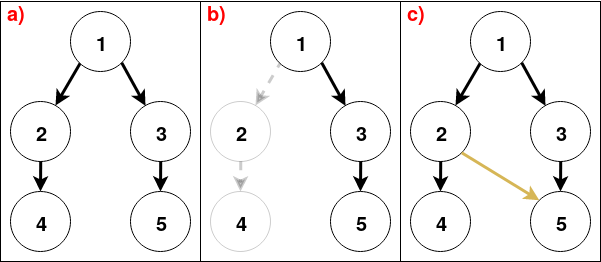
\includegraphics[scale=0.6]{Images/SoundAccurateGraph.png}
    %\caption[An example of soundness and accuracy in CFG:s.]{An example of soundness and accuracy in CFG:s. Graph a is the ideal CFG, graph b is an accurate approximation of the ideal CFG and graph c is a sound approximation of the ideal CFG. The transparent nodes andarrows denote unidentified parts of the graph. Yellow arrows denote falsely identified edges.}
    \label{fig:SoundAccurateGraph}
\end{figure}
\\ \\
Now, consider the three graphs from Figure \ref{fig:SoundAccurateGraph} again, depicted above for convenience. For graph b, denoted by $G_b$, the number of edges in the generated graph and the number of intersecting edges is 2. Consequently, the accuracy, soundness and precision for graph b evaluates to the values below. Note that the accuracy evaluates to 100\% and the graph is accurate since it does not contain any superfluous edges. 
\begin{center}
$\mathcal{A}_{E_I,E_{G_b}} = \frac{|E_I \cap E_{G_b}|}{|E_{G_b}|}=\frac{2}{2}=100\%$\\ $\mathcal{S}_{E_I,E_{G_b}} = \frac{|E_I \cap E_{G_b}|}{|E_I|}=\frac{2}{4}=50\%$\\
$ \mathcal{P}_{E_I,E_{G_b}} = \frac{\mathcal{A}_{E_I,E_{G_b}}+\mathcal{S}_{E_I,E_{G_b}}}{2}=\frac{1+0.5}{2}=75\%$\\
\end{center}
For graph c, which we denote by $G_c$, the amount of edges in the generated graph is 5 and the amount of intersecting edges is 4. Thus, the accuracy, soundness and precision for graph c becomes as presented in the equations below. For this graph, the soundness evaluates to 100\% and the graph is sound as it contains all edges of the ideal graph. 
\begin{center}
$\mathcal{A}_{E_I,E_{G_c}} = \frac{|E_I \cap E_{G_c}|}{|E_{G_c}|}=\frac{4}{5}=80\%$\\ $\mathcal{S}_{E_I,E_{G_c}} = \frac{|E_I \cap E_{G_c}|}{|E_I|}=\frac{4}{4}=100\%$\\
$ \mathcal{P}_{E_I,E_{G_c}} = \frac{\mathcal{A}_{E_I,E_{G_c}}+\mathcal{S}_{E_I,E_{G_c}}}{2}=\frac{0.8+1}{2}=90\%$\\
\end{center}
The calculations of the metrics presented above require the knowledge of which instructions a binary contains and the control flow transitions between these. True instructions and control flow transitions were determined through the use of angr. It should be noted that there are no guarantees that angr can find all instructions or that it won't accidentally announce data as instructions. However, determining the instructions of a program is as hard as determining the control flow of the program as they depend on each other. Consequently, this approach of approximating the ideal control flow with another state-of-the-art approach isn't an uncommon evaluation method\cite{preciseCFG}\cite{alternating}.
\\ \\
The evaluation proceeded as follows for each binary. First, our over/under-approximation algorithm was executed on the binary to produce a generated CFA. Thereafter, angr was executed to generate the, presumably ideal CFA. Finally, the accuracy, soundness and precision was generated for the generated CFA with and without top edges with respect to the ideal CFA, where top edges where defined as edges originating from a program location whose successors are unknown.

%See Section 5.1.1 and 5.1.3 in static analysis(?)
%Jakstab uses an SSL specification file
%Binary -(Dissassembly logic)> Assembly Instructions -> IR -> CFA Edges
%Fixed an off by one error
%Used socket instead of file because that avoids looks + messages can be queued
%Jakstab architecture Figure 5.1 in static analysis(if want to explain jakstab)
\section{Implementation}
\fbcomment{\color{red}Goal: Describe how Manticore was implemented (Considering to remove this section as I am not sure that is it "scientifically relevant")}
An illustration of the implementation is presented in Figure \ref{fig:implementationOverview}. Each node in the figure represent a module and each edge represents data transitioning between the components. The figure consists of one block representing Jakstab and one block representing Manticore. Our contributions consist of the ACFR algorithm in Jakstab and the two plugin modules developed for manticcore. Both of the plugin modules communicate intensively with Manticore's Symbolic Execution Engine which also communicates with other components which were omitted for simplicity. Additionally, some of the arrows for the Symbolic Execution Engine node have been omitted as they are not relevant for understanding our implementation.
\begin{figure}[!t]
    \centering
    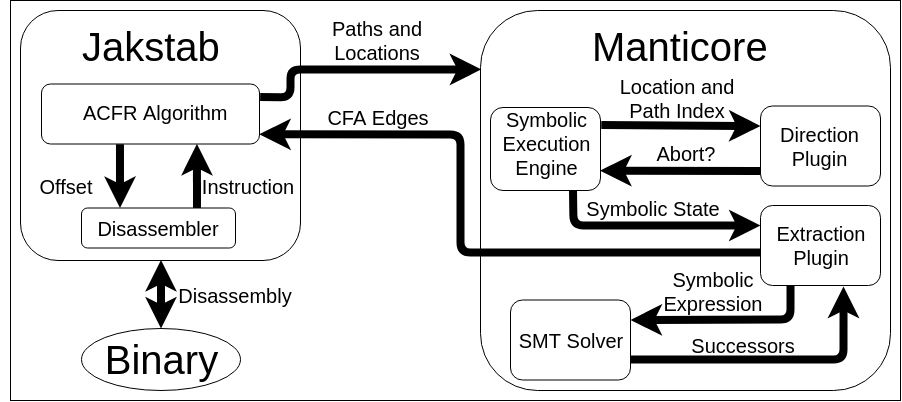
\includegraphics[scale=0.41]{Images/ImplementationOverview.png}
    \caption{An overview of the implementation.}
    \label{fig:implementationOverview}
\end{figure}
\\ \\
The process starts with the execution of the ACFR algorithm illustrated in the Jakstab box. The over-approximation conducts on demand disassembly to obtain instructions given an offset into the binary. The first offset is set to the program location that correspondds to the entrance of the binary and the subsequent offsets corresponds to the locations of subsequently obtained instructions. 
\\ \\
When the over-approximation stagnates, a limited depth first search is performed towards the unresolved program locations to obtain all possible paths starting at the program entrance and ending in these locations. The unresolved locations and paths are then sent to Manticore where they are used in the Direction Plugin and Extraction Plugin. The reasons for using plugins for Manticore, rather than editing the source code directly, was to enable compatibility for future versions of the software with our approach. For Jakstab, plugins were not possible due to the required modifications to the Jakstab algorithm.
\clearpage
\noindent
The Symbolic Execution Engine is started and informed about the plugins. Before each symbolic execution of an instruction, the Symbolic Execution Engine consults the Direction Plugin. This plugin receives the location of the instruction that is to be executed and the amount of instructions that were executed to reach the current instruction. The plugin then responds to the Symbolic Execution Engine if the location should be analyzed or not. This decision is performed according to the pseudo code in Figure \ref{fig:DSEupdate} presented in section \ref{sec:DSEPseudo}. 
\\ \\
After each analyzed symbolic state, the Symbolic Execution Engine sends the state to the Extraction Plugin which operates according to the pseudo code presented in Figure \ref{fig:DSEextract} introduced in section \ref{sec:DSEPseudo}. The extractor plugin checks if the state corresponds to the last location of any of the paths and that it has executed the instructions according to the path. If this is the case for any path, the plugin sends the symbolic expression for the next IP value to an SMT solver which responds with a set of possible successors. The plugin use these to create a set of CFA edges which aren't sent to Jakstab until the symbolic execution has completely terminated. Once the symbolic execution has completely terminated, the CFA edges are sent to Jakstab which adds them to the CFA and resumes the over-approximation
\section{Experiments}
\fbcomment{\color{red}Goal: Describe what experiments were done and why. Also, describe with enough details for the experiments to be reproducible}
We performed two sets of experiments. The first set of experiments were executed on our own synthetic benchmarks. The second set of experiments were performed on the five smallest GNU coreutils binaries. Due to Manticore's preference for statically linked binaries over dynamically linked binaries, all programs were linked statically. Furthermore, during our experiments, only one core was used as to reduce the effect of nondeterministic task scheduling on the results. 

%Manticore uses the Z3 SMT solver. DSE will benefit from the optimization of smt solvers.
%\subsection{Reproducibility}
\begin{figure}[ht]
\begin{tabular}{|ll|}
\hline
Architecture:   & x86\_64                                 \\ \hline
CPU op-modes: & 32-bit, 64-bit                            \\ \hline
CPU(s):         & 2                                       \\ \hline
Vendor ID:      & GenuineIntel                            \\ \hline
CPU family:     & 6                                       \\ \hline
CPU Model:      & 23                                      \\ \hline
CPU Model Name: & Pentium(R) Dual-Core CPU E5300@ 2.60GHz \\ \hline
RAM:            & 4GB                                     \\ \hline%4036412 kB
L1d cache:      & 32KB                                    \\ \hline
L1i cache:      & 32KB                                    \\ \hline
L2 cache:       & 2048KB                                  \\ \hline
\end{tabular}
\caption{Hardware specs of the host on which the experiments were performed.}
\label{fig:HWspecs}
\end{figure}
\noindent
\\ 
A fundamental problem in research, which is a great obstacle for the scientific method, is the difficulty in reproducing other researchers' results. This ongoing methodological crisis was originally coined as the "replication crisis"\cite{replicability}. As such, in this work, we aim to pay extra attention to provide the tools and information required for any scientist who desires to reproduce our results. 
\\ \\
The tool developed in this thesis is available online\footnote{\url{https://github.com/tpetersonkth/AlternatingControlFlowReconstruction}}. It was executed with python version 3.6.8, Manticore version 0.3.0 and java version 11.0.4. Jakstab was obtained from the original author online\footnote{\url{https://github.com/jkinder/jakstab}} and modified for our purposes. Furthermore, all input binaries were compiled into stripped and statically linked x86\_32 executables. The scripts for compiling input binaries, generating results and extracting metrics are all available online\footnote{\url{https://github.com/tpetersonkth/AlternatingControlFlowReconstruction/tree/thesis/utilities}}. As for the hardware, the relevant specs are provided in Figure \ref{fig:HWspecs}. More information concerning reproducibility is available in the wiki of the project\footnote{\url{https://github.com/tpetersonkth/AlternatingControlFlowReconstruction/wiki/Reproducibility}}.
\\ \\
For the experiments, we configured Manticore to assume a symbolic input from standard input with a maximum of 256 characters. Additionally, Manticore was configured for at most 3 arguments of 20 characters each. The reason for limiting the size of these input sources was to reduce the amount of required computation. Finally, Manticore was used with the SMT solver Z3 as this was the default SMT solver of the tool.
\\ \\
Originally, Manticore supported multithreaded symbolic execution. However, multithreading had to be disabled as a race condition bug was discovered\footnote{\url{https://github.com/trailofbits/Manticore/issues/1528}}. As such, all symbolic execution was performed using only one thread. We expect time spent performing DSE to be reduced by a constant factor when executed with multiple threads as multiple paths can be evaluated in parallell.
\\ \\

\chapter{Results}\label{chap:results}
\fbcomment{\color{red}Goal: Present the most "interesting" results of the project(Full tables will be put in an appendix).}
%The results achieved in the project are structured in a logical manner and clearly illustrated (tables, charts, etc.).
%Suitable data analysis or examination has been performed in a technically correct manner.
This chapter presents the results of our evaluations as well as the unplanned changes that had to be made to the strided interval domain of Jakstab. Initially, we present the changes that had to be made to the strided interval domain of Jakstab as it was essentially equivalent to the constant propagation domain due to an over-conservative widening operator. Therafter, we present the results of the evaluations of the synthetic binaries and the GNU coreutils binaries. Finally, a section is provided where the conclusions of the results are presented.
\\ \\
In the tables presented in this chapter, different abbreviations are used for different analysis modes. More specifically, c and i are used to denote constant propagation and strided interval analysis respectively. Furthermore, we let \it{cD} and \it{iD} denote constant propagation with DSE and strided interval analysis with DSE respectively.

%\section{Empirical Evaluations}
%Average Indirect Target Reduction (“Control Flow Integrity for COTS Binaries")
\clearpage
\section{Modifications to the Widening Operator of the Strided Interval Domain}
The original strided interval domain of Jakstab used an over-conservative widening operator. More specifically, when performing widening, it would always default to top unless the strided intervals represented the same value. Thus the original strided interval domain was essentially equivalent to the constant propagation domain since strided interval domains could only exists if they had a stride of $0$.
\\ \\
To be able to use intervals of other strides than $0$, we modified the widening operator to not over-approximate to $\top$ whenever two intervals did not have the same constant value. Rather, the widening operator was modified to combine the two strided intervals by creating a strided interval which did not include $\top$ unless necessary. Let $I_1=s_1[l_1,u_1]$ and $I_2=s_2[l_2,u_2]$ be two strided intervals. Furthermore, let $I_w=s_w[l_w,u_w]$ be the interval resulting from widening $I_1$ towards $I_2$. Then, $l_w$ and $u_w$ was defined as below. Note that $l_w$ is the minimum of the left bounds and $r_w$ is the maximum of the upper bounds.
\begin{center}
$l_w = l_1$ if $l_1 < l_2$, otherwise $l_2$\\
$r_w = r_1$ if $r_1 > r_2$, otherwise $r_2$
\end{center}
%The strided interval is an interval $s[l,u]=\{l + s * n\;|\;l \leq l + s * n \leq u, n \in \mathbb{N} \}$ where $s,l,u \in \mathbb{N}$ and $\mathbb{N}$ is the set of natural numbers including the zero element. 
For the stride $s_w$, however, things were more complicated as it needs to ensure that $I_w$ includes all elements of $I_1$ and $I_2$. This can essentially be broken down into two requirements. Firstly, $s_w$ must divide both $s_1$ and $s_2$. Secondly, $s_w$ must be set such that the lower bounds $l_1$ and $l_2$ are aligned. In essence, the second requirement can be phrased as $s_w \mid \lvert l_1-l_2 \rvert$. Now, let $gcd(x,y)$ be a function that returns the greatest common divisor of two integers $x$ and $y$ if $x\neq0$ and $y\neq0$. Otherwise, if one of the two parameters is zero, $gcd(x,y)$ returns the other parameter. We can now define the stride of the widened interval as follows:
\begin{center}
 $s_w = 
\begin{rcases}
    \begin{dcases}
        \lvert l_1-l_2 \rvert & \text{if}\;s_1 = 0\; \text{and} \; s_2 = 0\\
        gcd(gcd(s_1,s_2),\lvert l_1-l_2 \rvert) & \text{otherwise}
    \end{dcases}
\end{rcases}
$
\end{center}
By these definitions, it should be noted that the widening operator is symmetrical. In essence, widening $I_1$ towards $I_2$ or $I_2$ towards $I_1$ yields the same strided interval.

\section{Evaluation of Synthetic Binaries}\label{sec:synEval}
In this section we present the results of the synthetic evaluations. All of the synthetic binaries are available online\footnote{\url{https://github.com/tpetersonkth/AlternatingControlFlowReconstruction/tree/thesis/input/synthetic/bin}}. Thus, in this section, we will only describe the relevant part of the binaries for understanding our conclusions. Table \ref{tab:ACFR1Syn1} and \ref{tab:ACFR1Syn2} presents the results of executing the first version of ACFR on all synthetic binaries with a timeout of 2 hours and DFS depth of 200 instructions. The depth was set to 200 instructions as there might be loops in the binaries and thus, even if a binary only contains a small amount of instructions, there might be longer paths.
%Corresponds to /results/31OctDSEOnce
\begin{table}[!t]
\centering
\scalebox{0.5}{
\begin{tabular}{?l|l|l?l|l|l?l|l?l|l|l?l|l|l|l|l?}
\Xhline{2\arrayrulewidth}
\textbf{Binary} & \textbf{Mode} & \textbf{Instructions} & \textbf{$\mathcal{A}_{E_I,E_G}$} & \textbf{$\mathcal{P}_{E_I,E_G}$} & \textbf{$\mathcal{S}_{E_I,E_G}$} & \textbf{uTops} & \textbf{Tops} & \textbf{$\mathcal{A}_{E_I,E_{TF}}$} & \textbf{$\mathcal{P}_{E_I,E_{TF}}$} & \textbf{$\mathcal{S}_{E_I,E_{TF}}$} & \textbf{$T_{CPA}$} & \textbf{$T_{DFS}$} & \textbf{$T_{DSE}$} & \textbf{$T_{Other}$}\\ \Xhline{2\arrayrulewidth} 
badCall & c & 4 & 14.81\% & 40.74\% & 66.67\% & 1 & 1 & 100.0\% & 75.0\% & 50.0\% & 293ms & 0ms & 0ms & 113ms\\ \hline
badCall & cD & 7 & 20.0\% & 60.0\% & 100.0\% & 0 & 1 & 83.33\% & 83.33\% & 83.33\% & 264ms & 0ms & 680ms & 198ms\\ \hline
badCall & i & 7 & 85.71\% & 92.86\% & 100.0\% & 0 & 0 & 85.71\% & 92.86\% & 100.0\% & 256ms & 0ms & 0ms & 145ms\\ \hline
badCall & iD & 7 & 85.71\% & 92.86\% & 100.0\% & 0 & 0 & 85.71\% & 92.86\% & 100.0\% & 256ms & 0ms & 0ms & 216ms\\ \Xhline{2\arrayrulewidth} 
badIndMemJmp & c & 1 & 22.22\% & 44.44\% & 66.67\% & 1 & 1 & - & - & 0.0\% & 246ms & 0ms & 0ms & 127ms\\ \hline
badIndMemJmp & cD & 1 & 22.22\% & 44.44\% & 66.67\% & 0 & 1 & - & - & 0.0\% & 190ms & 0ms & 620ms & 201ms\\ \hline
badIndMemJmp & i & 1 & 0.0\% & 0.0\% & 0.0\% & 0 & 0 & 0.0\% & 0.0\% & 0.0\% & 103ms & 0ms & 0ms & 147ms\\ \hline
badIndMemJmp & iD & 1 & 0.0\% & 0.0\% & 0.0\% & 0 & 0 & 0.0\% & 0.0\% & 0.0\% & 89ms & 0ms & 0ms & 211ms\\ \Xhline{2\arrayrulewidth} 
branch & c & 17 & 20.45\% & 60.23\% & 100.0\% & 1 & 1 & 94.12\% & 91.5\% & 88.89\% & 323ms & 0ms & 0ms & 123ms\\ \hline
branch & cD & 17 & 20.45\% & 60.23\% & 100.0\% & 0 & 1 & 94.12\% & 91.5\% & 88.89\% & 463ms & 1ms & 684ms & 204ms\\ \hline
branch & i & 17 & 94.74\% & 97.37\% & 100.0\% & 0 & 0 & 94.74\% & 97.37\% & 100.0\% & 471ms & 0ms & 0ms & 119ms\\ \hline
branch & iD & 17 & 94.74\% & 97.37\% & 100.0\% & 0 & 0 & 94.74\% & 97.37\% & 100.0\% & 474ms & 0ms & 0ms & 210ms\\ \Xhline{2\arrayrulewidth} 
callRet & c & 2 & 8.33\% & 24.17\% & 40.0\% & 1 & 1 & 100.0\% & 60.0\% & 20.0\% & 266ms & 0ms & 0ms & 136ms\\ \hline
callRet & cD & 6 & 17.86\% & 58.93\% & 100.0\% & 0 & 1 & 80.0\% & 80.0\% & 80.0\% & 267ms & 3ms & 657ms & 208ms\\ \hline
callRet & i & 6 & 83.33\% & 91.67\% & 100.0\% & 0 & 0 & 83.33\% & 91.67\% & 100.0\% & 254ms & 0ms & 0ms & 148ms\\ \hline
callRet & iD & 6 & 83.33\% & 91.67\% & 100.0\% & 0 & 0 & 83.33\% & 91.67\% & 100.0\% & 250ms & 0ms & 0ms & 213ms\\ \Xhline{2\arrayrulewidth} 
cjmp & c & 11 & 90.91\% & 95.45\% & 100.0\% & 0 & 0 & 90.91\% & 95.45\% & 100.0\% & 291ms & 0ms & 0ms & 127ms\\ \hline
cjmp & cD & 11 & 90.91\% & 95.45\% & 100.0\% & 0 & 0 & 90.91\% & 95.45\% & 100.0\% & 290ms & 0ms & 0ms & 203ms\\ \hline
cjmp & i & 11 & 90.91\% & 95.45\% & 100.0\% & 0 & 0 & 90.91\% & 95.45\% & 100.0\% & 279ms & 0ms & 0ms & 173ms\\ \hline
cjmp & iD & 11 & 90.91\% & 95.45\% & 100.0\% & 0 & 0 & 90.91\% & 95.45\% & 100.0\% & 269ms & 0ms & 0ms & 252ms\\ \Xhline{2\arrayrulewidth} 
cjmpBitOp & c & 7 & 85.71\% & 92.86\% & 100.0\% & 0 & 0 & 85.71\% & 92.86\% & 100.0\% & 277ms & 0ms & 0ms & 122ms\\ \hline
cjmpBitOp & cD & 7 & 85.71\% & 92.86\% & 100.0\% & 0 & 0 & 85.71\% & 92.86\% & 100.0\% & 278ms & 0ms & 0ms & 194ms\\ \hline
cjmpBitOp & i & 8 & 75.0\% & 87.5\% & 100.0\% & 0 & 0 & 75.0\% & 87.5\% & 100.0\% & 267ms & 0ms & 0ms & 142ms\\ \hline
cjmpBitOp & iD & 8 & 75.0\% & 87.5\% & 100.0\% & 0 & 0 & 75.0\% & 87.5\% & 100.0\% & 252ms & 0ms & 0ms & 214ms\\ \Xhline{2\arrayrulewidth} 
conditionalTop & c & 11 & 33.33\% & 66.67\% & 100.0\% & 1 & 1 & 100.0\% & 78.95\% & 57.89\% & 303ms & 0ms & 0ms & 129ms\\ \hline
conditionalTop & cD & 11 & 33.33\% & 66.67\% & 100.0\% & 0 & 1 & 100.0\% & 78.95\% & 57.89\% & 285ms & 1ms & 766ms & 211ms\\ \hline
conditionalTop & i & 11 & 33.33\% & 66.67\% & 100.0\% & 1 & 1 & 100.0\% & 78.95\% & 57.89\% & 312ms & 0ms & 0ms & 136ms\\ \hline
conditionalTop & iD & 11 & 33.33\% & 66.67\% & 100.0\% & 0 & 1 & 100.0\% & 78.95\% & 57.89\% & 277ms & 1ms & 896ms & 241ms\\ \Xhline{2\arrayrulewidth} 
doubleCallRet & c & 17 & 9.47\% & 45.65\% & 81.82\% & 2 & 2 & 100.0\% & 86.36\% & 72.73\% & 304ms & 0ms & 0ms & 149ms\\ \hline
doubleCallRet & cD & 22 & 11.28\% & 55.64\% & 100.0\% & 0 & 2 & 95.24\% & 93.07\% & 90.91\% & 301ms & 0ms & 794ms & 223ms\\ \hline
doubleCallRet & i & 22 & 95.65\% & 97.83\% & 100.0\% & 0 & 0 & 95.65\% & 97.83\% & 100.0\% & 287ms & 0ms & 0ms & 166ms\\ \hline
doubleCallRet & iD & 22 & 95.65\% & 97.83\% & 100.0\% & 0 & 0 & 95.65\% & 97.83\% & 100.0\% & 288ms & 0ms & 0ms & 238ms\\ \Xhline{2\arrayrulewidth} 
espAssignment & c & 9 & 16.33\% & 58.16\% & 100.0\% & 1 & 1 & 87.5\% & 87.5\% & 87.5\% & 324ms & 0ms & 0ms & 124ms\\ \hline
espAssignment & cD & 9 & 16.33\% & 58.16\% & 100.0\% & 1 & 1 & 87.5\% & 87.5\% & 87.5\% & 277ms & 4ms & 528ms & 343ms\\ \hline
espAssignment & i & 9 & 16.33\% & 58.16\% & 100.0\% & 1 & 1 & 87.5\% & 87.5\% & 87.5\% & 326ms & 0ms & 0ms & 129ms\\ \hline
espAssignment & iD & 9 & 16.33\% & 58.16\% & 100.0\% & 1 & 1 & 87.5\% & 87.5\% & 87.5\% & 273ms & 13ms & 558ms & 361ms\\ \Xhline{2\arrayrulewidth} 
indMemJmp & c & 6 & 83.33\% & 91.67\% & 100.0\% & 0 & 0 & 83.33\% & 91.67\% & 100.0\% & 269ms & 0ms & 0ms & 123ms\\ \hline
indMemJmp & cD & 6 & 83.33\% & 91.67\% & 100.0\% & 0 & 0 & 83.33\% & 91.67\% & 100.0\% & 261ms & 0ms & 0ms & 196ms\\ \hline
indMemJmp & i & 6 & 83.33\% & 91.67\% & 100.0\% & 0 & 0 & 83.33\% & 91.67\% & 100.0\% & 255ms & 0ms & 0ms & 138ms\\ \hline
indMemJmp & iD & 6 & 83.33\% & 91.67\% & 100.0\% & 0 & 0 & 83.33\% & 91.67\% & 100.0\% & 239ms & 0ms & 0ms & 228ms\\ \Xhline{2\arrayrulewidth} 
infiniteLoop & c & 10 & 66.67\% & 83.33\% & 100.0\% & 0 & 0 & 66.67\% & 83.33\% & 100.0\% & 310ms & 0ms & 0ms & 127ms\\ \hline
infiniteLoop & cD & 10 & 66.67\% & 83.33\% & 100.0\% & 0 & 0 & 66.67\% & 83.33\% & 100.0\% & 287ms & 0ms & 0ms & 205ms\\ \hline
infiniteLoop$\triangle_{T}$ & i & 10 & 66.67\% & 83.33\% & 100.0\% & 0 & 0 & 66.67\% & 83.33\% & 100.0\% & 7141883ms & 0ms & 0ms & 63ms\\ \hline
infiniteLoop$\triangle_{T}$ & iD & 10 & 66.67\% & 83.33\% & 100.0\% & 0 & 0 & 66.67\% & 83.33\% & 100.0\% & 7141893ms & 0ms & 0ms & 105ms\\ \Xhline{2\arrayrulewidth} 
int & c & 9 & 88.89\% & 94.44\% & 100.0\% & 0 & 0 & 88.89\% & 94.44\% & 100.0\% & 257ms & 0ms & 0ms & 138ms\\ \hline
int & cD & 9 & 88.89\% & 94.44\% & 100.0\% & 0 & 0 & 88.89\% & 94.44\% & 100.0\% & 265ms & 0ms & 0ms & 190ms\\ \hline
int & i & 9 & 88.89\% & 94.44\% & 100.0\% & 0 & 0 & 88.89\% & 94.44\% & 100.0\% & 239ms & 0ms & 0ms & 141ms\\ \hline
int & iD & 9 & 88.89\% & 94.44\% & 100.0\% & 0 & 0 & 88.89\% & 94.44\% & 100.0\% & 233ms & 0ms & 0ms & 216ms\\ \Xhline{2\arrayrulewidth} 
kindConditionalTop & c & 8 & 26.83\% & 63.41\% & 100.0\% & 1 & 1 & 100.0\% & 81.82\% & 63.64\% & 285ms & 0ms & 0ms & 120ms\\ \hline
kindConditionalTop & cD & 8 & 26.83\% & 63.41\% & 100.0\% & 0 & 1 & 100.0\% & 81.82\% & 63.64\% & 282ms & 0ms & 659ms & 190ms\\ \hline
kindConditionalTop & i & 8 & 26.83\% & 63.41\% & 100.0\% & 1 & 1 & 100.0\% & 81.82\% & 63.64\% & 306ms & 0ms & 0ms & 116ms\\ \hline
kindConditionalTop & iD & 8 & 26.83\% & 63.41\% & 100.0\% & 0 & 1 & 100.0\% & 81.82\% & 63.64\% & 250ms & 1ms & 694ms & 234ms\\ \Xhline{2\arrayrulewidth}
\end{tabular}
}
\caption[Results of the synthetic benchmarks for the first version of the ACFR algorithm (Part 1).]{Results of the synthetic benchmarks for the first version of the ACFR algorithm (Part 1). Analyses which had to be interrupted as they did not finish within 2 hours are marked with  $\triangle_{T}$.}
\label{tab:ACFR1Syn1}
\end{table}
\\ \\
%\noindent
The first column of the tables denotes the name of the binary. Then, the second is the analysis mode that was used. Here, \it{c} and \it{i} signifies constant propagation and strided intervals respectively. Further, a \it{D} signifies that the analysis was executed with DSE. The third column is the number of identified instructions. Thereafter, the next three columns are the accuracy, precision and soundness of the generated graph with respect to the manually reconstructed ideal graph. 
\\ \\
Thereafter, \textbf{uTops} and \textbf{Tops} denote the number of unresolved tops and total amount of Tops. Note that an unresolved top is defined as a top where no successor could be determined. As such, a top which have multiple successors where only one of these could be determined, is not considered as an unresolved top. The top stats are followed by three columns which are the accuracy, precision and soundness of the top-free version of the generated graph with respect to the manually reconstructed ideal graph. Finally, the last four columns show the time spent executing the over-approximation, DFS, DSE and time spent executing everything outside of these three components. 
\\ \\
The first binary, \it{badCall}, contains a push to the stack with a return address and a jump to a location with a \it{ret} instruction. Thus, a call is performed without using the \it{call} instruction. As can be seen in the table, the constant propagation could only resolve the instructions up to the \it{ret} instructions since it does not assume any initial stack value. However, with the help of DSE, constant propagation was able reconstruct a sound CFA. Note, however, that the top-free generated graph did not include the edge from the resolved top to it's successor and thus the graph could not achieve 100\% soundness. On the other hand, the top-free version had a higher precision since the reconstructed CFA was accurate. Finally, the interval domain didn't encounter any tops and thus didn't need to use DSE.
%Maybe this binary is not jumping to the content of the address..
\clearpage
\noindent
The next binary is \it{badIndMemJmp} which only contains one indirect jump to an uninitialized memory location and three instructions to perform a sys exit. The indirect jump is a true top and the successors of the instructions can thus be any instruction in the text section.  What is peculiar about the analyses based on constant propagation is that their top free version of the CFA does not contain any edges and thus has an undefined accuracy as well as precision. Furthermore, the interval analysis claimed that a successor of the indirect jump could be a location outside the text section. Consequently, the CFAs from the strided intervals did not have any intersecting edges with the ideal graph and thus had 0\% for all metrics.
\begin{table}[!t]
\centering
\scalebox{0.5}{
\begin{tabular}{?l|l|l?l|l|l?l|l?l|l|l?l|l|l|l|l?}
\Xhline{2\arrayrulewidth}
\textbf{Binary} & \textbf{Mode} & \textbf{Instructions} & \textbf{$\mathcal{A}_{E_I,E_G}$} & \textbf{$\mathcal{P}_{E_I,E_G}$} & \textbf{$\mathcal{S}_{E_I,E_G}$} & \textbf{uTops} & \textbf{Tops} & \textbf{$\mathcal{A}_{E_I,E_{TF}}$} & \textbf{$\mathcal{P}_{E_I,E_{TF}}$} & \textbf{$\mathcal{S}_{E_I,E_{TF}}$} & \textbf{$T_{CPA}$} & \textbf{$T_{DFS}$} & \textbf{$T_{DSE}$} & \textbf{$T_{Other}$}\\ \Xhline{2\arrayrulewidth} 
longRegisterEquals & c & 14 & 15.38\% & 57.69\% & 100.0\% & 1 & 1 & 66.67\% & 83.33\% & 100.0\% & 315ms & 0ms & 0ms & 119ms\\ \hline
longRegisterEquals & cD & 14 & 15.38\% & 57.69\% & 100.0\% & 1 & 1 & 66.67\% & 83.33\% & 100.0\% & 302ms & 0ms & 702ms & 189ms\\ \hline
longRegisterEquals & i & 14 & 15.38\% & 57.69\% & 100.0\% & 1 & 1 & 66.67\% & 83.33\% & 100.0\% & 319ms & 0ms & 0ms & 142ms\\ \hline
longRegisterEquals & iD & 14 & 15.38\% & 57.69\% & 100.0\% & 1 & 1 & 66.67\% & 83.33\% & 100.0\% & 266ms & 1ms & 559ms & 219ms\\ \Xhline{2\arrayrulewidth} 
memCallRet & c & 4 & 10.53\% & 33.83\% & 57.14\% & 1 & 1 & 100.0\% & 71.43\% & 42.86\% & 287ms & 0ms & 0ms & 116ms\\ \hline
memCallRet & cD & 8 & 16.67\% & 58.33\% & 100.0\% & 0 & 1 & 85.71\% & 85.71\% & 85.71\% & 285ms & 1ms & 589ms & 196ms\\ \hline
memCallRet & i & 8 & 87.5\% & 93.75\% & 100.0\% & 0 & 0 & 87.5\% & 93.75\% & 100.0\% & 261ms & 0ms & 0ms & 141ms\\ \hline
memCallRet & iD & 8 & 87.5\% & 93.75\% & 100.0\% & 0 & 0 & 87.5\% & 93.75\% & 100.0\% & 255ms & 0ms & 0ms & 224ms\\ \Xhline{2\arrayrulewidth} 
minimalistic & c & 5 & 10.71\% & 20.36\% & 30.0\% & 1 & 1 & 100.0\% & 60.0\% & 20.0\% & 276ms & 0ms & 0ms & 132ms\\ \hline
minimalistic & cD & 11 & 19.35\% & 39.68\% & 60.0\% & 0 & 1 & 100.0\% & 75.0\% & 50.0\% & 280ms & 0ms & 632ms & 215ms\\ \hline
minimalistic & i & 11 & 19.35\% & 39.68\% & 60.0\% & 1 & 1 & 100.0\% & 75.0\% & 50.0\% & 328ms & 0ms & 0ms & 132ms\\ \hline
minimalistic $\triangle_{T}$ & iD & 15 & 13.68\% & 46.84\% & 80.0\% & 1 & 2 & 100.0\% & 82.5\% & 65.0\% & 7148928ms & 9ms & 626ms & 291ms\\ \Xhline{2\arrayrulewidth} 
nestedCallRet & c & 3 & 9.68\% & 26.27\% & 42.86\% & 1 & 1 & 100.0\% & 64.29\% & 28.57\% & 272ms & 0ms & 0ms & 122ms\\ \hline
nestedCallRet & cD & 8 & 10.94\% & 55.47\% & 100.0\% & 0 & 2 & 83.33\% & 77.38\% & 71.43\% & 270ms & 1ms & 1160ms & 199ms\\ \hline
nestedCallRet & i & 8 & 87.5\% & 93.75\% & 100.0\% & 0 & 0 & 87.5\% & 93.75\% & 100.0\% & 260ms & 0ms & 0ms & 154ms\\ \hline
nestedCallRet & iD & 8 & 87.5\% & 93.75\% & 100.0\% & 0 & 0 & 87.5\% & 93.75\% & 100.0\% & 238ms & 0ms & 0ms & 231ms\\ \Xhline{2\arrayrulewidth} 
registerEquals & c & 8 & 15.15\% & 57.58\% & 100.0\% & 1 & 1 & 62.5\% & 81.25\% & 100.0\% & 301ms & 0ms & 0ms & 127ms\\ \hline
registerEquals & cD & 8 & 15.15\% & 57.58\% & 100.0\% & 1 & 1 & 62.5\% & 81.25\% & 100.0\% & 285ms & 1ms & 605ms & 214ms\\ \hline
registerEquals & i & 8 & 15.15\% & 57.58\% & 100.0\% & 1 & 1 & 62.5\% & 81.25\% & 100.0\% & 299ms & 0ms & 0ms & 122ms\\ \hline
registerEquals & iD & 8 & 15.15\% & 57.58\% & 100.0\% & 1 & 1 & 62.5\% & 81.25\% & 100.0\% & 261ms & 3ms & 761ms & 230ms\\ \Xhline{2\arrayrulewidth} 
sequentialCallRet & c & 2 & 10.34\% & 26.6\% & 42.86\% & 1 & 1 & 100.0\% & 57.14\% & 14.29\% & 276ms & 0ms & 0ms & 133ms\\ \hline
sequentialCallRet & cD & 3 & 13.33\% & 35.24\% & 57.14\% & 0 & 1 & 100.0\% & 64.29\% & 28.57\% & 258ms & 0ms & 773ms & 188ms\\ \hline
sequentialCallRet & i & 7 & 87.5\% & 93.75\% & 100.0\% & 0 & 0 & 87.5\% & 93.75\% & 100.0\% & 271ms & 0ms & 0ms & 167ms\\ \hline
sequentialCallRet & iD & 7 & 87.5\% & 93.75\% & 100.0\% & 0 & 0 & 87.5\% & 93.75\% & 100.0\% & 260ms & 0ms & 0ms & 231ms\\ \Xhline{2\arrayrulewidth} 
stackBO & c & 13 & 37.23\% & 59.31\% & 81.4\% & 1 & 1 & 100.0\% & 63.95\% & 27.91\% & 303ms & 0ms & 0ms & 138ms\\ \hline
stackBO & cD & 13 & 37.23\% & 59.31\% & 81.4\% & 0 & 1 & 100.0\% & 63.95\% & 27.91\% & 291ms & 0ms & 933ms & 210ms\\ \hline
stackBO & i & 22 & 95.45\% & 72.15\% & 48.84\% & 0 & 0 & 95.45\% & 72.15\% & 48.84\% & 281ms & 0ms & 0ms & 151ms\\ \hline
stackBO & iD & 22 & 95.45\% & 72.15\% & 48.84\% & 0 & 0 & 95.45\% & 72.15\% & 48.84\% & 278ms & 0ms & 0ms & 232ms\\ \Xhline{2\arrayrulewidth} 
trueTop & c & 7 & 34.29\% & 67.14\% & 100.0\% & 1 & 1 & 100.0\% & 75.0\% & 50.0\% & 291ms & 0ms & 0ms & 132ms\\ \hline
trueTop & cD & 7 & 34.29\% & 67.14\% & 100.0\% & 0 & 1 & 100.0\% & 75.0\% & 50.0\% & 273ms & 1ms & 1053ms & 201ms\\ \hline
trueTop & i & 7 & 34.29\% & 67.14\% & 100.0\% & 1 & 1 & 100.0\% & 75.0\% & 50.0\% & 289ms & 0ms & 0ms & 125ms\\ \hline
trueTop & iD & 7 & 34.29\% & 67.14\% & 100.0\% & 0 & 1 & 100.0\% & 75.0\% & 50.0\% & 261ms & 1ms & 810ms & 222ms\\ \Xhline{2\arrayrulewidth} 
twoVars & c & 7 & 18.37\% & 46.68\% & 75.0\% & 1 & 1 & 100.0\% & 79.17\% & 58.33\% & 305ms & 0ms & 0ms & 137ms\\ \hline
twoVars & cD & 11 & 22.64\% & 61.32\% & 100.0\% & 0 & 1 & 90.91\% & 87.12\% & 83.33\% & 278ms & 0ms & 632ms & 210ms\\ \hline
twoVars & i & 7 & 18.37\% & 46.68\% & 75.0\% & 1 & 1 & 100.0\% & 79.17\% & 58.33\% & 305ms & 0ms & 0ms & 140ms\\ \hline
twoVars & iD & 11 & 22.64\% & 61.32\% & 100.0\% & 0 & 1 & 90.91\% & 87.12\% & 83.33\% & 247ms & 1ms & 652ms & 268ms\\ \Xhline{2\arrayrulewidth} 
xyz & c & 10 & 16.95\% & 50.14\% & 83.33\% & 1 & 1 & 100.0\% & 87.5\% & 75.0\% & 299ms & 0ms & 0ms & 139ms\\ \hline
xyz & cD & 13 & 19.35\% & 59.68\% & 100.0\% & 0 & 1 & 91.67\% & 91.67\% & 91.67\% & 290ms & 1ms & 742ms & 218ms\\ \hline
xyz & i & 10 & 16.95\% & 50.14\% & 83.33\% & 1 & 1 & 100.0\% & 87.5\% & 75.0\% & 309ms & 0ms & 0ms & 112ms\\ \hline
xyz & iD & 13 & 19.35\% & 59.68\% & 100.0\% & 0 & 1 & 91.67\% & 91.67\% & 91.67\% & 262ms & 9ms & 753ms & 220ms\\ \Xhline{2\arrayrulewidth}
\end{tabular}
}
\caption[Results of the synthetic benchmarks for the first version of the ACFR algorithm (Part 2).]{Results of the synthetic benchmarks for the first version of the ACFR algorithm (Part 2). Analyses which had to be interrupted as they did not finish within 2 hours are marked with $\triangle_{T}$.}
\label{tab:ACFR1Syn2}
\end{table}
\\ \\
The \it{branch} binary corresponds to the assembly code presented in section \ref{sec:absDomInt}. For this binary, the constant propagation based analyses generated a CFA which was sound but whose top-free version was unsound since it excluded all edges from top nodes. Furthermore, Something interesting to note about the constant propagation analysis is that it had the same accuracy, precision and soundness independently of if it took help from DSE even though a top was resolved when DSE was used. 
\\ \\
DSE contributed with one extra top edge which, however, did not increase the precision since Jakstab can not know if the new set of edges is an over-approximation of the true edges from the top node and thus still must include one edge from the top node to each other program location. Furthermore, for the strided interval analysis, there were no tops and thus no difference between when DSE was used and not used, Additionally, the precision was fairly high compared to the precision achieved for other binaries. The reason that a CFA with a precision of 100\% was not reconstructed was that one edge was falsely identified as being part of the CFA.
\\ \\
The fourth binary is \it{callRet} which is a binary containing a simple function call and return statement. Similarly to the \it{badCall} binary, constant propagation could not resolve the \it{ret} instruction since it does not assume an initial \it{esp} value. Thereafter, the subsequent binary corresponds to the example illustrating the capabilities of constant propagation in section \ref{sec:absDomCon}. For this binary, there were no tops and all modes resulted in the same CFA.
\\ \\
Afterwards, the analysis of the \it{cjmpBitOp} binary suggests that constant propagation can be more accurate than strided intervals. This binary contains a \it{je} instruction which jumps if the result of a previous \it{cmp} resulted in equality between to registers. The comparision compared two equal values and the \it{je} instruction should thus always result in a jump. However,one of the registers that were compared was shifted before the comparison. This proved to be a problem for the interval domain which over-approximated the new value of the register while the constant propagation could handle the shifting without over-approximation.
\clearpage
\noindent
The next binary, \it{conditionalTop}, didn't exhibit any significant differences between the analysis modes. Furthermore, the \it{doubleCallRet} binary did not show anything particular except that constant propagation needed DSE to handle \it{ret} instrucitons as had already been determined. Thereafter, the \it{espAssignment}, \it{indMemJump}, \it{infiniteLoop}, \it{int}, \it{kindConditionalTop} and \it{longRegisterEquals} binaries didn't show any significant variation between the analysis modes. However, during the analysis of \it{infiniteLoop}, the interval timed out after 2 hours. The reason for this timeout was a loop in the reconstructed CFA which had a unequal number of \it{call} and \it{ret} instructions. As a consequence, the strided interval of the \it{esp} register was decreased by 4 byte for each iteration of the loop. Thus, the analysis could not reach a fixpoint. This limitation of the strided interval domain will be explained in further detail in section \ref{sec:conclusions}.
\\ \\ 
The subsequent binaries; \it{memCallRet}, \it{minimalistic}, \it{nestedCallRet} and \it{registerEquals}, did not exhibit anything out of the ordinary concerning precision apart from constant propagation's dependence on DSE. Hwever, by looking at the benchmarking columns, we can determine that \it{minimalistic} timed out at 2 hours in mode \it{iD}. The reason was the same as for the \it{infiniteLoop} binary presented earlier. Note, however, that the timeout only occured when the strided interval domain was combined with DSE. From the log files of our experiments, we could determine that the problem was not explicitly caused by DSE. Rather, DSE contributed with an edge that permitted the analysis to continue and incorrectly identify a cycle with a unequal number of \it{call} and \it{ret} instructions at a later point. 
\\ \\
For the next two binaries, \it{sequentialCallRet} and \it{stackBO}, it can be observed that the strided interval domain based analysis had a higher precision than the constant propagation based analysis both with and without DSE. The former binary corresponds to the third example in section \ref{sec:MotExamples} and contains two calls to one function in sequence. For constant propagation with DSE and the first version of the ACFR algortihm, the successors of the \it{ret} instruction are only requested once. As such the analysis with the \it{cD} mode could not achieve 100\% soundness for the generated graph like the strided interval domain.
\clearpage
\noindent   
For the latter binary, \it{stackBo}, the constant propagation based analyses had higher soundness than those based on the strided interval analysis. This binary contains a function vulnerable to a stack buffer overflow which can overflow the return pointer, located on the stack, with an arbitrary value. By comparing the soundness of the original version of the generated graph and the top-free version for the constant propagation based analyses, it can clearly be seen that the top-edges contributed significantly to the soundness of the graph. 
\\ \\
This was because the only top was located at the \it{ret} instruction in the vulnerable function and thus this top is actually a true top since the return pointer can be arbitrarily modified. Furthermore, as the buffer overflow violates the assumptions of Jakstab, the interval domain claims that no tops were discovered. Finally, Since the precision for this binary over all analysis modes is not significantly bad, one could argue that Jakstab could still be useful for binaries which violates its assumptions.
\\ \\
The next binary, \it{trueTop}, which corresponds to the example in section \ref{fig:trueTop.asm}, had no differences between the CFA:s over the different analysis modes. Finally, the last two binaries, \it{twoVars} and \it{xyz}(Which corresponds to the example in section \ref{sec:MotExamples}), have an increase of precision when using DSE for both of the abstract domains. This shows that there are cases which can not be evaluated with any of the two abstract domains but can be handled with DSE.

%Corresponds to /results/31Oct
\begin{table}[!t]
\centering
\scalebox{0.5}{
\begin{tabular}{?l|l|l?l|l|l?l|l?l|l|l?l|l|l|l|l?}
\Xhline{2\arrayrulewidth}
\textbf{Binary} & \textbf{Mode} & \textbf{Instructions} & \textbf{$\mathcal{A}_{E_I,E_G}$} & \textbf{$\mathcal{P}_{E_I,E_G}$} & \textbf{$\mathcal{S}_{E_I,E_G}$} & \textbf{uTops} & \textbf{Tops} & \textbf{$\mathcal{A}_{E_I,E_{TF}}$} & \textbf{$\mathcal{P}_{E_I,E_{TF}}$} & \textbf{$\mathcal{S}_{E_I,E_{TF}}$} & \textbf{$T_{CPA}$} & \textbf{$T_{DFS}$} & \textbf{$T_{DSE}$} & \textbf{$T_{Other}$}\\ \Xhline{2\arrayrulewidth} 
minimalistic & c & 5 & 10.71\% & 20.36\% & 30.0\% & 1 & 1 & 100.0\% & 60.0\% & 20.0\% & 268ms & 0ms & 0ms & 146ms\\ \hline
minimalistic & cD & 35 & 10.53\% & 55.26\% & 100.0\% & 0 & 3 & 47.06\% & 63.53\% & 80.0\% & 574ms & 44ms & 4615ms & 725ms\\ \hline
minimalistic & i & 11 & 19.35\% & 39.68\% & 60.0\% & 1 & 1 & 100.0\% & 75.0\% & 50.0\% & 365ms & 0ms & 0ms & 130ms\\ \hline
minimalistic$\triangle_{T}$ & iD & 15 & 13.68\% & 46.84\% & 80.0\% & 1 & 2 & 100.0\% & 82.5\% & 65.0\% & 7148204ms & 7ms & 686ms & 293ms\\ \Xhline{2\arrayrulewidth} 
sequentialCallRet & c & 2 & 10.34\% & 26.6\% & 42.86\% & 1 & 1 & 100.0\% & 57.14\% & 14.29\% & 269ms & 0ms & 0ms & 121ms\\ \hline
sequentialCallRet & cD & 7 & 20.59\% & 60.29\% & 100.0\% & 0 & 1 & 83.33\% & 77.38\% & 71.43\% & 277ms & 22ms & 3644ms & 655ms\\ \hline
sequentialCallRet & i & 7 & 87.5\% & 93.75\% & 100.0\% & 0 & 0 & 87.5\% & 93.75\% & 100.0\% & 271ms & 0ms & 0ms & 150ms\\ \hline
sequentialCallRet & iD & 7 & 87.5\% & 93.75\% & 100.0\% & 0 & 0 & 87.5\% & 93.75\% & 100.0\% & 264ms & 0ms & 0ms & 222ms\\ \Xhline{2\arrayrulewidth} 
\end{tabular}
}
\caption[Results of the synthetic benchmarks for the second version of the ACFR algorithm (Part 2).]{Results of the synthetic benchmarks for the second version of the ACFR algorithm which differed from the results obtained with the first version. Analyses which had to be interrupted as they did not finish within 2 hours are marked with $\triangle_{T}$.}
\label{tab:ACFR2SynDiff}
\end{table}
\noindent
\\
The results of the analysis of synthetic binaries using the second version of the ACFR algorithm can be observed in Table \ref{tab:ACFR2SynDiff}. This table only includes the two binaries which had a different precision when executed with the second version compared to the first version of the algorithm\footnote{The full table can be found in appendix A.}. The results of the second version of the algorithm is very similar to the first. In fact, the only time the analyses did not reconstruct the same CFA as the first version was for the  \it{sequentialCallRet} and \it{minimalistic}. As the former binary was the example of why the second algorithm was better than the first, illustrated in section \ref{sec:MotExamples}, this should not appear as a surprise. The second binary was a minimalistical c program compiled statically without stdlib. For this binary, the soundness of the CFA resulting from the \it{cD} mode increased for the top-including CFA from 60\% to 100\%.
\\ \\
Furthermore, for the top-free CFA, the soundness increased from 50\% to 80\% in this mode. However, due to a lot of false positives, the accuracy decreased by 8.82 and 52.94 percentage points for the top-including and top-free CFA respectively. This resulted in the somewhat strange result that the usage of the second version of ACFR created a CFA which was more precise when including top edges but less precise when excluding top edges. From the precision uncertainties, we can see that the second version of the ACFR algorirthm does not guarantee an increase in precision. Rather, it guarantees the soundness to be equal or higher than the soundness resulting from the usage of the first version of the algorihtm.
\\ \\
Another somewhat surprising aspect concerning the analysis of this binary is that the constant propagation with DSE identified 35 instructions while only 11 instructions actually existed in the binary. The \it{minimalistic} binary was compiled without the c standard library and with the main method set as the entry point of the binary. As such, the binary ended with a \it{ret} instruction which should not have any well-defined successors. However, when the over-approximation reached this instruction, it asked DSE for a possible successor which was then provided. The over-approximation then progressed by disassembling instructions at the new location, continuing to ask for successors of any encountered tops. This proceeded until the analysis reached a sequence of bytes which did not correspond to an instruction.
\\ \\
Note that one could possibly argue that the manually reconstructed CFA was wrong since it is actually possible to execute the last \it{ret} instruction. Furthermore, one could then argue that the preciseness of the reconstructed CFA using the \it{cD} mode would be higher than the other modes. However, we chose to limit out definition of the ideal control flow to instructions with well-defined behaviour. 
%TODO introduce top-including and top-free graph earlier. (Think top-edge-free graph and so on)
\section{Evaluation of GNU Coreutils}\label{sec:evalGNU}
Due to a limited amount of computational resources, the evaluation was limited to the 5 smallest GNU coreutils binaries. The results of the evalutions using the first version of ACFR are presented in Table \ref{tab:ACFR1GNUCoreutils}. The results of the evaluation using the second version of ACFR did not differ in accuracy, soundness or precision for any of the binaries and are thus not presented.
\\ \\
As could have been expected, the constant propagation finished quickly but was not useful on its own, only managing to identify the first 10 instruction of each binary. However, with the help of DSE, constant propagation was able to increase the soundness of the reconstructed CFA. On the other hand, during the extraction of possible paths for DSE, the analysis had an out of memory exception. We believe that this occured because of the large amount of possible paths due to loops in the CFA. More specifically, for each loop, one path exists for each iteration of the loop. Additionally, if loops are nested, the number of paths can be significantly larger, as will be explained in section \ref{sec:numPaths}.
\\ \\
As can be seen in the table, for each binary, analyses based on the strided interval did not finish within 2 hours for any of the binaries. After 2 hours, these analyses had to be interrupted and the graph available at this point was used for the calculations of the metrics. It should be noted that the over-approximation stalled and thus DSE was thus never used. The reason for not finding a fixpoint could be non-zero sums of \it{call} and \it{ret} instructions, as is described in section \ref{sec:nonZeroSum}. Additionally, another thing to note is that the soundness was higher when using strided intervals as opposed to constant propagation with DSE. 
\\ \\
The analysis sometimes resulted in a different CFA when executing the strided interval domain with and without DSE. Since DSE was not used in \it{iD} mode, we believe that this could be a result of non-deterministic behaviour in Jakstab. For example, the worklist of the CPA algorithm was implemented with a set which is a data structure that does not guarantee any particular order of its stored elements. As such, elements might have been retrieved from the worklist in a different order, leading to a different sequence of widenings and thus potentially more or less widenings beeing performed. As such, the analysis could require a different amount of time when executed multiple times in the same environment. 
\\ \\
As a final note, we invite the reader to notice that, for all binaries, the top-free version of the CFA of the constant propagation analysis had a higher precision than the strided interval based analyses. The reason is that pure constant propagation results in very few edges which leads to having less false positives and thus to a very high accuracy. Hence, only looking at the precision metric to determine if a CFA is useful or not can be misleading. Rather, one needs to consider both the accuracy and the soundness to make this decision.
%Corresponds to /results/gnuCoreutils/4NovDSEOnlyOnce and /results/gnuCoreutils/6NovDSEOnlyOnce
\begin{table}[!t]
\centering
\scalebox{0.5}{
\begin{tabular}{?l|l|l?l|l|l?l|l?l|l|l?l|l|l|l|l?}
\Xhline{2\arrayrulewidth}
\textbf{Binary} & \textbf{Mode} & \textbf{Instructions} & \textbf{$\mathcal{A}_{E_I,E_G}$} & \textbf{$\mathcal{P}_{E_I,E_G}$} & \textbf{$\mathcal{S}_{E_I,E_G}$} & \textbf{uTops} & \textbf{Tops} & \textbf{$\mathcal{A}_{E_I,E_{TF}}$} & \textbf{$\mathcal{P}_{E_I,E_{TF}}$} & \textbf{$\mathcal{S}_{E_I,E_{TF}}$} & \textbf{$T_{CPA}$} & \textbf{$T_{DFS}$} & \textbf{$T_{DSE}$} & \textbf{$T_{Other}$}\\ \Xhline{2\arrayrulewidth} 
echo & c & 10 & 0.00211\% & 0.00757\% & 0.01302\% & 1 & 1 & 100.0\% & 50.00651\% & 0.01302\% & 293ms & 0ms & 0ms & 302ms\\ \hline
echo $\triangle_{M}$ & cD & 59 & 0.00328\% & 0.04216\% & 0.08103\% & 0 & 4 & 100.0\% & 50.04052\% & 0.08103\% & 1315ms & 32ms & 4064ms & 957ms\\ \hline
echo $\triangle_{T}$ & i & 1253 & 0.03355\% & 0.94863\% & 1.86372\% & 9 & 9 & 91.47727\% & 46.6705\% & 1.86372\% & 7157728ms & 0ms & 0ms & 241ms\\ \hline
echo $\triangle_{T}$& iD & 1346 & 0.03607\% & 1.02008\% & 2.00408\% & 9 & 9 & 92.02658\% & 47.01533\% & 2.00408\% & 7157956ms & 0ms & 0ms & 570ms\\ \Xhline{2\arrayrulewidth}
false & c & 10 & 0.00212\% & 0.00763\% & 0.01315\% & 1 & 1 & 100.0\% & 50.00657\% & 0.01315\% & 293ms & 0ms & 0ms & 322ms\\ \hline
false $\triangle_{M}$& cD & 59 & 0.00329\% & 0.04255\% & 0.0818\% & 0 & 4 & 100.0\% & 50.0409\% & 0.0818\% & 1396ms & 56ms & 4302ms & 968ms\\ \hline
false $\triangle_{T}$ & i & 1253 & 0.03365\% & 0.95756\% & 1.88147\% & 9 & 9 & 91.47727\% & 46.67937\% & 1.88147\% & 7153636ms & 0ms & 0ms & 206ms\\ \hline
false $\triangle_{T}$& iD & 1346 & 0.03619\% & 1.02968\% & 2.02317\% & 9 & 9 & 92.02658\% & 47.02487\% & 2.02317\% & 7156047ms & 0ms & 0ms & 280ms\\ \Xhline{2\arrayrulewidth}
make-prime-list & c & 10 & 0.00221\% & 0.00814\% & 0.01407\% & 1 & 1 & 100.0\% & 50.00703\% & 0.01407\% & 297ms & 0ms & 0ms & 303ms\\ \hline
make-prime-list $\triangle_{M}$ & cD & 59 & 0.00343\% & 0.04549\% & 0.08755\% & 0 & 4 & 100.0\% & 50.04377\% & 0.08755\% & 1142ms & 35ms & 3633ms & 644ms\\ \hline
make-prime-list $\triangle_{T}$& i & 1346 & 0.03771\% & 1.10144\% & 2.16518\% & 9 & 9 & 92.02658\% & 47.09588\% & 2.16518\% & 7153572ms & 0ms & 0ms & 207ms\\ \hline
make-prime-list $\triangle_{T}$& iD & 1346 & 0.03771\% & 1.10144\% & 2.16518\% & 9 & 9 & 92.02658\% & 47.09588\% & 2.16518\% & 7156736ms & 0ms & 0ms & 294ms\\ \Xhline{2\arrayrulewidth}
printenv & c & 10 & 0.0021\% & 0.00745\% & 0.0128\% & 1 & 1 & 100.0\% & 50.0064\% & 0.0128\% & 283ms & 0ms & 0ms & 328ms\\ \hline
printenv $\triangle_{M}$ & cD & 59 & 0.00326\% & 0.04147\% & 0.07967\% & 0 & 4 & 100.0\% & 50.03984\% & 0.07967\% & 1164ms & 32ms & 3582ms & 639ms\\ \hline
printenv $\triangle_{T}$& i & 1253 & 0.03332\% & 0.93292\% & 1.83251\% & 9 & 9 & 91.47727\% & 46.65489\% & 1.83251\% & 7153785ms & 0ms & 0ms & 216ms\\ \hline
printenv $\triangle_{T}$& iD & 1346 & 0.03583\% & 1.00317\% & 1.97052\% & 9 & 9 & 92.02658\% & 46.99855\% & 1.97052\% & 7156810ms & 0ms & 0ms & 296ms\\ \Xhline{2\arrayrulewidth}
true & c & 10 & 0.00212\% & 0.00763\% & 0.01315\% & 1 & 1 & 100.0\% & 50.00657\% & 0.01315\% & 300ms & 0ms & 0ms & 302ms\\ \hline
true $\triangle_{M}$& cD & 59 & 0.00329\% & 0.04255\% & 0.0818\% & 0 & 4 & 100.0\% & 50.0409\% & 0.0818\% & 1192ms & 36ms & 3459ms & 755ms\\ \hline
true $\triangle_{T}$& i & 1253 & 0.03365\% & 0.95756\% & 1.88147\% & 9 & 9 & 91.47727\% & 46.67937\% & 1.88147\% & 7158645ms & 0ms & 0ms & 221ms\\ \hline
true $\triangle_{T}$& iD & 1346 & 0.03619\% & 1.02968\% & 2.02317\% & 9 & 9 & 92.02658\% & 47.02487\% & 2.02317\% & 7157823ms & 0ms & 0ms & 290ms\\ \Xhline{2\arrayrulewidth}
\end{tabular}
}
\caption[Evaluation of the 5 smallest GNU coreutils binaries using the first version of the ACFR algorithm.]{Evaluation of the 5 smallest GNU coreutils binaries using the first version of the ACFR algorithm. Analyses which had to be interrupted after 2 hours and analyses that terminated because of insufficient memory are marked with $\triangle_{T}$ and $\triangle_{M}$ respectively.}
\label{tab:ACFR1GNUCoreutils}
\end{table}



%Main conclusions:
%Concstant propagation is not a good approach since the path extraction explodes in memory
%Strided interval domain has problems with loops in the CFA with a non-netzero sum of call and ret instructions.
\clearpage

\section{Conclusions}\label{sec:conclusions}
In this section we elaborate on our conclusions concerning the reasons for the timeout when using the strided interval domain and the out of memory exceptions believed to be a result of the path extraction. In the first section, we describe the limitation our modifications to the widening operator imposed on the strided interval domain. Furthermore, we provide an example of a binary which can not be analyzed within a reasonable amount of time using the strided interval based analyses. In the second section we describe why we believe a large number of paths to be behind the problem of insufficient memory. 
\subsection{Limitations of Strided Intervals}\label{sec:nonZeroSum}
The main problem we discovered concerning the strided interval domain was due to the widening operator only widening as much as necessary and the over-approximation resutling in infeasible cycles in the CFA. More specifically, the infeasible cycle contained a different amount of \it{call} and \it{ret} instructions. As such, a strided interval representing the stack pointer at a location in this cycle would not reach a fixpoint. This was the reason why the analysis of the \it{infiniteLoop} and \it{minimalistic} binaries never finished.  
\begin{figure}[!t]
    \centering
\begin{tcolorbox}
\begin{minted}[xleftmargin=5pt,linenos,fontsize=\footnotesize]{nasm}
SECTION .text
global _start

_start:
        call a          ; Push next IP and go to line 9
        call b          ; Push next IP and go to line 11
        jmp exit        ; Jump to exit
a:            
        ret             ; Return to line 7 or 12
b: 
        call a          ; Push next IP and go to line 9
        ret             ; Return to line 7
exit:
        mov ebx, 0      ; Set exit code to 0
        mov eax, 1      ; Set eax to sys_exit
        int 0x80        ; Syscall
\end{minted}
\end{tcolorbox}
\caption{A minimalistic example creating a loop which is problematic for the strided interval analysis.}
    \label{fig:badLoop}
\end{figure}
\noindent
\\ \\
To understand how these loops occur, consider the minimalistic version of the \it{minimalistic} binary presented in figure \ref{fig:badLoop}. This binary contains two functions: a and b. Initially, the analysis can determine that there are two edges from the location corresponding to line 9\footnote{To find the two edges and trigger the illustrated problem for this binary in practice, the strided interval analysis has to be executed with DSE. Otherwise, the location corresponding to line 9 is marked as a top location.}. The first edge goes from line 9 to line 6 and the second from line 9 to line 12. For a CFA where nodes are only locations, as in this work, control flow can propagate through the edges independently of earlier instructions. In other words, the analysis is path insensitive.
\\ \\
The analysis can falsely identify a path which is not possible in practice. This path is the sequence of program locations corresponding to the path through lines 5,9,6,11,9,6,11,9,6 and so on. This example thus contains a loop in the CFA that is not possible in practice but enabled by the path insensitivity of the analyses. In other words, in a concrete execution, control flow can only be propagated through the edge between line 9 and 6 if the last \it{call} instruction to be executed was the \it{call} instruction at line 5.
\begin{figure}[!t]
    \centering
\begin{tcolorbox}
\begin{minted}[escapeinside=||]{text}
|\textbf{Line}|    |\textbf{Instruction}|     |\textbf{Strided Interval}|
5       call a          0[x,x]
9       ret             0[x-4,x-4]
6       call b          0[x,x]
11      call a          0[x-4,x-4]
9       ret             0[x-8,x-8]
6       call b          0[x-4,x-4]
11      call a          0[x-8,x-8]
9       ret             0[x-12,x-12]
6       call b          0[x-8,x-8]
...
\end{minted}
\end{tcolorbox}
\caption[The changes of the strided interval for the value of the \it{esp} register when the problematic loop is analysed.]{The changes of the strided interval for the value of the \it{esp} register when the problematic loop is analysed. The value x is the initial value of the \it{esp} register.}
    \label{fig:badLoopTrace}
\end{figure}
\noindent
\\
To see why this path creates a problem, we explain an execution trace of the program for the esp value. Let $x$ be the initial stack value, then the strided interval of the \it{esp} register for the first nine instructions can be observed in figure \ref{fig:badLoopTrace}. Note that the strided intervals represent the possible values of the \it{esp} register before executing the instruction at the line number. Furthermore, bear in mind that the studied loop poses a problem to the strided interval analysis since it contains a different amount of \it{call} and \it{ret} instructions which can be seen in this trace.
\\ \\
Initially, the strided interval for the \it{esp} register is $0[x,x]$ as the value is $x$. Then, the call instruction at line 5 pushes the 32-bit return instruction to the stack. Hence, the \it{esp} register is decremented by 4 byte. Then, the first instruction of the loop is executed at line 9. As this is a \it{ret} instruction, the stack is popped for the return instruction and the \it{esp} register is increased by 4 byte, changing the strided interval back to $0[x,x]$. 
\\ \\
Thereafter, the last instruction of the loop is executed. This instruction, located at line 11, is a \it{call} instruction and thus further decrements the strided interval by 4 byte. Then, the \it{ret} instruction at line 9 is reached once again. Note, however, that this time, the strided interval will be different than last time the instruction at line 9 was executed. The merge operator in the ACFR algorithm will return the strided interval $0[x-4,x-4]$ as the over-approximation of possible values of the \it{esp} register at this location is the merge of all reached states at the location. Since $0[x-8,x-8] \nsqsubseteq 0[x-4,x-4]$ the new state is determined to contribute with new information and the analysis continues with this state. The same happens for the next two instructions at line 6 and 11.
\\ \\
The \it{ret} instruction at line 9 is now reached for a third time. This time, there are two previous strided intervals for the \it{esp} register at this location. These two intervals are merged to obtain the strided interval $4[x-8,x-4]$ using the merge operator. Again, the ACFR algorithm checks if the new interval $0[x-12,x-12]$ contains new information by checking if it is contained in the strided interval obtained by merging all reached states at this location. Since $0[x-12,x-12] \nsqsubseteq 4[x-8,x-4]$ the analysis continues.
\clearpage
\noindent
This pattern repeats itself over and over again until the smallest possible 32-bit integer is reached. As such, the analysis might continue for an unreasonable amount of time. Especially if the loops are large. Additionally, the singleton representation of the \it{esp} value is lost which means that analyses will have more problems resolving subsequent \it{ret} instructions


\subsection{Number of Possible Paths in a CFA}\label{sec:numPaths}
In section \ref{sec:evalGNU} we saw that the constant propagation experienced an out of memory error. This happened during the path extraction from the CFA. We believe the reason to be the large amount of possible paths a CFA with multiple loops enables.
\begin{figure}[th]
    \centering
    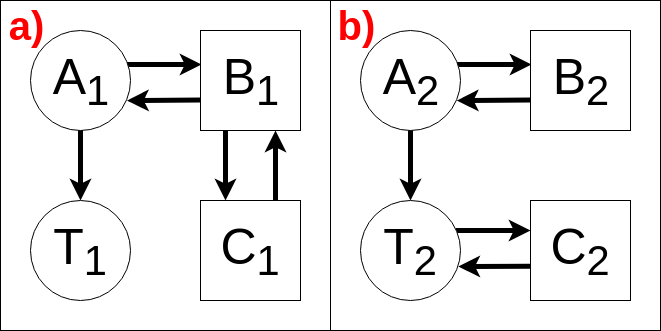
\includegraphics[scale=0.3]{Images/nestedCFA.png}
    \caption[Two CFAs with two loops each but structured differently.]{Two CFAs with two loops each but structured differently. Circles represent one location corresponding to a single instruction while squares represent subgraphs whose locations correspond to fall-through instructions.}
    \label{fig:pathExpNested}
\end{figure}
\\ \\
Figure \ref{fig:pathExpNested} illustrates a CFA which contains two nested loops and a CFA which contains two loops in serie. The circles represent locations of single instructions while squares represent subgraphs only containing locations of fall-through instructions. In Figure \ref{fig:pathExpNested}.a, the first loop is between $A_1$ and $B_1$ while the second loop is between $B_1$ and $C_1$. The $T_1$ node represents a top location. Let the length of the two nested loops, including the edges between the nodes in the illustration, be denoted as $L_{A_1B_1}$ and $L_{B_1C_1}$ respectively. Furthermore, assume that there is a maximum allowed length of the paths denoted by $L_{lim}$.
\\ \\ 
If one would not use any loops, there is only one path along the edge from $A_1$ to $T_1$. Otherwise, if one would only use the loop between $A_1$ and $B_1$, the number of possible paths is approximately $L_{lim}/L_{A_1B_1}$ since each iteration of the loop results in a new path. Furthermore, if both loops are allowed, for each number of iterations in the AB loop $I_{A_1B_1}$, there are $(L_{lim}-I_{A_1B_1}*L_{A_1B_1}-1)/L_{B_1C_1}$ iterations in the $B_1C_1$ loop.
%Since $(L_{lim}-I_{AB}*L_{AB}-1) < L_{lim}$, there are up to $(L_{lim}/L_{AB}*)(L_{lim}/L_{BC})$ possible paths using both loops.
\begin{figure}[!t]
    \centering
\begin{tcolorbox}
\begin{minted}[xleftmargin=5pt,linenos,fontsize=\footnotesize]{nasm}
SECTION .data
w1     db      'Too '
w2     db      'many '
w3     db      'paths', 0x0A
SECTION .text
global _start:

_start:
        push w1         ; push address of w1
        push 4          ; push length of w1
        call print      ; print 'Too '
        push w2         ; push address of w2
        push 5          ; push length of w2
        call print      ; print 'many '
        push w3         ; push address of w3
        push 6          ; push length of w3
        call print      ; print 'paths\n'
        jmp quit        ; Jump to quit
print:
        mov edx, [esp+4]; Length
        mov ecx, [esp+8]; Address of msg
        mov ebx, 1      ; Set ebx to standard out
        mov eax, 4      ; Set eax to the opcode of write
        int 0x80        ; Perform the syscall
        ret
quit:
        mov ebx, 0      ; Set ebx to 0
        mov eax, 1      ; Set eax to the opcode of exit
        int 0x80        ; Perform the syscall
\end{minted}
\end{tcolorbox}
\caption{An example of a small program with a large amount of possible paths.}
    \label{fig:pathExpProg}
\end{figure}
\\ \\
With the same reasoning, it can be seen that the the amount of paths scale similarly to loops in series. Consider the CFA in Figure \ref{fig:pathExpNested}.b. In this CFA, there are two loops in series. Similarly to the CFA with the nested loops, without using any loops, there is only one path between $A_2$ and $T_2$. Furthermore, if only the first loop is used, there are around $L_{lim}/L_{A_2B_2}$ possible paths since there is one possible path for each iteration of the loop. Moreover, if both paths are used and $I_{A_2B_2}$ denotes the number of iterations in the first loop, the number of possible iterations in the second loop is $(L_{lim}-I_{A_2B_2}*L_{A_2B_2}-1)/L_{B_2C_2}$. For CFA:s corresponding to larger programs the structure can be much more complicated and thus these CFA:s can have a much higher combination of loop iterations. Consequently, they are more likely to have a larger amount of paths.
\begin{figure}[!t]
    \centering
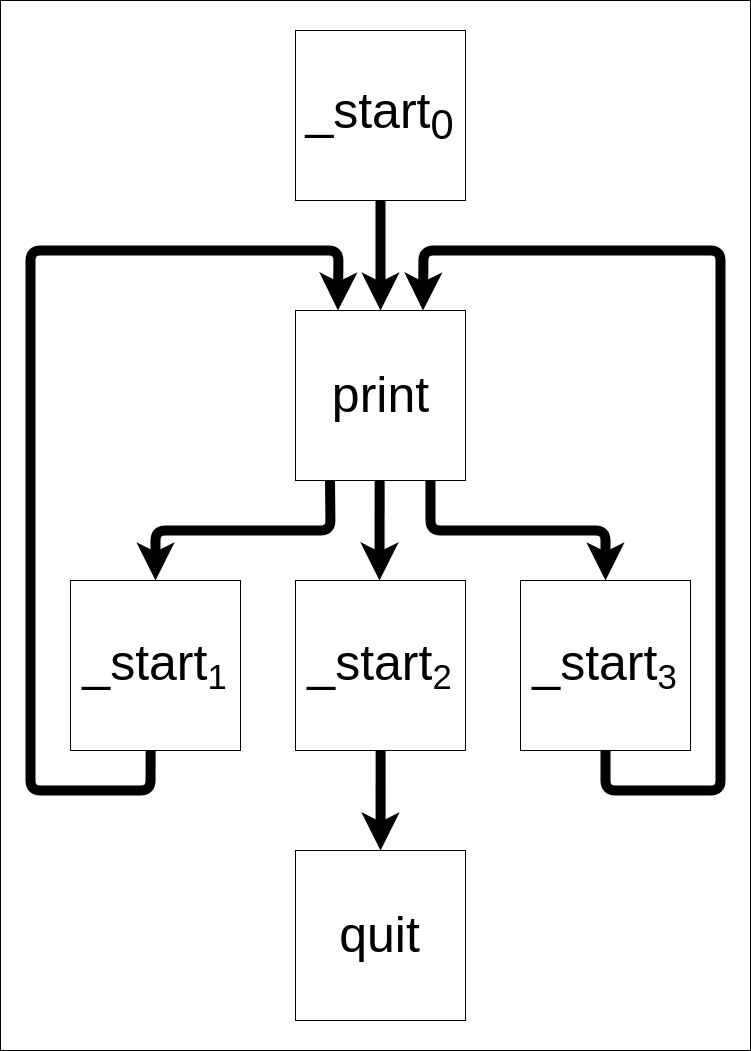
\includegraphics[scale=0.3]{Images/pathExpCFA.png}
    \caption{A simplified illustration of the CFA for the small program with a large amount of possible paths.}
    \label{fig:pathExpCFA}
\end{figure}
\\ \\
For example, consider the small synthetic program presented in Figure \ref{fig:pathExpProg}. This program contains a function $print$ which outputs a string to STDOUT. The $print$ function is called three times from three different locations. As such, the \it{ret} instruction at line 25 has three successors. These successors are line 12,15 and 18. However, since each node in the CFA only corresponds to a location, it is possible to identify paths which enter through a specific \it{call} instruction but exits through an edge from the location of the \it{ret} instruction which is not possible in practice if that specific \it{call} instruction was the last executed \it{call} instruction. For example, a path in the CFA could use the \it{call} instruction at line 14 to enter the $print$ function and then use the edge from line 25 to line 12 to arrive back at line 12. While this path is not possible in practice, it is possible in the CFA since states at the same locations are merged.
\\ \\
To illustrate how this creates a large number of paths, consider Figure \ref{fig:pathExpCFA} which is a simplification of the CFA for the program in Figure \ref{fig:pathExpProg}. This simplfied CFA represents locations for groups of fall through instructions by a square for ease of illustration. The $\_start_0$ corresponds to line 9 to 11, $\_start_1$ corresponds to line 12 to 14, $\_start_2$ corresponds to line 18 and $\_start_3$ corresponds to line 15 to 17. Furthermore, the $print$ and $quit$ represent line 20 to 25 and 27 to 29 respectively. Finally, assume thath the unresolved location is the location of the \it{ret} instruction for the $print$ function. 
\\ \\
As can be seen in the CFA, it is possible for a path to loop multiple times in either of the two loops. In fact, the paths may even constitute a mixture of the two loops in any particular order and with any number of iterations as long as the length of the path is lower than the limit on the amount of instructions. Executing a DFS limited to a depth of 100 instructions on this CFA, with the \it{ret} instruction marked as an unresolved location, yields 2047 unique paths. Furthermore, increasing the depth by 10 and 20 instructions increases the number of unique paths to 4095 and 8191 respectively. 
\\ \\
Moreover, by studying the graphs generated by angr for the GNU coreutils, it is possible to see that the number of instructions in these types of binaries are around a couple of thousands. As such, our earlier experiments would probably requrie a larger depth than 500 instructions for our approach to perform better than the state of the art. However, as can be observed in the example above, the number of uninque paths to an unresolved location can grow rapidly with the length limit of the path even for small examples. As such, our approach is not pragmatic unless it is possible to perform an efficient path extraction and storage.

%In general, for a CFA free from loops in series, we can thus see that the number of paths is bounded by $\Omega((L_{lim}/L_{max})^k)$ where $L_{max}$ is the length of the longest loop and $k$ is the number of nested loops\footnote{This can trivially be proved using an induction proof.}. 
%In essence, for loops in series without nested loops, the number of possible paths can be bounded by $\Omega((L_{lim}/L_{max})^k)$ where $L_{max}$ is the length of the longest loop and $k$ is the number of loops in series. %As we can not bound k, the amount of paths shorter than $L_{lim}$ could be large.



\chapter{Discussion and Future Work}\label{chap:discussionAndConclusions}
\fbcomment{\color{red}Goal: Discuss the results and draw conclusions}
%The main findings are highlighted and critically evaluated against the background of the study's assumptions and limitations.
%The project results are interpreted or discussed in a broader context; opinions and personal comments are well founded and supported by the results.
%The conclusions are reasonable, concrete and correspond to the question.
%Concerning CFGEmulated
In this section we provide a brief discussion where we summarize what has been performed in the thesis as well as what conclusions could be drawn. Additionally, we discuss how our approach can be modified for other under-approximation techniques. Thereafter, we describe possible future work to our contribution. Among other things, we suggest using white-box fuzzing as an under-approximation and evaluating other abstract domains than the constant propagation and strided interval domain.
\section{Discussion}
In this thesis, we addressed the problem of control flow reconstruction in the presence of indirect jumps. Initially, the differences between various types of instructions were explained. Furthermore, we described the difference between a BBG and a CFA as well as why a CFA can be extended to be more expressive than a BBG. Hence, motivating our design choice of reconstructing a CFA rather than a BBG. Additionally, the various static and dynamic analysis techniques were described and we motivated why DSE could be an interesting under-approximation candidate. Moreover, we introduced dataflow analysis.
\\ \\
Furthermore, the Jakstab tool that was applied to over-approximate the control flow using abstract interpretation, was introduced. Then, the advantages and disadvantages of adopting strided intervals as the abstract domain rather than constant propagation, were discussed. Thereafter, the CPA, CPA+ and Jakstab algorithms were explained and we introduced our own modifications to the Jakstab algorithm to enable the inclusion of additional control flow edges stemming from DSE.
\\ \\ 
The modifications we performed to the Jakstab algorithm enabled the usage of under-approximation with DSE to improve the soundness of the reconstructed control flow automaton. In fact, the two version of the ACFR algorithms that we introduced in section \ref{sec:modsToCPA} abstract from the under-approximation in a modular form. As such, one could integrate another under-approximation technique into the alternating algorithms simply by modifying the semantics of the DSE function at line 31 and line 33 in the pseudo codes presented in Figure \ref{fig:ACFR1} and \ref{fig:ACFR2} respectively.
\\ \\
After explaining the required modifications to the Jakstab algorithm, we provided and explained pseudo codes for ensuring that the symbolic execution would follow a set of provided paths and extract the successors of a set of target program locations. Then, we presented a small set of handcrafted examples that were used to illustrate the differences between the two versions of our algorithm as well as the advantages of using DSE for under-approximation of control flow. Thereafter, our abstract interpretation and DSE based alternating approach was implemented and evaluated using a set of metrics derived from earlier work in the field.
\\ \\
Throughout the thesis, we presented a set of synthetic binaries. These binaries were used for an initial evaluation of the tool. The results of the experiments with the synthetic binaries suggested that our algorithm can be advantageous for multiple challenging binaries. Furthermore, we then proceeded to evaluate our alternating approach on the five smallest binaries of the GNU coreutils. 
\\ \\
The results of the GNU coreutils evaluations showed no difference between the two version of our algorithm. Moreover, they suggested that the strided interval analysis suffered in performance when encountering particularly challening loops and that the requirement of extracting all possible paths from the program entry to a set of targets was not feasible in practice. Additionally, for constant propagation, it showed that the soundness could be increased by applying constant propagation with DSE rather than pure constant propagation. Finally, we explained the challenging type of loops that could thwart the strided interval based analyses and described why we believe a large amount of possible paths to be the reason for the high memory requirements of our algorithm.
\\ \\
From our results, a first conclusion was that our modifications to the widening operator resulted in strided interval analyses which could not reach a fixpoint within a reasonable amount of time when the subject program contained loops with a different amount of \it{call} and \it{ret} instructions. This suggested that strided intervals are not suitable for over-apprxoimations of CFAs unless they use an overly conservative widening operator. A second conclusion we drew was that alternating approaches which are dependent on extractions of paths are very limited since the amount of possible paths in the CFA can be very large.

%Snapshot directed symbolic execution and resume instead of restarting
%Backward reachability algorithm as described in FXE Paper?
%Relax one or more assumptions?
%Widening operator of interval domain, over-approximate when a certain location has been widened more than x times.
%In our work, the amount of successors asked for each instruction was set to 5. 
%Heuristic for the number of smt solves?
\section{Future Work}
\fbcomment{\color{red}Goal: Describe how the work in this thesis can be extended.}
As the strided interval based analyses struggled with loops with a different amount of \it{call} and \it{ret} instructions, it could be interesting to detect and exclude those. This would, however, require the execution of an algorithm for detection of cycles in a graph such as Tarjan's or Kosaraju's algorithm. Once a cycle is found, it could trivially be determined if it should be excluded by counting its \it{call} and \it{ret} instructions. This would, however, add the assumption that the binary does not contain any loops with a different amount of \it{call} and \it{ret} instructions since they have to be assumed to be a product of the over-approximation. This could possibly exclude malware and other types of malicious binaries as target binaries.
\\ \\
Another approach could be to identify these loops and force the widening operator to over-approximate the possible \it{esp} values to $\top$. This would enable the analysis to continue without getting stuck infinitely. However, this would require some heuristic to determine at which instruction the widening operator should be over-approximated to $\top$. For example, a loop might contain a different number of \it{call} and \it{ret} instruction but there might exists a path that uses only a small portion of the loop and continues the execution with some other instructions. 
\\ \\
Thus, at the execution of each instruction, it would be required to know if one is revisiting an instruction in a problematic loop. However, to determine if this is the case, it would be required to know previously executed instructions leading to the current one. As this does not scale well in terms of memory usage, some heuristic would be required that can determine if the instruction in a problematic loop is revisited with less saved information than all previously executed instructions.
\\ \\
An additional problem that was encountered was the large memory requirement as a result of unrolling the loops in the CFA into a large amount of length limited paths. To limit this memory usage, one alternative could be to determine how many iterations are possible for each loop and only extract the paths with that particular number of iterations. This could possibly be conducted by identifying loop variants and bounding these. However, this is an undecidable problem in general since its solution would mean a solution to the halting problem. As such, loops which can not be determined to have a fixed number of possible iterations would require unrolling. Nevertheless, it could be interesting to investigate to what extent this method could decrease the memory requirements of our approach as it could still decrease memory usage even if it couldn't determine the number of possible iterations for all loops.
\\ \\
Another alliterative could be to find a more efficient storage method than to simply store all paths shorter than a fixed length as done in this thesis. For example, it could be interesting to utilize a cycle detection algorithm to detect the cycles to avoid multiple entries for paths which only different in the number of loop iterations performed. Thus, the loop would only have to be stored once together with some meta data marking the sequence of instructions as a loop. This would require further modifications to the pseudo codes presented in section \ref{sec:DSEPseudo} but would decrease the storage requirements of the paths, maybe resulting in a more scalable algorithm.
\\ \\
In addition to studying how to avoid the storage of a large amount of paths, it could alse be interesting to study different abstract domains for the over-approximation. When the ACFR algorithms were developed, it was ensured that they wouldn't disable the usage of abstract domains which requrie precision elements and precision refinement. As such, it could be interesting to evaluate our alternating approach using some of the other abstract domains that were originally developed for Jakstab. Furthermore, Jakstab also includes the possibility to combine multiple abstract domains into a combined abstract domain. As such, it might also be of interest to study which groups of abstract domains perform best  with DSE.
\\ \\
Furthermore, it could also be of value to study other under-approximation approaches than DSE in the context of our alternating algorithms. As briefly discussed in the previous section, this should not be more complicated than to modify the semantics of the DSE function. For example, the DSE funciton could instead utilize the provided paths and targets for performing white box fuzz testing\cite{automatedFuzzing} to acquire successor locations of the target locations. It could then be interesting to evaluate if the white-box fuzzing can determine more successors than DSE.

% Print the bibliography (and make it appear in the table of contents)
\begin{otherlanguage}{australian}%Australian ensure that the date format is European rather than American..
\printbibliography[heading=bibintoc]
\end{otherlanguage}

\appendix
\chapter{Extensive Results}

\begin{table}[ht]
\centering
\scalebox{0.5}{
\begin{tabular}{?l|l|l?l|l|l?l|l?l|l|l?l|l|l|l|l?}
\Xhline{2\arrayrulewidth}
\textbf{Binary} & \textbf{Mode} & \textbf{Instructions} & \textbf{$\mathcal{A}_{E_I,E_G}$} & \textbf{$\mathcal{P}_{E_I,E_G}$} & \textbf{$\mathcal{S}_{E_I,E_G}$} & \textbf{uTops} & \textbf{Tops} & \textbf{$\mathcal{A}_{E_I,E_{TF}}$} & \textbf{$\mathcal{P}_{E_I,E_{TF}}$} & \textbf{$\mathcal{S}_{E_I,E_{TF}}$} & \textbf{$T_{CPA}$} & \textbf{$T_{DFS}$} & \textbf{$T_{DSE}$} & \textbf{$T_{Other}$}\\ \Xhline{2\arrayrulewidth} 
badCall & c & 4 & 14.81\% & 40.74\% & 66.67\% & 1 & 1 & 100.0\% & 75.0\% & 50.0\% & 301ms & 0ms & 0ms & 110ms\\ \hline
badCall & cD & 7 & 20.0\% & 60.0\% & 100.0\% & 0 & 1 & 83.33\% & 83.33\% & 83.33\% & 269ms & 0ms & 1202ms & 203ms\\ \hline
badCall & i & 7 & 85.71\% & 92.86\% & 100.0\% & 0 & 0 & 85.71\% & 92.86\% & 100.0\% & 254ms & 0ms & 0ms & 139ms\\ \hline
badCall & iD & 7 & 85.71\% & 92.86\% & 100.0\% & 0 & 0 & 85.71\% & 92.86\% & 100.0\% & 247ms & 0ms & 0ms & 207ms\\ \Xhline{2\arrayrulewidth} 
badIndMemJmp & c & 1 & 22.22\% & 44.44\% & 66.67\% & 1 & 1 & - & - & 0.0\% & 240ms & 0ms & 0ms & 123ms\\ \hline
badIndMemJmp & cD & 1 & 22.22\% & 44.44\% & 66.67\% & 0 & 1 & - & - & 0.0\% & 170ms & 3ms & 1684ms & 220ms\\ \hline
badIndMemJmp & i & 1 & 0.0\% & 0.0\% & 0.0\% & 0 & 0 & 0.0\% & 0.0\% & 0.0\% & 95ms & 0ms & 0ms & 159ms\\ \hline
badIndMemJmp & iD & 1 & 0.0\% & 0.0\% & 0.0\% & 0 & 0 & 0.0\% & 0.0\% & 0.0\% & 96ms & 0ms & 0ms & 217ms\\ \Xhline{2\arrayrulewidth} 
branch & c & 17 & 20.45\% & 60.23\% & 100.0\% & 1 & 1 & 94.12\% & 91.5\% & 88.89\% & 320ms & 0ms & 0ms & 123ms\\ \hline
branch & cD & 17 & 20.45\% & 60.23\% & 100.0\% & 0 & 1 & 94.12\% & 91.5\% & 88.89\% & 442ms & 2ms & 2019ms & 177ms\\ \hline
branch & i & 17 & 94.74\% & 97.37\% & 100.0\% & 0 & 0 & 94.74\% & 97.37\% & 100.0\% & 477ms & 0ms & 0ms & 121ms\\ \hline
branch & iD & 17 & 94.74\% & 97.37\% & 100.0\% & 0 & 0 & 94.74\% & 97.37\% & 100.0\% & 473ms & 0ms & 0ms & 208ms\\ \Xhline{2\arrayrulewidth} 
callRet & c & 2 & 8.33\% & 24.17\% & 40.0\% & 1 & 1 & 100.0\% & 60.0\% & 20.0\% & 280ms & 0ms & 0ms & 134ms\\ \hline
callRet & cD & 6 & 17.86\% & 58.93\% & 100.0\% & 0 & 1 & 80.0\% & 80.0\% & 80.0\% & 274ms & 1ms & 1152ms & 183ms\\ \hline
callRet & i & 6 & 83.33\% & 91.67\% & 100.0\% & 0 & 0 & 83.33\% & 91.67\% & 100.0\% & 248ms & 0ms & 0ms & 146ms\\ \hline
callRet & iD & 6 & 83.33\% & 91.67\% & 100.0\% & 0 & 0 & 83.33\% & 91.67\% & 100.0\% & 248ms & 0ms & 0ms & 213ms\\ \Xhline{2\arrayrulewidth} 
cjmp & c & 11 & 90.91\% & 95.45\% & 100.0\% & 0 & 0 & 90.91\% & 95.45\% & 100.0\% & 290ms & 0ms & 0ms & 122ms\\ \hline
cjmp & cD & 11 & 90.91\% & 95.45\% & 100.0\% & 0 & 0 & 90.91\% & 95.45\% & 100.0\% & 282ms & 0ms & 0ms & 209ms\\ \hline
cjmp & i & 11 & 90.91\% & 95.45\% & 100.0\% & 0 & 0 & 90.91\% & 95.45\% & 100.0\% & 278ms & 0ms & 0ms & 150ms\\ \hline
cjmp & iD & 11 & 90.91\% & 95.45\% & 100.0\% & 0 & 0 & 90.91\% & 95.45\% & 100.0\% & 270ms & 0ms & 0ms & 226ms\\ \Xhline{2\arrayrulewidth} 
cjmpBitOp & c & 7 & 85.71\% & 92.86\% & 100.0\% & 0 & 0 & 85.71\% & 92.86\% & 100.0\% & 273ms & 0ms & 0ms & 129ms\\ \hline
cjmpBitOp & cD & 7 & 85.71\% & 92.86\% & 100.0\% & 0 & 0 & 85.71\% & 92.86\% & 100.0\% & 291ms & 0ms & 0ms & 183ms\\ \hline
cjmpBitOp & i & 8 & 75.0\% & 87.5\% & 100.0\% & 0 & 0 & 75.0\% & 87.5\% & 100.0\% & 260ms & 0ms & 0ms & 146ms\\ \hline
cjmpBitOp & iD & 8 & 75.0\% & 87.5\% & 100.0\% & 0 & 0 & 75.0\% & 87.5\% & 100.0\% & 247ms & 0ms & 0ms & 222ms\\ \Xhline{2\arrayrulewidth} 
conditionalTop & c & 11 & 33.33\% & 66.67\% & 100.0\% & 1 & 1 & 100.0\% & 78.95\% & 57.89\% & 312ms & 0ms & 0ms & 121ms\\ \hline
conditionalTop & cD & 11 & 33.33\% & 66.67\% & 100.0\% & 0 & 1 & 100.0\% & 78.95\% & 57.89\% & 285ms & 1ms & 1584ms & 209ms\\ \hline
conditionalTop & i & 11 & 33.33\% & 66.67\% & 100.0\% & 1 & 1 & 100.0\% & 78.95\% & 57.89\% & 319ms & 0ms & 0ms & 126ms\\ \hline
conditionalTop & iD & 11 & 33.33\% & 66.67\% & 100.0\% & 0 & 1 & 100.0\% & 78.95\% & 57.89\% & 270ms & 0ms & 2025ms & 234ms\\ \Xhline{2\arrayrulewidth} 
doubleCallRet & c & 17 & 9.47\% & 45.65\% & 81.82\% & 2 & 2 & 100.0\% & 86.36\% & 72.73\% & 318ms & 0ms & 0ms & 127ms\\ \hline
doubleCallRet & cD & 22 & 11.28\% & 55.64\% & 100.0\% & 0 & 2 & 95.24\% & 93.07\% & 90.91\% & 296ms & 0ms & 1593ms & 223ms\\ \hline
doubleCallRet & i & 22 & 95.65\% & 97.83\% & 100.0\% & 0 & 0 & 95.65\% & 97.83\% & 100.0\% & 304ms & 0ms & 0ms & 164ms\\ \hline
doubleCallRet & iD & 22 & 95.65\% & 97.83\% & 100.0\% & 0 & 0 & 95.65\% & 97.83\% & 100.0\% & 296ms & 0ms & 0ms & 225ms\\ \Xhline{2\arrayrulewidth} 
espAssignment & c & 9 & 16.33\% & 58.16\% & 100.0\% & 1 & 1 & 87.5\% & 87.5\% & 87.5\% & 311ms & 0ms & 0ms & 126ms\\ \hline
espAssignment & cD & 9 & 16.33\% & 58.16\% & 100.0\% & 1 & 1 & 87.5\% & 87.5\% & 87.5\% & 281ms & 5ms & 592ms & 328ms\\ \hline
espAssignment & i & 9 & 16.33\% & 58.16\% & 100.0\% & 1 & 1 & 87.5\% & 87.5\% & 87.5\% & 338ms & 0ms & 0ms & 138ms\\ \hline
espAssignment & iD & 9 & 16.33\% & 58.16\% & 100.0\% & 1 & 1 & 87.5\% & 87.5\% & 87.5\% & 282ms & 13ms & 578ms & 363ms\\ \Xhline{2\arrayrulewidth} 
indMemJmp & c & 6 & 83.33\% & 91.67\% & 100.0\% & 0 & 0 & 83.33\% & 91.67\% & 100.0\% & 269ms & 0ms & 0ms & 122ms\\ \hline
indMemJmp & cD & 6 & 83.33\% & 91.67\% & 100.0\% & 0 & 0 & 83.33\% & 91.67\% & 100.0\% & 270ms & 0ms & 0ms & 202ms\\ \hline
indMemJmp & i & 6 & 83.33\% & 91.67\% & 100.0\% & 0 & 0 & 83.33\% & 91.67\% & 100.0\% & 246ms & 0ms & 0ms & 151ms\\ \hline
indMemJmp & iD & 6 & 83.33\% & 91.67\% & 100.0\% & 0 & 0 & 83.33\% & 91.67\% & 100.0\% & 247ms & 0ms & 0ms & 229ms\\ \Xhline{2\arrayrulewidth} 
infiniteLoop & c & 10 & 66.67\% & 83.33\% & 100.0\% & 0 & 0 & 66.67\% & 83.33\% & 100.0\% & 297ms & 0ms & 0ms & 132ms\\ \hline
infiniteLoop & cD & 10 & 66.67\% & 83.33\% & 100.0\% & 0 & 0 & 66.67\% & 83.33\% & 100.0\% & 299ms & 0ms & 0ms & 189ms\\ \hline
infiniteLoop$\triangle_{T}$ & i & 10 & 66.67\% & 83.33\% & 100.0\% & 0 & 0 & 66.67\% & 83.33\% & 100.0\% & 7141982ms & 0ms & 0ms & 63ms\\ \hline
infiniteLoop$\triangle_{T}$ & iD & 10 & 66.67\% & 83.33\% & 100.0\% & 0 & 0 & 66.67\% & 83.33\% & 100.0\% & 7141871ms & 0ms & 0ms & 114ms\\ \Xhline{2\arrayrulewidth} 
int & c & 9 & 88.89\% & 94.44\% & 100.0\% & 0 & 0 & 88.89\% & 94.44\% & 100.0\% & 268ms & 0ms & 0ms & 123ms\\ \hline
int & cD & 9 & 88.89\% & 94.44\% & 100.0\% & 0 & 0 & 88.89\% & 94.44\% & 100.0\% & 273ms & 0ms & 0ms & 197ms\\ \hline
int & i & 9 & 88.89\% & 94.44\% & 100.0\% & 0 & 0 & 88.89\% & 94.44\% & 100.0\% & 247ms & 0ms & 0ms & 148ms\\ \hline
int & iD & 9 & 88.89\% & 94.44\% & 100.0\% & 0 & 0 & 88.89\% & 94.44\% & 100.0\% & 239ms & 0ms & 0ms & 210ms\\ \Xhline{2\arrayrulewidth} 
kindConditionalTop & c & 8 & 26.83\% & 63.41\% & 100.0\% & 1 & 1 & 100.0\% & 81.82\% & 63.64\% & 300ms & 0ms & 0ms & 121ms\\ \hline
kindConditionalTop & cD & 8 & 26.83\% & 63.41\% & 100.0\% & 0 & 1 & 100.0\% & 81.82\% & 63.64\% & 274ms & 1ms & 1400ms & 194ms\\ \hline
kindConditionalTop & i & 8 & 26.83\% & 63.41\% & 100.0\% & 1 & 1 & 100.0\% & 81.82\% & 63.64\% & 291ms & 0ms & 0ms & 122ms\\ \hline
kindConditionalTop & iD & 8 & 26.83\% & 63.41\% & 100.0\% & 0 & 1 & 100.0\% & 81.82\% & 63.64\% & 261ms & 1ms & 1374ms & 205ms\\ \Xhline{2\arrayrulewidth}
\end{tabular}
}
\caption[Results of the synthetic benchmarks for the second version of the ACFR algorithm (Part 1).]{Results of the synthetic benchmarks for the second version of the ACFR algorithm (Part 1). Analyses which had to be interrupted as they did not finish within 2 hours are marked with $\triangle_{T}$.}
\label{tab:ACFR2Syn1}
\end{table}

\begin{table}[ht]
\centering
\scalebox{0.5}{
\begin{tabular}{?l|l|l?l|l|l?l|l?l|l|l?l|l|l|l|l?}
\Xhline{2\arrayrulewidth}
\textbf{Binary} & \textbf{Mode} & \textbf{Instructions} & \textbf{$\mathcal{A}_{E_I,E_G}$} & \textbf{$\mathcal{P}_{E_I,E_G}$} & \textbf{$\mathcal{S}_{E_I,E_G}$} & \textbf{uTops} & \textbf{Tops} & \textbf{$\mathcal{A}_{E_I,E_{TF}}$} & \textbf{$\mathcal{P}_{E_I,E_{TF}}$} & \textbf{$\mathcal{S}_{E_I,E_{TF}}$} & \textbf{$T_{CPA}$} & \textbf{$T_{DFS}$} & \textbf{$T_{DSE}$} & \textbf{$T_{Other}$}\\ \Xhline{2\arrayrulewidth} 
longRegisterEquals & c & 14 & 15.38\% & 57.69\% & 100.0\% & 1 & 1 & 66.67\% & 83.33\% & 100.0\% & 303ms & 0ms & 0ms & 133ms\\ \hline
longRegisterEquals & cD & 14 & 15.38\% & 57.69\% & 100.0\% & 1 & 1 & 66.67\% & 83.33\% & 100.0\% & 301ms & 1ms & 949ms & 193ms\\ \hline
longRegisterEquals & i & 14 & 15.38\% & 57.69\% & 100.0\% & 1 & 1 & 66.67\% & 83.33\% & 100.0\% & 308ms & 0ms & 0ms & 126ms\\ \hline
longRegisterEquals & iD & 14 & 15.38\% & 57.69\% & 100.0\% & 1 & 1 & 66.67\% & 83.33\% & 100.0\% & 258ms & 2ms & 605ms & 246ms\\ \Xhline{2\arrayrulewidth} 
memCallRet & c & 4 & 10.53\% & 33.83\% & 57.14\% & 1 & 1 & 100.0\% & 71.43\% & 42.86\% & 284ms & 0ms & 0ms & 124ms\\ \hline
memCallRet & cD & 8 & 16.67\% & 58.33\% & 100.0\% & 0 & 1 & 85.71\% & 85.71\% & 85.71\% & 271ms & 0ms & 1092ms & 182ms\\ \hline
memCallRet & i & 8 & 87.5\% & 93.75\% & 100.0\% & 0 & 0 & 87.5\% & 93.75\% & 100.0\% & 255ms & 0ms & 0ms & 161ms\\ \hline
memCallRet & iD & 8 & 87.5\% & 93.75\% & 100.0\% & 0 & 0 & 87.5\% & 93.75\% & 100.0\% & 245ms & 0ms & 0ms & 218ms\\ \Xhline{2\arrayrulewidth} 
minimalistic & c & 5 & 10.71\% & 20.36\% & 30.0\% & 1 & 1 & 100.0\% & 60.0\% & 20.0\% & 268ms & 0ms & 0ms & 146ms\\ \hline
minimalistic & cD & 35 & 10.53\% & 55.26\% & 100.0\% & 0 & 3 & 47.06\% & 63.53\% & 80.0\% & 574ms & 44ms & 4615ms & 725ms\\ \hline
minimalistic & i & 11 & 19.35\% & 39.68\% & 60.0\% & 1 & 1 & 100.0\% & 75.0\% & 50.0\% & 365ms & 0ms & 0ms & 130ms\\ \hline
minimalistic$\triangle_{T}$ & iD & 15 & 13.68\% & 46.84\% & 80.0\% & 1 & 2 & 100.0\% & 82.5\% & 65.0\% & 7148204ms & 7ms & 686ms & 293ms\\ \Xhline{2\arrayrulewidth} 
nestedCallRet & c & 3 & 9.68\% & 26.27\% & 42.86\% & 1 & 1 & 100.0\% & 64.29\% & 28.57\% & 271ms & 0ms & 0ms & 133ms\\ \hline
nestedCallRet & cD & 8 & 10.94\% & 55.47\% & 100.0\% & 0 & 2 & 83.33\% & 77.38\% & 71.43\% & 279ms & 1ms & 1760ms & 199ms\\ \hline
nestedCallRet & i & 8 & 87.5\% & 93.75\% & 100.0\% & 0 & 0 & 87.5\% & 93.75\% & 100.0\% & 253ms & 0ms & 0ms & 154ms\\ \hline
nestedCallRet & iD & 8 & 87.5\% & 93.75\% & 100.0\% & 0 & 0 & 87.5\% & 93.75\% & 100.0\% & 278ms & 0ms & 0ms & 211ms\\ \Xhline{2\arrayrulewidth} 
registerEquals & c & 8 & 15.15\% & 57.58\% & 100.0\% & 1 & 1 & 62.5\% & 81.25\% & 100.0\% & 291ms & 0ms & 0ms & 133ms\\ \hline
registerEquals & cD & 8 & 15.15\% & 57.58\% & 100.0\% & 1 & 1 & 62.5\% & 81.25\% & 100.0\% & 268ms & 1ms & 624ms & 206ms\\ \hline
registerEquals & i & 8 & 15.15\% & 57.58\% & 100.0\% & 1 & 1 & 62.5\% & 81.25\% & 100.0\% & 299ms & 0ms & 0ms & 116ms\\ \hline
registerEquals & iD & 8 & 15.15\% & 57.58\% & 100.0\% & 1 & 1 & 62.5\% & 81.25\% & 100.0\% & 263ms & 1ms & 640ms & 216ms\\ \Xhline{2\arrayrulewidth} 
sequentialCallRet & c & 2 & 10.34\% & 26.6\% & 42.86\% & 1 & 1 & 100.0\% & 57.14\% & 14.29\% & 269ms & 0ms & 0ms & 121ms\\ \hline
sequentialCallRet & cD & 7 & 20.59\% & 60.29\% & 100.0\% & 0 & 1 & 83.33\% & 77.38\% & 71.43\% & 277ms & 22ms & 3644ms & 655ms\\ \hline
sequentialCallRet & i & 7 & 87.5\% & 93.75\% & 100.0\% & 0 & 0 & 87.5\% & 93.75\% & 100.0\% & 271ms & 0ms & 0ms & 150ms\\ \hline
sequentialCallRet & iD & 7 & 87.5\% & 93.75\% & 100.0\% & 0 & 0 & 87.5\% & 93.75\% & 100.0\% & 264ms & 0ms & 0ms & 222ms\\ \Xhline{2\arrayrulewidth} 
stackBO & c & 13 & 37.23\% & 59.31\% & 81.4\% & 1 & 1 & 100.0\% & 63.95\% & 27.91\% & 309ms & 0ms & 0ms & 132ms\\ \hline
stackBO & cD & 13 & 37.23\% & 59.31\% & 81.4\% & 0 & 1 & 100.0\% & 63.95\% & 27.91\% & 281ms & 0ms & 1620ms & 221ms\\ \hline
stackBO & i & 22 & 95.45\% & 72.15\% & 48.84\% & 0 & 0 & 95.45\% & 72.15\% & 48.84\% & 278ms & 0ms & 0ms & 154ms\\ \hline
stackBO & iD & 22 & 95.45\% & 72.15\% & 48.84\% & 0 & 0 & 95.45\% & 72.15\% & 48.84\% & 264ms & 0ms & 0ms & 218ms\\ \Xhline{2\arrayrulewidth} 
trueTop & c & 7 & 34.29\% & 67.14\% & 100.0\% & 1 & 1 & 100.0\% & 75.0\% & 50.0\% & 283ms & 0ms & 0ms & 131ms\\ \hline
trueTop & cD & 7 & 34.29\% & 67.14\% & 100.0\% & 0 & 1 & 100.0\% & 75.0\% & 50.0\% & 265ms & 0ms & 1847ms & 202ms\\ \hline
trueTop & i & 7 & 34.29\% & 67.14\% & 100.0\% & 1 & 1 & 100.0\% & 75.0\% & 50.0\% & 275ms & 0ms & 0ms & 109ms\\ \hline
trueTop & iD & 7 & 34.29\% & 67.14\% & 100.0\% & 0 & 1 & 100.0\% & 75.0\% & 50.0\% & 256ms & 0ms & 2121ms & 209ms\\ \Xhline{2\arrayrulewidth} 
twoVars & c & 7 & 18.37\% & 46.68\% & 75.0\% & 1 & 1 & 100.0\% & 79.17\% & 58.33\% & 293ms & 0ms & 0ms & 143ms\\ \hline
twoVars & cD & 11 & 22.64\% & 61.32\% & 100.0\% & 0 & 1 & 90.91\% & 87.12\% & 83.33\% & 283ms & 2ms & 1292ms & 201ms\\ \hline
twoVars & i & 7 & 18.37\% & 46.68\% & 75.0\% & 1 & 1 & 100.0\% & 79.17\% & 58.33\% & 298ms & 0ms & 0ms & 145ms\\ \hline
twoVars & iD & 11 & 22.64\% & 61.32\% & 100.0\% & 0 & 1 & 90.91\% & 87.12\% & 83.33\% & 249ms & 1ms & 1388ms & 249ms\\ \Xhline{2\arrayrulewidth} 
xyz & c & 10 & 16.95\% & 50.14\% & 83.33\% & 1 & 1 & 100.0\% & 87.5\% & 75.0\% & 317ms & 0ms & 0ms & 118ms\\ \hline
xyz & cD & 13 & 19.35\% & 59.68\% & 100.0\% & 0 & 1 & 91.67\% & 91.67\% & 91.67\% & 280ms & 0ms & 1418ms & 212ms\\ \hline
xyz & i & 10 & 16.95\% & 50.14\% & 83.33\% & 1 & 1 & 100.0\% & 87.5\% & 75.0\% & 297ms & 0ms & 0ms & 139ms\\ \hline
xyz & iD & 13 & 19.35\% & 59.68\% & 100.0\% & 0 & 1 & 91.67\% & 91.67\% & 91.67\% & 262ms & 0ms & 1471ms & 242ms\\ \Xhline{2\arrayrulewidth}
\end{tabular}
}
\caption[Results of the synthetic benchmarks for the second version of the ACFR algorithm (Part 2).]{Results of the synthetic benchmarks for the second version of the ACFR algorithm (Part 2). Analyses which had to be interrupted as they did not finish within 2 hours are marked with $\triangle_{T}$.}
\label{tab:ACFR2Syn2}
\end{table}

%Corresponds to /results/gnuCoreutils/1Nov and /results/gnuCoreutils/7Nov/
\begin{table}[ht]
\centering
\scalebox{0.5}{
\begin{tabular}{?l|l|l?l|l|l?l|l?l|l|l?l|l|l|l|l?}
\Xhline{2\arrayrulewidth}
\textbf{Binary} & \textbf{Mode} & \textbf{Instructions} & \textbf{$\mathcal{A}_{E_I,E_G}$} & \textbf{$\mathcal{P}_{E_I,E_G}$} & \textbf{$\mathcal{S}_{E_I,E_G}$} & \textbf{uTops} & \textbf{Tops} & \textbf{$\mathcal{A}_{E_I,E_{TF}}$} & \textbf{$\mathcal{P}_{E_I,E_{TF}}$} & \textbf{$\mathcal{S}_{E_I,E_{TF}}$} & \textbf{$T_{CPA}$} & \textbf{$T_{DFS}$} & \textbf{$T_{DSE}$} & \textbf{$T_{Other}$}\\ \Xhline{2\arrayrulewidth} 
echo & c & 10 & 0.00211\% & 0.00757\% & 0.01302\% & 1 & 1 & 100.0\% & 50.00651\% & 0.01302\% & 288ms & 0ms & 0ms & 310ms\\ \hline
echo $\triangle_{M}$ & cD & 59 & 0.00328\% & 0.04216\% & 0.08103\% & 0 & 4 & 100.0\% & 50.04052\% & 0.08103\% & 1147ms & 47ms & 3983ms & 687ms\\ \hline
echo $\triangle_{T}$ & i & 1253 & 0.03355\% & 0.94863\% & 1.86372\% & 9 & 9 & 91.47727\% & 46.6705\% & 1.86372\% & 7155590ms & 0ms & 0ms & 218ms\\ \hline
echo $\triangle_{T}$ & iD & 1346 & 0.03607\% & 1.02008\% & 2.00408\% & 9 & 9 & 92.02658\% & 47.01533\% & 2.00408\% & 7154816ms & 0ms & 0ms & 308ms\\ \Xhline{2\arrayrulewidth}
false & c & 10 & 0.00212\% & 0.00763\% & 0.01315\% & 1 & 1 & 100.0\% & 50.00657\% & 0.01315\% & 324ms & 0ms & 0ms & 304ms\\ \hline
false $\triangle_{M}$ & cD & 59 & 0.00329\% & 0.04255\% & 0.0818\% & 0 & 4 & 100.0\% & 50.0409\% & 0.0818\% & 1531ms & 39ms & 4840ms & 975ms\\ \hline
false $\triangle_{T}$ & i & 1253 & 0.03365\% & 0.95756\% & 1.88147\% & 9 & 9 & 91.47727\% & 46.67937\% & 1.88147\% & 7154597ms & 0ms & 0ms & 221ms\\ \hline
false $\triangle_{T}$ & iD & 1346 & 0.03619\% & 1.02968\% & 2.02317\% & 9 & 9 & 92.02658\% & 47.02487\% & 2.02317\% & 7153839ms & 0ms & 0ms & 285ms\\ \Xhline{2\arrayrulewidth}
make-prime-list & c & 10 & 0.00221\% & 0.00814\% & 0.01407\% & 1 & 1 & 100.0\% & 50.00703\% & 0.01407\% & 291ms & 0ms & 0ms & 277ms\\ \hline
make-prime-list $\triangle_{M}$ & cD & 59 & 0.00343\% & 0.04549\% & 0.08755\% & 0 & 4 & 100.0\% & 50.04377\% & 0.08755\% & 1111ms & 34ms & 3503ms & 666ms\\ \hline
make-prime-list $\triangle_{T}$ & i & 1346 & 0.03771\% & 1.10144\% & 2.16518\% & 9 & 9 & 92.02658\% & 47.09588\% & 2.16518\% & 7154939ms & 0ms & 0ms & 210ms\\ \hline
make-prime-list $\triangle_{T}$ & iD & 1346 & 0.03771\% & 1.10144\% & 2.16518\% & 9 & 9 & 92.02658\% & 47.09588\% & 2.16518\% & 7153194ms & 0ms & 0ms & 270ms\\ \Xhline{2\arrayrulewidth}
printenv & c & 10 & 0.0021\% & 0.00745\% & 0.0128\% & 1 & 1 & 100.0\% & 50.0064\% & 0.0128\% & 287ms & 0ms & 0ms & 312ms\\ \hline
printenv $\triangle_{M}$ & cD & 59 & 0.00326\% & 0.04147\% & 0.07967\% & 0 & 4 & 100.0\% & 50.03984\% & 0.07967\% & 1196ms & 34ms & 4041ms & 755ms\\ \hline
printenv $\triangle_{T}$ & i & 1253 & 0.03332\% & 0.93292\% & 1.83251\% & 9 & 9 & 91.47727\% & 46.65489\% & 1.83251\% & 7153311ms & 0ms & 0ms & 211ms\\ \hline
printenv $\triangle_{T}$ & iD & 1346 & 0.03583\% & 1.00317\% & 1.97052\% & 9 & 9 & 92.02658\% & 46.99855\% & 1.97052\% & 7154729ms & 0ms & 0ms & 354ms\\ \Xhline{2\arrayrulewidth}
true & c & 10 & 0.00212\% & 0.00763\% & 0.01315\% & 1 & 1 & 100.0\% & 50.00657\% & 0.01315\% & 303ms & 0ms & 0ms & 305ms\\ \hline
true $\triangle_{M}$ & cD & 59 & 0.00329\% & 0.04255\% & 0.0818\% & 0 & 4 & 100.0\% & 50.0409\% & 0.0818\% & 1185ms & 29ms & 3795ms & 715ms\\ \hline
true $\triangle_{T}$ & i & 1253 & 0.03365\% & 0.95756\% & 1.88147\% & 9 & 9 & 91.47727\% & 46.67937\% & 1.88147\% & 7153809ms & 0ms & 0ms & 219ms\\ \hline
true $\triangle_{T}$ & iD & 1346 & 0.03619\% & 1.02968\% & 2.02317\% & 9 & 9 & 92.02658\% & 47.02487\% & 2.02317\% & 7156424ms & 0ms & 0ms & 289ms\\ \Xhline{2\arrayrulewidth}
\end{tabular}
}
\caption[Evaluation of the 5 smallest GNU coreutils binaries using the second version of the ACFR algorithm.]{Evaluation of the 5 smallest GNU coreutils binaries using the second version of the ACFR algorithm. Analyses which had to be interrupted after 2 hours and analyses that terminated because of insufficient memory are marked with $\triangle_{T}$ and $\triangle_{M}$ respectively.}
\label{tab:ACFR2GNUCoreutils}
\end{table}

\begin{table}[ht]
\centering
\scalebox{0.5}{
\begin{tabular}{|l|l|l|l|l|l|l|l|l|l|l|}
\Xhline{2\arrayrulewidth}
\textbf{Binary} & \textbf{Mode} & \textbf{Instructions} & \textbf{States} & \textbf{DSE Requests} & \textbf{DSE Edges} & \textbf{$T_{CPA}$} & \textbf{$T_{DFS}$} & \textbf{$T_{DSE}$} & \textbf{$T_{Other}$}\\ \Xhline{2\arrayrulewidth} 
echo & cD & 59 & 161 & 4 & 4 & 1147ms & 47ms & 3983ms & 687ms\\ \hline
false & cD & 59 & 161 & 4 & 4 & 1531ms & 39ms & 4840ms & 975ms\\ \hline
make-prime-list & cD & 59 & 161 & 4 & 4 & 1111ms & 34ms & 3503ms & 666ms\\ \hline
printenv & cD & 59 & 161 & 4 & 4 & 1196ms & 34ms & 4041ms & 755ms\\ \hline
true & cD & 59 & 161 & 4 & 4 & 1185ms & 29ms & 3795ms & 715ms\\ \Xhline{2\arrayrulewidth}
\end{tabular}
}
\caption[]{}
\label{tab:unnamed}
\end{table}

%Corresponds to /results/gnuCoreutils/4NovDSEOnlyOnce and /results/gnuCoreutils/6NovDSEOnlyOnce


\begin{table}[ht]
\centering
\scalebox{0.5}{
\begin{tabular}{|l|l|l|l|l|l|l|}
\Xhline{2\arrayrulewidth}
\textbf{Binary} & \textbf{Mode} & \textbf{$T_{CPA}$} & \textbf{$T_{DFS}$} & \textbf{$T_{DSE}$} & \textbf{$T_{Other}$}\\ \Xhline{2\arrayrulewidth} 
echo & cD & 1147ms & 47ms & 3983ms & 687ms\\ \hline
false & cD & 1531ms & 39ms & 4840ms & 975ms\\ \hline
make-prime-list & cD & 1111ms & 34ms & 3503ms & 666ms\\ \hline
printenv & cD & 1196ms & 34ms & 4041ms & 755ms\\ \hline
true & cD & 1185ms & 29ms & 3795ms & 715ms\\ \Xhline{2\arrayrulewidth}
\end{tabular}
}
\caption[]{}
\label{tab:unnamed}
\end{table}


% Tailmatter inserts the back cover page (if enabled)
\tailmatter

\end{document}
